\documentclass[a4paper,makeidx,envcountchap,graybox,deutsch,ngerman,sectrefs]{svmono}
%\documentclass[envcountchap,graybox,deutsch,sectrefs]{svmono}
%%%%% eigene tempor�re Abk�rzungsliste, f�r die Zeit, bis einheitliche Schreibungen bestehen
\usepackage{tempshort}
%%  Von Springer empfohlene Pakete %% 
%%\documentclass[envcountsect,graybox,deutsch,sectrefs]{svmono}
\usepackage{chapterbib}
\usepackage{type1cm}
\usepackage[ansinew]{inputenc}
\usepackage{babel}
\usepackage[pdftex]{graphicx}  %PDF-Vektorgrafiken einbinden
\usepackage{newtxtext}         %Typischer Springer-Font
\usepackage{newtxmath}
\usepackage{multicol}
\usepackage{multirow}
\usepackage[bottom]{footmisc}  %Platziert alle Fu�noten unten  
\usepackage[nobreak]{cite}
%\usepackage{biblatex}
\usepackage{cancel}
\usepackage[absolute]{textpos}
\usepackage{pdflscape}
\usepackage{graphicx}
\usepackage{pdflscape}
\usepackage{ragged2e}
\usepackage[format=plain,
      justification=RaggedRight,
      singlelinecheck=false]
     {caption}
\usepackage{longtable}
%\usepackage{floatrow}
%\usepackage{mwe}
\usepackage[figuresright]{rotating}
\usepackage{bigints}
\let\laplace\relax  % Vermeidung der Fehlermeldung "\laplace already defined."
\usepackage{trfsigns}
%\usepackage{relsize}
\usepackage{tabulary}
%\usepackage{xcolor,colortbl}
%\usepackage[table]{xcolor}
\usepackage{blindtext}
%\usepackage{acronym}
%\usepackage{amsmath}
\usepackage{acro}
\usepackage{nomencl}


\usepackage{etoolbox}
%  Eigene Pakete %%
\usepackage{adjustbox}
\usepackage{wasysym}
\usepackage{gensymb}
\usepackage{float}
\usepackage{caption}
\usepackage[left=3cm, right=3cm, top=3cm, bottom=3cm, includeheadfoot]{geometry}

\usepackage{mathtools}   % Vermeidung der Fehlermeldung "Undefined control sequence \coloneqq."
% header and footer
\usepackage{fancyhdr}
\pagestyle{fancy}
\fancyhead{}
\fancyhead[LE,RO]\thepage
\renewcommand{\sectionmark}[1]{\markright{\thesection.\ #1}}
%\fancyhead[LO]{\nouppercase\leftmark}
%\fancyhead[RE]{\nouppercase\rightmark}
\fancyhead[LO]{\nouppercase\rightmark}
\fancyhead[RE]{\nouppercase\leftmark}
\fancyfoot{}
% svmono hat offenbar irgendwas merkw�rdig definiert, darum mu� hier verbreitert werden
%\addtolength\headwidth{25pt}
%\setlength{\headheight}{25pt}

%% Units
\usepackage{siunitx}
\sisetup{
  locale = US,
  per-mode = reciprocal, %symbol, % | reciprocal | fraction | ?
  exponent-product = \cdot,
  separate-uncertainty,
  %exponent-to-prefix,
  %prefixes-as-symbols = false,
  %list-units = brackets,% | single | repeat
  %range-units = brackets,% | single | repeat
  %multi-part-units = brackets,% | single | repeat
}
\usepackage{chngcntr}
\usepackage{booktabs}
\usepackage{slashed}
\usepackage{listings}
\usepackage{color} %red, green, blue, yellow, cyan, magenta, black, white
%\usepackage{color} %Einfache Farbendefinition -> von Graybox-Option ben�tigt
\usepackage{multirow}
\usepackage{longtable} %Tabellen �ber mehrere Seiten hinweg
\usepackage{framed} % von Graybox-Option ben�tigt
\usepackage[shortlabels]{enumitem} %Erweiterte Aufz�hloptionen
\usepackage{array}
\usepackage[xindy]{imakeidx} %Wortindex und Personenindex erstellen

\usepackage[hyphens]{url}
%\usepackage[breaklinks,colorlinks=true,linkcolor=black,urlcolor=blue,citecolor=black,filecolor=green,hyperfootnotes=false]{hyperref}
\usepackage[                                    %Hyperref erstellt ein Bookmark/Lesezeichen im PDF. siehe https://www.namsu.de/Extra/pakete/Hyperref.html
bookmarksopen=true,															%Das Lesezeichen ist ge�ffnet beim �ffnen der PDF.
bookmarksnumbered=true,                         %Zahlen werden im Bookmark angezeigt.   
plainpages=false,
pdfpagelabels,
colorlinks=true,                                %Links werden farbig dargestellt.
linkcolor=black, citecolor=black, urlcolor=cyan %Farben definieren.
]{hyperref}                                     %Sollte als letztes eingebunden werden, da es sehr viele Verweise und �nderungen erzeugt. Das Packet ist sehr stark, aber auch umfangreich ist. 
\pdfminorversion=5

\usepackage{hypcap}
\usepackage[record,section=section,stylemods={mcols},automake]{glossaries-extra}
\usepackage{glossary-longextra}
\setglossarystyle{long-name-sym-desc-loc}
\setabbreviationstyle[acronym]{long-short}

\definecolor{killA}{rgb}{.7,.3,.3}
\newcommand\killA[1]{\bgroup\color{killA}{\cancel{#1}}\egroup}
\newcommand\killB[1]{\bgroup\color{cyan!30!black}{\cancel{#1}}\egroup}
% typographisch korrekte Abk�rzungen (needs to be loaded after hyperref)
\usepackage{abbrev}
\newglossary*{bew}{Glossar}
\newglossary*{hm}{Glossar}
\newglossary*{adyn}{Glossar}
\newglossary*{kontmech}{Glossar}
\newglossary*{aero}{Glossar}
\newglossary*{edyn}{Glossar}
\newglossary*{srt}{Glossar}
\newglossary*{spo}{Glossar}
\newglossary*{optbas}{Glossar}
\newglossary*{optger}{Glossar}
\newglossary*{optatm}{Glossar}
\GlsXtrLoadResources[src={bew/gloss},type=bew]
\GlsXtrLoadResources[src={hm/gloss},type=hm]
\GlsXtrLoadResources[src={adyn/gloss},type=adyn]
\GlsXtrLoadResources[src={kontmech/gloss},type=kontmech]
\GlsXtrLoadResources[src={aero/gloss},type=aero]
\GlsXtrLoadResources[src={spo/gloss},type=spo]
\GlsXtrLoadResources[src={edyn/gloss},type=edyn]
\GlsXtrLoadResources[src={srt/gloss},type=srt]
\GlsXtrLoadResources[src={optbas/gloss},type=optbas]
\GlsXtrLoadResources[src={optger/gloss},type=optger]
\GlsXtrLoadResources[src={optatm/gloss},type=optatm]
\glssetcategoryattribute{bew}{indexname}{true}
%\renewcommand\index\newterm
%\newcolumntype{g}[1]{>{\RaggedRight\hspace{0pt}}p{#1}}
%\renewcommand\glslongextraNameAlign{g}
\renewcommand\glslongextraLocationAlign{@{\ ~\ }>{\raggedright}p{\glspagelistwidth}}
\definecolor{gls}{rgb}{.4,.4,.5}
\renewcommand*{\glstextformat}[1]{\textcolor{gls}{#1}}

%Absatzregeln
\clubpenalty = 30000 %Keine einzelnen Absatzzeilen
\widowpenalty = 30000
\setlength{\parindent}{0em} 
\newcolumntype{L}[1]{>{\raggedright\arraybackslash}p{#1}}
\newcolumntype{C}[1]{>{\centering\arraybackslash}p{#1}}
\newcolumntype{R}[1]{>{\raggedleft\arraybackslash}p{#1}}

\usepackage{xstring}

\newcommand\mfile[2]{%
\saveexpandmode\noexpandarg
\StrSubstitute{#2}{_}{\_}[\tmpname]
\restoreexpandmode
\href{MatlabDateien/\chapname/#1\tmpname}{\tmpname}}

%%% Hyperlinks zu MATLAB Dateien
%\newcommand\mlref[1]{\mfile{}{#1}}
%\newcommand\mlinclref[1]{\mfile{IncludeFolder/}{#1}}
%\newcommand\mldataref[1]{\mfile{Data/}{#1}}

%%% .. f�r ein Verzeichnis hoch
%%% . f�r aktuelle Verzeichnis
%% lokal: MatlabDateien/bew
%\newcommand\mlbewref[1]{\href{MatlabDateien/bew/#1}{#1}}
%% git: https://github.com/sn-code-inside/fingeruebungen-physik/tree/main/bew
\newcommand{\mlrefwithindex}[2]{%
  \index[mfiles]{#2}%   <-- Eintrag im M-File-Index mit aktueller Seitenzahl
  \href{https://github.com/sn-code-inside/fingeruebungen-physik/tree/main/#1/#2}{#2}%
}


%\newcommand\mlbewref[1]{\href{https://github.com/sn-code-inside/fingeruebungen-physik/tree/main/bew/#1}{#1}}
%\newcommand\mlbewdref[1]{\href{https://github.com/sn-code-inside/fingeruebungen-physik/tree/main/bew/Data/#1}{#1}}
%\newcommand\mlbewiref[1]{\href{https://github.com/sn-code-inside/fingeruebungen-physik/tree/main/bew/IncludeFolder/#1}{#1}}
%\newcommand\mlkontmechref[1]{\href{https://github.com/sn-code-inside/fingeruebungen-physik/tree/main/kontmech/#1}{#1}}
%\newcommand\mlkontmechdref[1]{\href{https://github.com/sn-code-inside/fingeruebungen-physik/tree/main/kontmech/Data/#1}{#1}}
%\newcommand\mlkontmechiref[1]{\href{https://github.com/sn-code-inside/fingeruebungen-physik/tree/main/kontmech/IncludeFolder/#1}{#1}}
%\newcommand\mlhmref[1]{\href{https://github.com/sn-code-inside/fingeruebungen-physik/tree/main/hm/#1}{#1}}
%\newcommand\mlhmdref[1]{\href{https://github.com/sn-code-inside/fingeruebungen-physik/tree/main/hm/Data/#1}{#1}}
%\newcommand\mlhmiref[1]{\href{https://github.com/sn-code-inside/fingeruebungen-physik/tree/main/hm/IncludeFolder/#1}{#1}}
%\newcommand\mladynref[1]{\href{https://github.com/sn-code-inside/fingeruebungen-physik/tree/main/adyn/#1}{#1}}
%\newcommand\mladyndref[1]{\href{https://github.com/sn-code-inside/fingeruebungen-physik/tree/main/adyn/Data/#1}{#1}}
%\newcommand\mladyniref[1]{\href{https://github.com/sn-code-inside/fingeruebungen-physik/tree/main/adyn/IncludeFolder/#1}{#1}}
%\newcommand\mledynref[1]{\href{https://github.com/sn-code-inside/fingeruebungen-physik/tree/main/edyn/#1}{#1}}
%\newcommand\mledyndref[1]{\href{https://github.com/sn-code-inside/fingeruebungen-physik/tree/main/edyn/Data/#1}{#1}}
%\newcommand\mledyniref[1]{\href{https://github.com/sn-code-inside/fingeruebungen-physik/tree/main/edyn/IncludeFolder/#1}{#1}}
%\newcommand\mloptbasref[1]{\href{https://github.com/sn-code-inside/fingeruebungen-physik/tree/main/optbas/#1}{#1}}
%\newcommand\mloptbasdref[1]{\href{https://github.com/sn-code-inside/fingeruebungen-physik/tree/main/optbas/Data/#1}{#1}}
%\newcommand\mloptbasiref[1]{\href{https://github.com/sn-code-inside/fingeruebungen-physik/tree/main/optbas/IncludeFolder/#1}{#1}}
%\newcommand\mloptspezref[1]{\href{https://github.com/sn-code-inside/fingeruebungen-physik/tree/main/optspez/#1}{#1}}
%\newcommand\mloptspezdref[1]{\href{https://github.com/sn-code-inside/fingeruebungen-physik/tree/main/optspez/Data/#1}{#1}}
%\newcommand\mloptspeziref[1]{\href{https://github.com/sn-code-inside/fingeruebungen-physik/tree/main/optspez/IncludeFolder/#1}{#1}}

\newcommand\mlbewref[1]{\mlrefwithindex{bew}{#1}}
\newcommand\mlbewdref[1]{\mlrefwithindex{bew/Data}{#1}}
\newcommand\mlbewiref[1]{\mlrefwithindex{bew/Include}{#1}}
\newcommand\mlkontmechref[1]{\mlrefwithindex{kontmech}{#1}}
\newcommand\mlkontmechdref[1]{\mlrefwithindex{kontmech/Data}{#1}}
\newcommand\mlkontmechiref[1]{\mlrefwithindex{kontmech/Include}{#1}}
\newcommand\mlhmref[1]{\mlrefwithindex{hm}{#1}}
\newcommand\mlhmdref[1]{\mlrefwithindex{hm/Data}{#1}}
\newcommand\mlhmiref[1]{\mlrefwithindex{hm/Include}{#1}}
\newcommand\mladynref[1]{\mlrefwithindex{adyn}{#1}}
\newcommand\mladyndref[1]{\mlrefwithindex{adyn/Data}{#1}}
\newcommand\mladyniref[1]{\mlrefwithindex{adyn/Include}{#1}}
\newcommand\mledynref[1]{\mlrefwithindex{edyn}{#1}}
\newcommand\mledyndref[1]{\mlrefwithindex{edyn/Data}{#1}}
\newcommand\mledyniref[1]{\mlrefwithindex{edyn/Include}{#1}}
\newcommand\mlsrtref[1]{\mlrefwithindex{edyn}{#1}}
\newcommand\mlsrtdref[1]{\mlrefwithindex{srt/Data}{#1}}
\newcommand\mlsrtiref[1]{\mlrefwithindex{srt/Include}{#1}}
\newcommand\mloptbasref[1]{\mlrefwithindex{optbas}{#1}}
\newcommand\mloptbasdref[1]{\mlrefwithindex{optbas/Data}{#1}}
\newcommand\mloptbasiref[1]{\mlrefwithindex{optbas/Include}{#1}}
\newcommand\mloptgerref[1]{\mlrefwithindex{optger}{#1}}
\newcommand\mloptgerdref[1]{\mlrefwithindex{optger/Data}{#1}}
\newcommand\mloptgeriref[1]{\mlrefwithindex{optger/Include}{#1}}
\newcommand\mloptatmref[1]{\mlrefwithindex{optatm}{#1}}
\newcommand\mloptatmdref[1]{\mlrefwithindex{optatm/Data}{#1}}
\newcommand\mloptatmiref[1]{\mlrefwithindex{optatm/Include}{#1}}


\newcommand\mlcmd[1]{\textcolor{cyan}{\texttt{#1}}}

%Grafikregeln
\graphicspath{{hm/graphs/}
							{bew/graphs/}
							{kontmech/graphs/}
							{hm/graphs/}
							{adyn/graphs/}
							{edyn/graphs/}
							{srt/graphs/}
							{kontmech/graphs/}
							{spo/graphs/}
							{aero/graphs/}
							{optbas/graphs/}
							{optger/graphs/}
							{optatm/graphs/}
							{solman/graphs/}}
\DeclareGraphicsExtensions{.pdf, .png, .jpg, .jpeg}
\def\figname{Abb}
\newcommand\figref[1]{\figname.\ \ref{abb:#1}}
\usepackage[labelfont=bf]{caption}

\usepackage{tocloft}
\usepackage{etoc}
\setlength\cftfignumwidth{30pt}

% Flatterrand links
\cftsetindents{chapter}{0em}{4em}
\cftsetindents{section}{1.5em}{4em}
\cftsetindents{subsection}{3.8em}{4em}

% flacher Rand links
%\cftsetindents{chapter}{0em}{4em}
%\cftsetindents{section}{0em}{4em}
%\cftsetindents{subsection}{0em}{4em}

\newcommand\partitle[1]{
\addcontentsline{toc}{part}{#1}
\begin{titlepage}
  %\vskip 60%\p@
  \begin{center}
    {\LARGE Finger�bungen der Physik -- #1 \par}
    \vskip 3em%
    {\large Michael Kaschke und Holger Cartarius\par}
  \end{center}
\end{titlepage}
}

%\newcommand\mlref[1]{\href{\chapname/matlab/#1}{#1}}
%\newcommand\mlinclref[1]{\href{\chapname/matlab/IncludeFolder/#1}{\color{cyan}{#1}}}

%Neue Kommandos
\def\eg{e.\,g.\  \ignorespaces}     %e.g. (im Englischen Dokument)
\newcommand{\lk}{\left(}        %gro�e runde Klammer (links)
\newcommand{\rk}{\right )}      %gro�e runde Klammer (rechts)
\newcommand{\lgk}{\left \{}     %gro�e geschweifte Klammer (links)
\newcommand{\rgk}{\right \}}    %gro�e geschweifte Klammer (rechts)
\newcommand{\lek}{\left [}      %gro�e eckige Klammer (links)
\newcommand{\rek}{\right ]}     %gro�e eckige Klammer (rechts)
\newcommand{\anf}[1]{\glqq#1\grqq}    %Deutsche Anf�hrungszeichen: \anf{}
\newcommand{\defined}{:=}				%Definition
\newcommand{\curl}{\text{\textbf{rot}}\,}	%Rotation-Operator curl()
\newcommand{\ket}[1]{|#1\rangle}		%Quantenmechanischer Zustand
\newcommand{\curvelintri}{\,\overset{\blacktriangle}{\smallfrown}}
\newcommand{\straighttri}{\blacktriangle}
\newcommand{\UT}{\text{UT}}
\newcommand{\UTC}{\text{UTC}}
\newcommand{\JD}{\text{JD}}
\newcommand{\JDE}{\text{JDE}}
\newcommand{\MJD}{\text{MJD}}
\newcommand{\TDT}{\text{TDT}}
\newcommand{\TT}{\text{TT}}
\newcommand{\NVS}{\text{Navier-Stokes-Gleichungen}}
\newcommand{\MWG}{\text{Max\-well-Gleich\-ungen}}
\newcommand{\HG}{\text{Helm\-holtz-Glei\-chung}}
\newcommand{\sHG}{\text{ska\-lare Helm\-holtz-Glei\-chung}}
\newcommand{\vHG}{\text{vek\-to\-riel\-le Helm\-holtz-Glei\-chung}}
\newcommand{\sHGn}{\text{ska\-laren Helm\-holtz-Glei\-chung}}
\newcommand{\vHGn}{\text{vek\-to\-riel\-len Helm\-holtz-Glei\-chung}}
\newcommand{\SRT}{\text{Spezielle Relativit�tstheorie}}
\newcommand{\sRT}{\text{speziellen Relativit�tstheorie}}
\newcommand{\EMW}{\text{Elek\-tro\-magne\-tische Wellen}}
\newcommand{\eMW}{\text{elek\-tro\-magne\-tische Wellen}}
\newcommand{\eme}{\text{elektromagnetische}}
\newcommand{\EMF}{\text{Elektromagnetisches Feld}}
\newcommand{\eMF}{\text{elektromagnetischen Feld}}
\newcommand{\RT}{\text{Relativit�tstheorie~}}
\newcommand{\au}{\mathrm{AE}}
\newcommand{\ET}{\text{ET}}
\newcommand{\TAI}{\text{TAI}}
\newcommand{\GMST}{\text{GMST}}
\newcommand{\LMST}{\text{LMST}}
\newcommand{\MESZ}{\text{MESZ}}
\newcommand{\KOS}{\text{Koordinatensystem }}
\newcommand{\DGL}{\text{Differentialgleichung }}
\newcommand{\NA}{\text{NA}}
\newcommand{\uA}{\text{u}}  %atomare Masseneinheit
\newcommand{\MOZ}{\text{MOZ}}
\newcommand{\grad}{\text{\textbf{grad}}\,}	%Gradient-Operator grad()
\newcommand{\uproman}[1]{\uppercase\expandafter{\romannumeral#1}}
\newcommand{\lowroman}[1]{\romannumeral#1\relax}
\newcommand\todo[1]{\textcolor{red}{TODO: #1}}
\renewcommand{\=}[1]{\stackrel{\text{#1}}{=}}  %Schrift �ber Gleich-Zeichen
\renewcommand{\d}{\partial}
\newcommand{\abs}[1]{\left\vert#1\right\vert}            %Betragsklammern
\renewcommand{\Re}{\mathrm{Re}}                          %Realteil
\renewcommand{\Im}{\mathrm{Im}}                          %Imagin�rteil
\renewcommand{\im}{\mathrm{i}}                           %Imagin�re Einheite
\newcommand{\epsi}{\varepsilon} 
\renewcommand{\exp}{\mathrm{exp}}                        %Exponentialfunktion
\newcommand{\keff}{k_\text{eff}}
\newcommand{\con}{\text{const}}
\newcommand{\conv}{\vec{const}}
\newcommand{\nL}{n_\text{L}}    %n_L Brechungsindex Linse
\newcommand{\PL}{\mathcal{P}_}  %Legendre Polynome
\newcommand{\Pl}{\mathcal{P}}   %Legendre Polynome �ltere Variante 
\newcommand{\RB}{\mathcal{R}}   %Allgemeine Radial_Bessel_Funktion
\newcommand{\ve}{\vec{e}}   %Einheitsvektor
\newcommand{\vr}{\vec{r}}   %Ortsvektor
\newcommand{\vk}{\vec{k}}   %Wellenzahlvektor
\newcommand{\vp}{\vec{p}}   %Impulsvektor
\newcommand\PLZ[2]{\mathcal{P}_{#1}^{#2}}  %zugeordnete Legendre-Funktionen 

\DeclareRobustCommand{\sB}{\tilde{\mathcal{J}}} %sph�rische Bessel-Funktion 
\DeclareRobustCommand{\sNeu}{\tilde{\mathcal{N}}} %sph�rische Neumann-Funktion 
\DeclareRobustCommand{\sHank}{\tilde{\mathcal{H}}} %sph�rische Hankel-Funktion 

\newcommand\BFu {\mathcal{J}} % Bessel-Funktion 
\newcommand\NeuFu {\mathcal{N}} % Neumann-Funktion 
\newcommand\HankFu {\mathcal{H}} % Hankel-Funktion

\newcommand\B {\mathcal{J}_\ell\lk kr \rk} % Bessel-Funktion mit \ell
\newcommand\jB {\tilde{\mathcal{J}}_\ell\lk kr \rk} %sph�rische Bessel-Funktion mit \ell
\newcommand\Neu {\mathcal{N}_\ell\lk kr \rk} %Neumann-Funktion mit \ell
\newcommand\Hank {\mathcal{H}_\ell\lk kr \rk} %Hankel-Funktion mit \ell

\newcommand{\tu}{~~\text{und}~~}   %und in Gleichungen
\newcommand{\pdv}{\frac{~\d}{\d}\frac~}   %partielle Ableitung in LGL
\newcommand{\pdV}{\frac{\d}{\d}\frac}   %partielle Ableitung in LGL

%% JK commands
 \newcommand{\CP}{\cos\phi}   
 \newcommand{\SP}{\cos\phi}   
 \newcommand{\CT}{\cos\theta}   
 \newcommand{\ST}{\sin\theta}   
 \newcommand{\U}{U \left(r,\theta\right)}

\newcommand{\artanh}{\mathrm{artanh}}
\newcommand{\textqed}{\hfill ~ $\square$}
\newcommand{\mmqed}{\tag*{$\square$}}
\newcommand{\tensor}[1]{\mathbb{#1}}			 %Tensorvariable, Matrixvariable

\newcommand{\fa}{(\textbf{a})~}
\newcommand{\fb}{(\textbf{b})~}
\newcommand{\fc}{(\textbf{c})~}
\newcommand{\fd}{(\textbf{d})~}
\newcommand{\fe}{(\textbf{e})~}
\newcommand{\ff}{(\textbf{f})~}
\newcommand{\fg}{(\textbf{g})~}

\newcommand{\iF}{im Folgenden~}
\newcommand{\iA}{im Allgemeinen~}

\newcommand{\zmu}{\mathsf{\times}~}


\newcommand{\hatr}{\hat{\vec{r}}}
\newcommand{\hbtr}{\left| \hat{\vec{r}} \right|}

\DeclareMathOperator\res{Res}
\DeclareMathOperator{\sech}{sech}
\DeclareMathOperator\sgn{sgn}
% f�r Appendix - MATLAB und Python Referenz
\newcommand{\py}{Python}
\newcommand{\rotv}{\vec{rot}\,}
\newcommand{\gradv}{\vec{grad}\,}
\newcommand{\nablav}{\vec{\nabla}\,}
\newcommand{\divv}{\mathrm{div}\,}
\newcommand{\ceil}{\mathrm{ceil}}
\newcommand{\sinc}{\mathrm{sinc}}
\newcommand{\diag}{\mathrm{diag}}
\newcommand{\sign}{\mathrm{sign}}
\newcommand{\length}{\mathrm{length}}
\newcommand{\sort}{\mathrm{sort}}
\newcommand{\summ}{\mathrm{sum}}
\newcommand{\asin}{\mathrm{asin}}
\newcommand{\acos}{\mathrm{acos}}
\newcommand{\atan}{\mathrm{atan}}
\newcommand{\prodd}{\mathrm{prod}}
\newcommand{\median}{\mathrm{mediab}}
\newcommand{\mean}{\mathrm{mean}}
\newcommand{\std}{\mathrm{std}}
\newcommand{\eye}{\mathrm{eye}}
\newcommand{\zeros}{\mathrm{zeros}}
\newcommand{\ones}{\mathrm{ones}}
\newcommand{\rand}{\mathrm{rand}}
\newcommand{\inline}{\mathrm{inline}}
\newcommand{\modd}{\mathrm{mod}}
\newcommand{\floor}{\mathrm{floor}}
\newcommand{\round}{\mathrm{round}}
\newcommand{\rem}{\mathrm{rem}}
\newcommand{\sqrtt}{\mathrm{sqrt}}
\newcommand{\triu}{\mathrm{triu}}
\newcommand{\tril}{\mathrm{tril}}
\newcommand{\size}{\mathrm{size}}
\newcommand{\dett}{\mathrm{det}}
\newcommand{\rect}{\mathrm{rect}}
\newcommand{\OTF}{\mathrm{OTF}}
\newcommand{\inv}{\mathrm{inv}}
\newcommand{\rank}{\mathrm{rank}}
\newcommand{\rref}{\mathrm{rref}}
\newcommand{\eig}{\mathrm{eig}}
\newcommand{\poly}{\mathrm{poly}}
\newcommand{\lu}{\mathrm{lu}}
\newcommand{\qr}{\mathrm{qr}}
\newcommand{\R}{\mathbb{R}}
\newcommand{\quaddd}{\mathrm{quad}}
\newcommand{\fzero}{\mathrm{fzero}}
\newcommand{\roots}{\mathrm{roots}}
\newcommand{\odezd}{\textcolor{mygreen}{\texttt{ode23}}}
\newcommand{\odevf}{\textcolor{mygreen}{\texttt{ode45}}}
\newcommand{\odeeds}{\textcolor{mygreen}{\texttt{ode13s}}}
\newcommand{\odeefs}{\textcolor{mygreen}{\texttt{ode15s}}}
\newcommand{\ddezd}{\textcolor{mygreen}{\texttt{dde23}}}
\newcommand{\onlineZ}{online verf�gbaren Zusatzmaterialien{}}
%\newcommand{\MKc}{\url{https://kaschke-medtec.de/fingeruebungen.html}{}}
\newcommand{\MKc}{\url{https://www.fingeruebungen-physik.de}{}}
\newcommand{\linklsg}{\href{https://www.fingeruebungen-physik.de}{\textcolor{blue} {$\rightarrow$ L�sungsteil.}}}
\newcommand{\githubSN}{\url{https://github.com/sn-code-inside/fingeruebungen-physik}{}\,\,}

\newcommand{\PSF}{\mathrm{PSF}} %PSF
\newcommand{\FT}{\mathcal{F}} %Fourier-Transformierte
\newcommand{\iFT}{\mathcal{F}^{-1}} %inverse Fourier-Transformierte
\newcommand{\KFF}{Kugel\-fl�\-chen\-funk\-tio\-nen~} %Kugelfl�chenfunktionen
\newcommand{\HH}{Hansen-\-Har\-mo\-nics~} %Hansen-Harmonics
\newcommand{\TE}{^\mathrm{(TE)}} %Transversal elektrisch
\newcommand{\TM}{^\mathrm{(TM)}} %Transversal magnetisch
\newcommand{\sumlm}{\sum\limits_{l=0}^\infty \sum\limits_{m=-l}^l} %Summe �ber l,m KFF

% Aufz�hlung der L�sungen der Teilaufgaben
\newlist{subprobs}{enumerate}{1}
\setlist[subprobs]{
  label= \textbf{\textit{Teilaufgabe}} \textbf{\textit{\arabic*:}} \protect\thissubprob,
  ref=\arabic*, itemsep=\baselineskip, align=left}
\newcommand{\subprob}[1]{
  \def\thissubprob{\textbf{\textit{#1}}}\item ~\vspace{0.2\baselineskip} \newline}


%%%%%%%%%%%%%%%%%%%%%%%%%%%%%%%%%%%%%%%%%%%%%%%%%%%%%%%%%%%%%%%%%%%%%%%%
% Abk�rzungen, Formelzeichen

\makenomenclature
\renewcommand{\nomname}{}

\renewcommand{\nomgroup}[1]{%
  \ifthenelse{\equal{#1}{L}}{\item[]\vspace{0.4\baselineskip}\item[\bfseries Lateinische Symbole]}{%
  \ifthenelse{\equal{#1}{G}}{\item[]\vspace{0.6\baselineskip}\item[\bfseries Griechische Symbole]}{%
  \ifthenelse{\equal{#1}{O}}{\item[]\vspace{0.6\baselineskip}\item[\bfseries Indizes und Operatoren]}{}}}%
}

\newif\iffirstnomgroup
\firstnomgrouptrue

\renewcommand{\nomgroup}[1]{%
  \iffirstnomgroup
    \global\firstnomgroupfalse
  \else
    \item[]\vspace{0.6\baselineskip}%
  \fi
  \item[\bfseries
    \ifthenelse{\equal{#1}{L}}{Lateinische Symbole}{%
    \ifthenelse{\equal{#1}{G}}{Griechische Symbole}{%
    \ifthenelse{\equal{#1}{O}}{Indizes und Operatoren}{}}}%
  ]%
  \item[]\vspace{0.2\baselineskip}%
}

\setlength{\nomitemsep}{0.25\baselineskip}

\makeatletter
\renewenvironment{thenomenclature}[1][\nomlabelwidth]{%
  \nompreamble
  \setnomtableformat{lp{0.8\textwidth}sp{0.5\textwidth}@{}l}
  \setlength{\labelsep}{1.8em}
  \list{}{%
    \labelwidth#1%
    \leftmargin\labelwidth
    \advance\leftmargin\labelsep
    \itemsep\nomitemsep
    \let\makelabel\nomlabel
  }%
}{%
  \endlist
  \nompostamble
}
\makeatother

% Gemeinsame Breite der linken Spalte
\newlength{\verzlabelwidth}
\setlength{\verzlabelwidth}{2.5cm}


%%%%%%%%%%%%%%%%%%%%%%%%%%%%%%%%%%%%%%%%%%%%%%%%%%%%%%%%%%%%%%%%%%%%%%%%%%%%%%%%%%%%%%%%%%%%%%%%%%


\definecolor{mygreen}{RGB}{28,172,0} % color values Red, Green, Blue
\definecolor{myblue}{RGB}{28,28,172}
\definecolor{myyellow}{RGB}{237,162,13}
\definecolor{shadecolor}{gray}{0.95}
\definecolor{mylilas}{RGB}{170,55,241}

\renewenvironment{example}[1]{
\refstepcounter{example}\par\medskip
\begin{shaded} 
%\begin{samepage}
 
\noindent{\color{mygreen} \rule[3pt]{\textwidth}{0.3mm}}
\begin{tabular}{>{\arraybackslash}m{1cm}>{\arraybackslash}m{17cm}}

\includegraphics[width=8mm]{example.pdf}&
\noindent \textbf{\textit{Beispiel~\theexample: {#1}}}
\end{tabular}
\noindent{\color{mygreen} \rule[3pt]{\textwidth}{0.2 mm}}
%\end{samepage}
}{\end{shaded}
\vspace{-1cm}\noindent{\color{mygreen} \rule{\textwidth}{0.3 mm}}
} 

%%%%%%%%%%%%%%%%%%%%%%%%%%%%%%%%%%%%%%%%%%%%%%%%%%%%%%%%%%%%%%%

\newenvironment{infobox}[1]{
     \begin{shaded} 
     \begin{samepage}
\noindent{\color{myblue} \rule[3pt]{\textwidth}{0.3 mm}}
\begin{tabular}{>{\arraybackslash}m{1cm}>{\arraybackslash}m{17cm}}

\includegraphics[width=6mm]{info.pdf}&
%\noindent \textbf{\textit{~Infobox:~ {#1}}} 
\noindent \textbf{\textit{~ {#1}}} 
\end{tabular}
\noindent{\color{myblue} \rule[3pt]{\textwidth}{0.2 mm}}
     \end{samepage}
}{\end{shaded}
\vspace{-1cm}\noindent{\color{myblue} \rule{\textwidth}{0.3 mm}}
} 


\newenvironment{merksatz}[1]{
\begin{shaded} 
     %\begin{samepage}
\noindent{\color{myyellow} \rule[3pt]{\textwidth}{0.3 mm}}
\begin{tabular}{>{\arraybackslash}m{1cm}>{\arraybackslash}m{17cm}}

\includegraphics[width=6mm]{merke.pdf}&
%\noindent \textbf{\textit{~Merke:~ {#1}}}
\noindent \textbf{\textit{~ {#1}}}
\end{tabular}
\noindent{\color{myyellow} \rule[3pt]{\textwidth}{0.2 mm}}
     %\end{samepage}
}{\end{shaded}
\vspace{-1cm}\noindent{\color{myyellow} \rule{\textwidth}{0.3 mm}}
}

%%%%%%%%%%%%%%%%%%%%%%%%%%%%%%%%%%%%%%%%%%%%%%%%%%%%%%%%%%%%%%%


\newenvironment{nebenrechnungNeu}[1]{
\begin{shaded} 
     \begin{samepage}
\noindent{\color{black} \rule[3pt]{\textwidth}{0.3 mm}}
\begin{tabular}{>{\arraybackslash}m{1cm}>{\arraybackslash}m{17cm}}
%
\includegraphics[width=6mm]{nr.pdf}&

\includegraphics[width=6mm]{info.pdf}&
\noindent \textbf{\textit{~Nebenrechnung:~ {#1}}}
\end{tabular}
\noindent{\color{black} \rule[3pt]{\textwidth}{0.2 mm}}
     \end{samepage}
}{\end{shaded}
\vspace{-1cm}\noindent{\color{black} \rule{\textwidth}{0.3 mm}}
}

\newenvironment{nebenrechnung}[1]{
\begin{shaded} 
\begin{samepage}
\noindent\textbf{Nebenrechnung: \\} 
\noindent{\color{black} \rule{0.1\columnwidth}{0.2mm} \\}
\end{samepage}
}{\end{shaded}
\noindent{\color{black} \rule{0.1\columnwidth}{0.2mm} \\}
} % or snugshade
\definecolor{shadecolor}{gray}{0.95}
\definecolor{mygreen}{RGB}{28,172,0} % color values Red, Green, Blue
\definecolor{mylilas}{RGB}{170,55,241}


\lstset{language=Matlab,%
    %basicstyle=\color{red},
    %basicstyle={\linespread{0.9}\ttfamily},
    basicstyle=\footnotesize\ttfamily,
    breaklines=true,%
    morekeywords={matlab2tikz},
    keywordstyle={\small \color{mygreen}},%
    morekeywords=[2]{1}, keywordstyle=[2]{\small\color{black}},
    identifierstyle={\small \color{black}},%
    stringstyle={\small\color{mylilas}},
    commentstyle={\small\color{mylilas}},%
    showstringspaces=false,%without this there will be a symbol in the places where there is a space
    numbers=left,%
    numberstyle={\tiny \color{black}},% size of the numbers
    numbersep=9pt, % this defines how far the numbers are from the text
    emph=[1]{for,end,else,break, function},emphstyle=[1]\small \color{blue}, %some words to emphasise
    emph=[2]{odeset},emphstyle=[2]\small \color{mygreen}, %some words to emphasise
    %emph=[2]{word1,word2}, emphstyle=[2]{style},    
}

%\bibliographystyle{spphys.bst}

%Trennregeln f�r spezielle Worte
%\hyphenation{Fresnel \matlab �qui-nok-ti-um}

\DeclareSIUnit\erg{erg}
\DeclareSIUnit\cal{cal}
\DeclareSIUnit\celsius{C}
\DeclareSIUnit\m{M}
\DeclareSIUnit\kel{K^{-4}}

%Stichwort- und Personenverzeichnis
\makeindex[title=Stichwortverzeichnis] % Create the default index
\makeindex[name=personen,title=Personenverzeichnis] % Create an index named 'personen'
\newcommand{\indexp}[1]{\index[personen]{#1}}
\makeindex[name=mfiles,title=MATLAB-Skriptverzeichnis,columns=2]

% list of exercises
\newcommand{\loxname}{\Large �bungsverzeichnis}  % einheitliche Gr��e Large
\newlistof[chapter]{prob}{lox}\loxname
\newcommand\uebung[3][]{\label{prob:#2}%
\addcontentsline{lox}{prob}{\protect\numberline{}{\probRef{#2}:~#3#1}}%
\textbf{#1#3}\\[\baselineskip]}
\makeatletter
\renewcommand{\l@prob}{\@dottedtocline{1}{0em}{0em}}
\makeatother
\newcommand\einfach{\uebung[~$\ast$~~]}
\newcommand\mittel{\uebung[~$\ast\,\ast$~~]}
\newcommand\schwierig{\uebung[~$\ast\,\ast\,\ast$~~]}
\newcommand\zusatz{\uebung[~$\ast\,\ast\,\ast\,!$~~]}
%\newcommand\einfach{\uebung[~\textbf{*}~~]}
%\newcommand\mittel{\uebung[~\textbf{*\,*}~~]}
%\newcommand\schwierig{\uebung[~\textbf{*\,*\,*}~]}
%\newcommand\zusatz{\uebung[~\textbf{*\,*\,*\,!}~~]}
\usepackage[atend]{bookmark}
%\BookmarkAtEnd{%
%\bookmarksetup{startatroot}\bookmark[level=0,named=\loxname]{}}

% Einheitliche �berschrift
\newcommand\verzeichnisueberschrift[1]{\section*{#1}}
\newcommand\kapitel[1]{Kapitel \ref{kap:#1}}
\newcommand\kap[1]{Kap. \ref{kap:#1}}


% Acronyms

\acsetup{
  list/name     = Abk�rzungsverzeichnis,
  list/template = tabular
}

\DeclareAcronym{NASA}{short = NASA, long  = National Aeronautics and Space Administration}
\DeclareAcronym{ESO}{short = ESO, long  = European Southern Observatory}

\DeclareAcronym{ccd}{short = CCD, long  = Charge-Coupled Device}
\DeclareAcronym{otf}{short = OTF, long  = Optical Transfer Function}
\DeclareAcronym{tmm}{short = TMM, long  = Transfermatrix-Methode}
\DeclareAcronym{tmft}{short = TMFT, long  = Thin Film Matrix Theory}
\DeclareAcronym{ar}{short = AR, long  = Anti-Reflexion}
\DeclareAcronym{cgh}{short = CGH, long  = Computer Generated Hologramm}
\DeclareAcronym{grin}{short = GRIN, long  = Gradient Index}
\DeclareAcronym{vat}{short = VAT, long  = Value Averaging Theory}
\DeclareAcronym{fem}{short = FEM, long  =  Finite Elemente Methode}
\DeclareAcronym{rcwa}{short = RCWA, long  = Rigorous Coupled Wave Theory}
\DeclareAcronym{tdtd}{short = FDTD, long  = Finite Difference Time Domain}
\DeclareAcronym{adc}{short = ADC, long  = Analog-Digital-Converter}
\DeclareAcronym{psf}{short = PSF, long  = Punktspreizfunktion (Point Spread Function)}
\DeclareAcronym{apsf}{short = APSF, long  = Amplitudenpunktspreizfunktion (Amplitude Point Spread Function)}
\DeclareAcronym{fwhm}{short = FWHM, long  = Full Width Half Maximum}

\DeclareAcronym{pd}{short = PD, long  =  Photodiode}
\DeclareAcronym{pmt}{short = PMT, long  =  Photomultiplier Tube}
\DeclareAcronym{apd}{short = APD, long  =  Avalanche Photodiode}
\DeclareAcronym{spad}{short = SPAD, long  =  Single-Photon-Avalanche Photodiode}
\DeclareAcronym{spcd}{short = SPCD, long  =  Single-Photon-Count Detection}
\DeclareAcronym{cmos}{short = CMOS, long  =  Complementary Metal-Oxide-Semiconductor}
\DeclareAcronym{mcp}{short = MCP, long  =  Mikrokanalplatte (Micro Channel Plate)}
\DeclareAcronym{snr}{short = SNR, long  =  Signal-Rausch-Verh�ltnis (Signal Noise Ratio)}
\DeclareAcronym{lsm}{short = LSM, long  =  Laser-Raster-Mikroskopie (Laser-Scanning-Microscopy)}
\DeclareAcronym{ics}{short = ICS, long  =  Infinity Corrected System}
\DeclareAcronym{dic}{short = DIC, long  =  Differentielle Interferenzkontrast (Differential Interference Contrast)}

\DeclareAcronym{palm}{short = PALM, long  =  Photo-Activated Localization Microscopy}
\DeclareAcronym{sim}{short = SIM, long  =  Structured Illumination Microscopy}
\DeclareAcronym{sted}{short = STED, long  =  Stimulated Emission Depletion}
\DeclareAcronym{storm}{short = STORM, long  =  Stochastic Optical Reconstruction Microscopy}

\DeclareAcronym{aps}{short = APS, long  =  Advanced Photo System}
\DeclareAcronym{mft}{short = MFT, long  =  Micro Four Thirds}
\DeclareAcronym{dof}{short = DOF, long  =  Depth of Field}
\DeclareAcronym{fov}{short = FOV, long  =  Field ov View}
\DeclareAcronym{mp}{short = MP, long  =  Mega Pixel}



%-------------------------------------------------------
% Abk�rzungen
% ------------------------------------------------------
\begin{document}
% customize prob and sol in svmono
\makeatletter
%\counterwithin*{chapter}{part}

\spn@wtheorem{prob}{\bgroup\exercisename\egroup}{\bfseries}{\rmfamily}
\makeatother
\renewenvironment{sol}[1]{\par\addvspace{6pt}\noindent\phantomsection{\textbf{L�sung zu \ref{#1}}} \ignorespaces}{\par\addvspace{6pt}}
\newcommand\probRef[1]{�bung \ref{prob:#1}}
\renewcommand\probref[1]{\textbf{\probRef{#1}}}
\newcommand\lsgref[1]{L�sung \ref{lsg:#1}}

%\newcommand\sbullet[1][.5]{\mathbin{\vcenter{\hbox{\scalebox{#1}{$\bullet$}}}}}




\setcounter{table}{0}



%\thispagestyle{plain}%\mp
%\restoregeometry 
%\begin{textblock}{3}(0,0)
%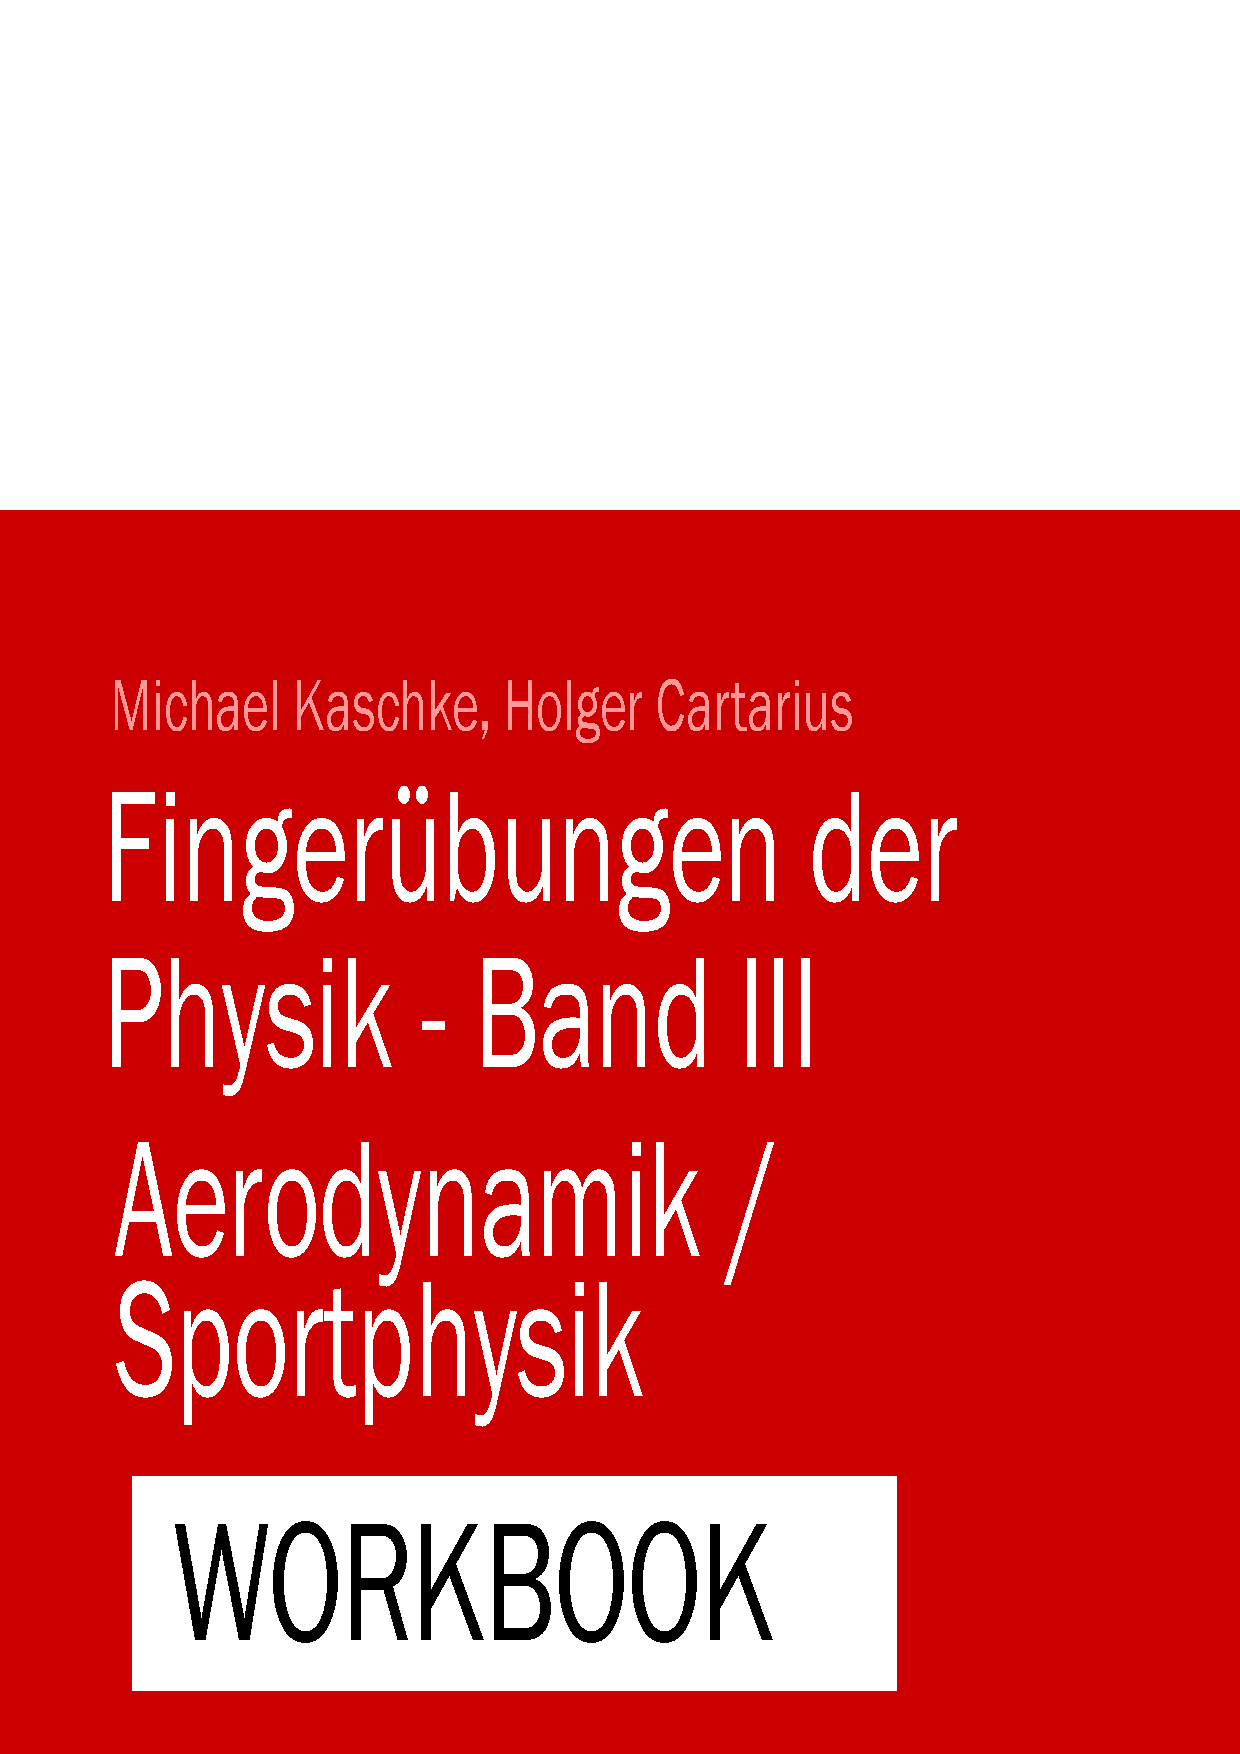
\includegraphics{BuchtitelseiteWB3.pdf}
%\end{textblock}
%\leavevmode
%\newpage 
%\thispagestyle{empty}
%\quad 
%\newpage
\pagestyle{fancy}

\author{Michael Kaschke und Holger Cartarius\\ \\
%unter Mitwirkung von Ulrich Potthoff
}
\title{Finger�bungen der Physik\\ \\
Band III \\ \\ Aerodynamik - Sportphysik \\ \\ Workbook\\}

\subtitle{Ein �bungsbuch zu im Studium selten behandelten Kapiteln der Physik mit ausf�hrlich dargestellten Problemen und \matlab-Programmen.}
\smallskip
\maketitle

\begin{dedication}
\;\;\;F�r alle Studenten und Studentinnen, die uns mit ihren neugierigen Fragen immer wieder
zeigen, dass es in der Physik auch in den kleinsten Nischen ganz viel zu entdecken gibt und \\
f�r alle, die Freude an der Sch�nheit und der gro�artigen Vielfalt der Physik gefunden haben oder vielleicht auch mit Hilfe dieses Buches f�r sich entdecken m�gen.\\
\textsc{Michael Kaschke und Holger Cartarius}\\ 
\medskip
\medskip
\medskip
F�r meine Frau \textsc{Sylvia} und meine Kinder \textsc{Johannes und Maria}, die mich jederzeit unterst�tzten und  mir immer viel Geduld und Verst�ndnis f�r meine vielen Projekte entgegen brachten.\\
\textsc{Michael Kaschke}\\
\medskip
\medskip
\medskip
F�r meine Eltern Hildegard und Rainer Cartarius, die mich jederzeit auf meinem Weg durch das Studium und die Anf�nge in der Wissenschaft unterst�tzten.\\
\textsc{Holger Cartarius}
\end{dedication}

\frontmatter%%%%%%%%%%%%%%%%%%%%%%%%%%%%%%%%%%%%%%%%%%%>

%\documentclass[makeidx,envcountchap,graybox,deutsch,ngerman,sectrefs]{svmono}
%\documentclass[envcountchap,graybox,deutsch,sectrefs]{svmono}
%%%%% eigene tempor�re Abk�rzungsliste, f�r die Zeit, bis einheitliche Schreibungen bestehen
\usepackage{tempshort}
%%  Von Springer empfohlene Pakete %% 
%%\documentclass[envcountsect,graybox,deutsch,sectrefs]{svmono}
\usepackage{chapterbib}
\usepackage{type1cm}
\usepackage[ansinew]{inputenc}
\usepackage{babel}
\usepackage[pdftex]{graphicx} %PDF-Vektorgrafiken einbinden
\usepackage{newtxtext} %Typischer Springer-Font
\usepackage{newtxmath}
\usepackage{multicol}
\usepackage[bottom]{footmisc} %Platziert alle Fu�noten unten  
\usepackage[nobreak]{cite}
%\usepackage{biblatex}
\usepackage{cancel}
\usepackage[absolute]{textpos}
\usepackage{graphicx}
\usepackage{pdfpages}

%\usepackage{floatrow}
%\usepackage{mwe}
\usepackage[figuresright]{rotating}
\usepackage{bigints}
\let\laplace\relax  % Vermeidung der Fehlermeldung "\laplace already defined."
\usepackage{trfsigns}
\usepackage{amsmath}
\usepackage{tabulary}
\usepackage{tabularx}

%%  Eigene Pakete %%
\usepackage{adjustbox}
\usepackage{wasysym}
\usepackage{gensymb}
\usepackage{float}
\usepackage{caption}
\usepackage[left=5cm,right=4cm,top=3cm,bottom=4cm,includeheadfoot]{geometry}

%\usepackage{wasysym}
%\usepackage{bigints}
%\usepackage{esint}
%\usepackage{relsize,exscale}

\usepackage{mathtools}   % Vermeidung der Fehlermeldung "Undefined control sequence \coloneqq."


% header and footer
\usepackage{fancyhdr}
\pagestyle{fancy}
\fancyhead[LE,RO]\thepage
\renewcommand{\sectionmark}[1]{\markright{\thesection.\ #1}}
%\fancyhead[LO]{\nouppercase\leftmark}
%\fancyhead[RE]{\nouppercase\rightmark}
\fancyhead[LO]{\nouppercase\rightmark}
\fancyhead[RE]{\nouppercase\leftmark}
\fancyfoot{}
% svmono hat offenbar irgendwas merkw�rdig definiert, darum mu� hier verbreitert werden
%\addtolength\headwidth{25pt}
\setlength{\headheight}{25pt}

%% Units
\usepackage{siunitx}
\sisetup{
  locale = US,
  per-mode = reciprocal, %symbol, % | reciprocal | fraction | ?
  exponent-product = \cdot,
  separate-uncertainty,
  %exponent-to-prefix,
  %prefixes-as-symbols = false,
  %list-units = brackets,% | single | repeat
  %range-units = brackets,% | single | repeat
  %multi-part-units = brackets,% | single | repeat
}
\usepackage{chngcntr}
\usepackage{booktabs}
\usepackage{slashed}
\usepackage{listings}
\usepackage{color} %red, green, blue, yellow, cyan, magenta, black, white
%\usepackage{color} %Einfache Farbendefinition -> von Graybox-Option ben�tigt
\usepackage{multirow}
\usepackage{longtable} %Tabellen �ber mehrere Seiten hinweg
\usepackage{framed} % von Graybox-Option ben�tigt
\usepackage[shortlabels]{enumitem} %Erweiterte Aufz�hloptionen
\usepackage{array}
\usepackage[xindy]{imakeidx} %Wortindex und Personenindex erstellen

\usepackage[hyphens]{url}
%\usepackage[breaklinks,colorlinks=true,linkcolor=black,urlcolor=blue,citecolor=black,filecolor=green,hyperfootnotes=false]{hyperref}
\usepackage[                                    %Hyperref erstellt ein Bookmark/Lesezeichen im PDF. siehe https://www.namsu.de/Extra/pakete/Hyperref.html
bookmarksopen=true,															%Das Lesezeichen ist ge�ffnet beim �ffnen der PDF.
bookmarksnumbered=true,                         %Zahlen werden im Bookmark angezeigt.   
plainpages=false,
pdfpagelabels,
colorlinks=true,                                %Links werden farbig dargestellt.
linkcolor=black, citecolor=black, urlcolor=cyan %Farben definieren.
]{hyperref}                                     %Sollte als letztes eingebunden werden, da es sehr viele Verweise und �nderungen erzeugt. Das Packet ist sehr stark, aber auch umfangreich ist. 

%\usepackage[breaklinks,colorlinks=true,linkcolor=black,urlcolor=blue,citecolor=black,filecolor=green,hyperfootnotes=false]{hyperref}
%\usepackage[breaklinks,colorlinks=true,linkcolor=black,urlcolor=blue,citecolor=black,filecolor=green,hyperfootnotes=false
            %pdftex,
            %pdfauthor={Kaschke, Cartarius},
            %pdftitle={Finger�bungen der Physik}
            %pdfsubject={Ein Repetitorium und �bungsbuch zu im Studium wenig behandelten Kapiteln der Physik mit ausf�hrlich behandelten Problemen und MATLAB-Programmen},
            %pdfkeywords={Physik, Mechanik}
            %]{hyperref}
\pdfminorversion=5

\usepackage{hypcap}
\usepackage[record,section=section,stylemods={mcols},automake]{glossaries-extra}
\usepackage{glossary-longextra}
%\usepackage{glossary-bookindex}
%\makeindex
\setglossarystyle{long-name-sym-desc-loc}
\setabbreviationstyle[acronym]{long-short}

\definecolor{killA}{rgb}{.7,.3,.3}
\newcommand\killA[1]{\bgroup\color{killA}{\cancel{#1}}\egroup}
\newcommand\killB[1]{\bgroup\color{cyan!30!black}{\cancel{#1}}\egroup}

% typographisch korrekte Abk�rzungen (needs to be loaded after hyperref)
\usepackage{abbrev}
\newglossary*{bew}{Glossar}
\newglossary*{hm}{Glossar}
\newglossary*{adyn}{Glossar}
\newglossary*{kontmech}{Glossar}
\newglossary*{aero}{Glossar}
\newglossary*{edyn}{Glossar}
\newglossary*{spo}{Glossar}
\newglossary*{optbas}{Glossar}
\newglossary*{optger}{Glossar}
\newglossary*{optatm}{Glossar}
\newglossary*{optspez}{Glossar}
\GlsXtrLoadResources[src={bew/gloss},type=bew]
\GlsXtrLoadResources[src={hm/gloss},type=hm]
\GlsXtrLoadResources[src={adyn/gloss},type=adyn]
\GlsXtrLoadResources[src={kontmech/gloss},type=kontmech]
\GlsXtrLoadResources[src={aero/gloss},type=aero]
\GlsXtrLoadResources[src={spo/gloss},type=spo]
\GlsXtrLoadResources[src={edyn/gloss},type=edyn]
\GlsXtrLoadResources[src={optbas/gloss},type=optbas]
\GlsXtrLoadResources[src={optger/gloss},type=optger]
\GlsXtrLoadResources[src={optatm/gloss},type=optatm]
\GlsXtrLoadResources[src={optspez/gloss},type=optspez]
\glssetcategoryattribute{bew}{indexname}{true}
%\renewcommand\index\newterm
%\newcolumntype{g}[1]{>{\RaggedRight\hspace{0pt}}p{#1}}
%\renewcommand\glslongextraNameAlign{g}
\renewcommand\glslongextraLocationAlign{@{\ ~\ }>{\raggedright}p{\glspagelistwidth}}
\definecolor{gls}{rgb}{.4,.4,.5}
\renewcommand*{\glstextformat}[1]{\textcolor{gls}{#1}}

%Absatzregeln
\clubpenalty = 30000 %Keine einzelnen Absatzzeilen
\widowpenalty = 30000
\setlength{\parindent}{0em} 
\newcolumntype{L}[1]{>{\raggedright\arraybackslash}p{#1}}
\newcolumntype{C}[1]{>{\centering\arraybackslash}p{#1}}
\newcolumntype{R}[1]{>{\raggedleft\arraybackslash}p{#1}}

\usepackage{xstring}

\newcommand\mfile[2]{%
\saveexpandmode\noexpandarg
\StrSubstitute{#2}{_}{\_}[\tmpname]
\restoreexpandmode
\href{MatlabDateien/\chapname/#1\tmpname}{\tmpname}}

%%% Hyperlinks zu MATLAB Dateien
%\newcommand\mlref[1]{\mfile{}{#1}}
%\newcommand\mlinclref[1]{\mfile{IncludeFolder/}{#1}}
%\newcommand\mldataref[1]{\mfile{Data/}{#1}}

%%% .. f�r ein Verzeichnis hoch
%%% . f�r aktuelle Verzeichnis
%% lokal: MatlabDateien/bew
%\newcommand\mlbewref[1]{\href{MatlabDateien/bew/#1}{#1}}
%% git: https://github.com/sn-code-inside/fingeruebungen-physik/tree/main/bew

\newcommand{\mlrefwithindex}[2]{%
  \index[mfiles]{#2}%   <-- Eintrag im M-File-Index mit aktueller Seitenzahl
  \href{https://github.com/sn-code-inside/fingeruebungen-physik/tree/main/#1/#2}{#2}%
}


%\newcommand\mlbewref[1]{\href{https://github.com/sn-code-inside/fingeruebungen-physik/tree/main/bew/#1}{#1}}
%\newcommand\mlbewdref[1]{\href{https://github.com/sn-code-inside/fingeruebungen-physik/tree/main/bew/Data/#1}{#1}}
%\newcommand\mlbewiref[1]{\href{https://github.com/sn-code-inside/fingeruebungen-physik/tree/main/bew/IncludeFolder/#1}{#1}}
%\newcommand\mlkontmechref[1]{\href{https://github.com/sn-code-inside/fingeruebungen-physik/tree/main/kontmech/#1}{#1}}
%\newcommand\mlkontmechdref[1]{\href{https://github.com/sn-code-inside/fingeruebungen-physik/tree/main/kontmech/Data/#1}{#1}}
%\newcommand\mlkontmechiref[1]{\href{https://github.com/sn-code-inside/fingeruebungen-physik/tree/main/kontmech/IncludeFolder/#1}{#1}}
%\newcommand\mlhmref[1]{\href{https://github.com/sn-code-inside/fingeruebungen-physik/tree/main/hm/#1}{#1}}
%\newcommand\mlhmdref[1]{\href{https://github.com/sn-code-inside/fingeruebungen-physik/tree/main/hm/Data/#1}{#1}}
%\newcommand\mlhmiref[1]{\href{https://github.com/sn-code-inside/fingeruebungen-physik/tree/main/hm/IncludeFolder/#1}{#1}}
%\newcommand\mladynref[1]{\href{https://github.com/sn-code-inside/fingeruebungen-physik/tree/main/adyn/#1}{#1}}
%\newcommand\mladyndref[1]{\href{https://github.com/sn-code-inside/fingeruebungen-physik/tree/main/adyn/Data/#1}{#1}}
%\newcommand\mladyniref[1]{\href{https://github.com/sn-code-inside/fingeruebungen-physik/tree/main/adyn/IncludeFolder/#1}{#1}}
%\newcommand\mledynref[1]{\href{https://github.com/sn-code-inside/fingeruebungen-physik/tree/main/edyn/#1}{#1}}
%\newcommand\mledyndref[1]{\href{https://github.com/sn-code-inside/fingeruebungen-physik/tree/main/edyn/Data/#1}{#1}}
%\newcommand\mledyniref[1]{\href{https://github.com/sn-code-inside/fingeruebungen-physik/tree/main/edyn/IncludeFolder/#1}{#1}}
%\newcommand\mloptbasref[1]{\href{https://github.com/sn-code-inside/fingeruebungen-physik/tree/main/optbas/#1}{#1}}
%\newcommand\mloptbasdref[1]{\href{https://github.com/sn-code-inside/fingeruebungen-physik/tree/main/optbas/Data/#1}{#1}}
%\newcommand\mloptbasiref[1]{\href{https://github.com/sn-code-inside/fingeruebungen-physik/tree/main/optbas/IncludeFolder/#1}{#1}}
%\newcommand\mloptspezref[1]{\href{https://github.com/sn-code-inside/fingeruebungen-physik/tree/main/optspez/#1}{#1}}
%\newcommand\mloptspezdref[1]{\href{https://github.com/sn-code-inside/fingeruebungen-physik/tree/main/optspez/Data/#1}{#1}}
%\newcommand\mloptspeziref[1]{\href{https://github.com/sn-code-inside/fingeruebungen-physik/tree/main/optspez/IncludeFolder/#1}{#1}}

\newcommand\mlbewref[1]{\mlrefwithindex{bew}{#1}}
\newcommand\mlbewdref[1]{\mlrefwithindex{bew/Data}{#1}}
\newcommand\mlbewiref[1]{\mlrefwithindex{bew/Include}{#1}}
\newcommand\mlkontmechref[1]{\mlrefwithindex{kontmech}{#1}}
\newcommand\mlkontmechdref[1]{\mlrefwithindex{kontmech/Data}{#1}}
\newcommand\mlkontmechiref[1]{\mlrefwithindex{kontmech/Include}{#1}}
\newcommand\mlhmref[1]{\mlrefwithindex{hm}{#1}}
\newcommand\mlhmdref[1]{\mlrefwithindex{hm/Data}{#1}}
\newcommand\mlhmiref[1]{\mlrefwithindex{hm/Include}{#1}}
\newcommand\mladynref[1]{\mlrefwithindex{adyn}{#1}}
\newcommand\mladyndref[1]{\mlrefwithindex{adyn/Data}{#1}}
\newcommand\mladyniref[1]{\mlrefwithindex{adyn/Index}{#1}}
\newcommand\mledynref[1]{\mlrefwithindex{edyn}{#1}}
\newcommand\mledyndref[1]{\mlrefwithindex{edyn/Data}{#1}}
\newcommand\mledyniref[1]{\mlrefwithindex{edyn/Index}{#1}}
\newcommand\mloptbasref[1]{\mlrefwithindex{optbas}{#1}}
\newcommand\mloptbasdref[1]{\mlrefwithindex{optbas/Data}{#1}}
\newcommand\mloptbasiref[1]{\mlrefwithindex{optbas/Include}{#1}}
\newcommand\mloptspezref[1]{\mlrefwithindex{optspez}{#1}}
\newcommand\mloptspezdref[1]{\mlrefwithindex{optspez/Data}{#1}}
\newcommand\mloptspeziref[1]{\mlrefwithindex{optspez/Include}{#1}}
\newcommand\mloptgerref[1]{\mlrefwithindex{optger}{#1}}
\newcommand\mloptgerdref[1]{\mlrefwithindex{optger/Data}{#1}}
\newcommand\mloptgeriref[1]{\mlrefwithindex{optger/Include}{#1}}
\newcommand\mloptatmref[1]{\mlrefwithindex{optatm}{#1}}
\newcommand\mloptatmdref[1]{\mlrefwithindex{optatm/Data}{#1}}
\newcommand\mloptatmiref[1]{\mlrefwithindex{optatm/Include}{#1}}



\newcommand\mlcmd[1]{\textcolor{cyan}{\texttt{#1}}}

%Grafikregeln
\graphicspath{{hm/graphs/}
	                    	{bew/graphs/}
     						{kontmech/graphs/}
							{hm/graphs/}
							{adyn/graphs/}
							{edyn/graphs/}
							{kontmech/graphs/}
							{spo/graphs/}
							{optbas/graphs/}
							{optger/graphs/}
							{optatm/graphs/}
							{solman/graphs/}
                                                        {aero/graphs}}
\DeclareGraphicsExtensions{.pdf, .png, .jpg, .jpeg}
\def\figname{Abb}
\newcommand\figref[1]{\figname.\ \ref{abb:#1}}
\usepackage[labelfont=bf]{caption}

\usepackage{tocloft}
\usepackage{etoc}
\setlength\cftfignumwidth{30pt}

% Flatterrand links
\cftsetindents{chapter}{0em}{4em}
\cftsetindents{section}{1.5em}{4em}
\cftsetindents{subsection}{3.8em}{4em}

% flacher Rand links
%\cftsetindents{chapter}{0em}{4em}
%\cftsetindents{section}{0em}{4em}
%\cftsetindents{subsection}{0em}{4em}

\newcommand\partitle[1]{
\addcontentsline{toc}{part}{#1}
\begin{titlepage}
  %\vskip 60%\p@
  \begin{center}
    {\LARGE Finger�bungen der Physik -- #1 \par}
    \vskip 3em%
    {\large Michael Kaschke und Holger Cartarius\par}
  \end{center}
\end{titlepage}
}

%\newcommand\mlref[1]{\href{\chapname/matlab/#1}{#1}}
%\newcommand\mlinclref[1]{\href{\chapname/matlab/IncludeFolder/#1}{\color{cyan}{#1}}}

%Neue Kommandos
\newcommand{\lk}{\left(}        %gro�e runde Klammer (links)
\newcommand{\rk}{\right )}      %gro�e runde Klammer (rechts)
\newcommand{\lgk}{\left \{}     %gro�e geschweifte Klammer (links)
\newcommand{\rgk}{\right \}}    %gro�e geschweifte Klammer (rechts)
\newcommand{\lek}{\left [}      %gro�e eckige Klammer (links)
\newcommand{\rek}{\right ]}     %gro�e eckige Klammer (rechts)
\newcommand{\anf}[1]{\glqq#1\grqq}    %Deutsche Anf�hrungszeichen: \anf{}
\newcommand{\defined}{:=}				%Definition
\newcommand{\curl}{\text{\textbf{rot}}\,}	%Rotation-Operator curl()
\newcommand{\ket}[1]{|#1\rangle}		%Quantenmechanischer Zustand
\newcommand{\curvelintri}{\,\overset{\blacktriangle}{\smallfrown}}
\newcommand{\straighttri}{\blacktriangle}
\newcommand{\UT}{\text{UT}}
\newcommand{\UTC}{\text{UTC}}
\newcommand{\JD}{\text{JD}}
\newcommand{\JDE}{\text{JDE}}
\newcommand{\MJD}{\text{MJD}}
\newcommand{\TDT}{\text{TDT}}
\newcommand{\TT}{\text{TT}}
\newcommand{\NVS}{\text{Navier-Stokes-Gleichungen}}
\newcommand{\MWG}{\text{Maxwell-Gleichungen}}
\newcommand{\EMW}{\text{Elektromagnetische Wellen}}
\newcommand{\eMW}{\text{elektromagnetischen Wellen}}
\newcommand{\RT}{\text{Relativit�tstheorie~}}
\newcommand{\au}{\mathrm{AE}}
\newcommand{\ET}{\text{ET}}
\newcommand{\TAI}{\text{TAI}}
\newcommand{\GMST}{\text{GMST}}
\newcommand{\LMST}{\text{LMST}}
\newcommand{\MESZ}{\text{MESZ}}
\newcommand{\KOS}{\text{Koordinatensystem }}
\newcommand{\DGL}{\text{Differentialgleichung }}
\newcommand{\NA}{\text{NA}}
\newcommand{\uA}{\text{u}}  %atomare Masseneinheit
\newcommand{\MOZ}{\text{MOZ}}
\newcommand{\grad}{\text{\textbf{grad}}\,}	%Gradient-Operator grad()
\newcommand{\uproman}[1]{\mathrm{\uppercase\expandafter{\romannumeral#1}}}
\newcommand{\lowroman}[1]{\romannumeral#1\relax}

\newcommand\todo[1]{\textcolor{red}{TODO: #1}}

\renewcommand{\=}[1]{\stackrel{\text{#1}}{=}}  %Schrift �ber Gleich-Zeichen
\renewcommand{\d}{\partial}
\newcommand{\lra}{\Leftrightarrow}  %�quivalenz-Pfeile
\newcommand{\abs}[1]{\left\vert#1\right\vert}     %Betragsklammern
\renewcommand{\Re}{\mathrm{Re}}                          %Realteil
\renewcommand{\Im}{\mathrm{Im}}                          %Imagin�rteil
\renewcommand{\im}{\mathrm{i}}                         %Imagin�re Einheit
\renewcommand{\epsilon}{\varepsilon} 
\newcommand{\keff}{k_\text{eff}}
\newcommand{\con}{\text{const}}
\newcommand{\conv}{\vec{const}}
\newcommand{\PL}{\mathcal{P}_}
\newcommand{\artanh}{\mathrm{artanh}}
% QED-Symbol im text- bzw. Mathemodus
\newcommand{\textqed}{\hfill ~ $\square$}
\newcommand{\mmqed}{\tag*{$\square$}}

\newcommand{\fa}{(\textbf{a}) }
\newcommand{\fb}{(\textbf{b}) }
\newcommand{\fc}{(\textbf{c}) }
\newcommand{\fd}{(\textbf{d}) }
\newcommand{\fe}{(\textbf{e}) }
\newcommand{\ff}{(\textbf{f}) }

\newcommand{\iF}{im Folgenden~}
\newcommand{\iA}{im Allgemeinen~}


\DeclareMathOperator\divv{div}
\DeclareMathOperator\res{Res}
\DeclareMathOperator{\sech}{sech}
\DeclareMathOperator\sgn{sgn}

% f�r Appendix - MATLAB Referenz
\newcommand{\rotv}{\vec{rot}\,}
\newcommand{\gradv}{\vec{grad}\,}
\newcommand{\nablav}{\vec{\nabla}\,}

\newcommand{\ceil}{\mathrm{ceil}}
\newcommand{\sinc}{\mathrm{sinc}}
\newcommand{\diag}{\mathrm{diag}}
\newcommand{\sign}{\mathrm{sign}}
\newcommand{\length}{\mathrm{length}}
\newcommand{\sort}{\mathrm{sort}}
\newcommand{\summ}{\mathrm{sum}}
\newcommand{\asin}{\mathrm{asin}}
\newcommand{\acos}{\mathrm{acos}}
\newcommand{\atan}{\mathrm{atan}}
\newcommand{\prodd}{\mathrm{prod}}
\newcommand{\median}{\mathrm{mediab}}
\newcommand{\mean}{\mathrm{mean}}
\newcommand{\std}{\mathrm{std}}
\newcommand{\eye}{\mathrm{eye}}
\newcommand{\zeros}{\mathrm{zeros}}
\newcommand{\ones}{\mathrm{ones}}
\newcommand{\rand}{\mathrm{rand}}
\newcommand{\inline}{\mathrm{inline}}
\newcommand{\modd}{\mathrm{mod}}
\newcommand{\floor}{\mathrm{floor}}
\newcommand{\round}{\mathrm{round}}
\newcommand{\rem}{\mathrm{rem}}
\newcommand{\sqrtt}{\mathrm{sqrt}}
\newcommand{\triu}{\mathrm{triu}}
\newcommand{\tril}{\mathrm{tril}}
\newcommand{\size}{\mathrm{size}}
\newcommand{\dett}{\mathrm{det}}
\newcommand{\inv}{\mathrm{inv}}
\newcommand{\rank}{\mathrm{rank}}
\newcommand{\rref}{\mathrm{rref}}
\newcommand{\eig}{\mathrm{eig}}
\newcommand{\poly}{\mathrm{poly}}
\newcommand{\lu}{\mathrm{lu}}
\newcommand{\qr}{\mathrm{qr}}
\newcommand{\quaddd}{\mathrm{quad}}
\newcommand{\fzero}{\mathrm{fzero}}
\newcommand{\roots}{\mathrm{roots}}
\newcommand{\odezd}{\textcolor{mygreen}{\texttt{ode23}}}
\newcommand{\odevf}{\textcolor{mygreen}{\texttt{ode45}}}
\newcommand{\odeeds}{\textcolor{mygreen}{\texttt{ode13s}}}
\newcommand{\odeefs}{\textcolor{mygreen}{\texttt{ode15s}}}
\newcommand{\ddezd}{\textcolor{mygreen}{\texttt{dde23}}}
\newcommand{\onlineZ}{online verf�gbaren Zusatzmaterialien{}}
\newcommand{\MKc}{\url{https://www.fingeruebungen-physik.de}{}}
\newcommand{\linklsg}{\href{https://www.fingeruebungen-physik.de}{\textcolor{blue} {$\rightarrow$ L�sungsteil.}}}
\newcommand{\githubSN}{\url{https://github.com/sn-code-inside/fingeruebungen-physik}{}\,\,}

\newcommand{\FT}{\mathcal{F}} %Fourier-Transformierte

% Aufz�hlung der L�sungen der Teilaufgaben
\newlist{subprobs}{enumerate}{1}
\setlist[subprobs]{
  label= \textbf{\textit{Teilaufgabe}} \textbf{\textit{\arabic*:}} \protect\thissubprob,
  ref=\arabic*, itemsep=\baselineskip, align=left}
\newcommand{\subprob}[1]{
  \def\thissubprob{\textbf{\textit{#1}}}\item ~\vspace{0.2\baselineskip} \newline}

\renewenvironment{example}[1]{
\refstepcounter{example}\par\medskip
\begin{shaded} 
\begin{samepage}
\noindent \textbf{\textit{Beispiel~\theexample: {#1}}}\\ 
\noindent{\color{black} \rule{\textwidth}{0.2 mm}}
\end{samepage}
}{\end{shaded}
\noindent{\color{black} \rule{\textwidth}{0.2 mm}}
} % or snugshade
\definecolor{shadecolor}{gray}{0.95}
\definecolor{mygreen}{RGB}{28,172,0} % color values Red, Green, Blue
\definecolor{mylilas}{RGB}{170,55,241}

\newenvironment{infobox}[1]{
     \begin{shaded} 
     \begin{samepage}
\noindent{\color{black} \rule{\textwidth}{0.2 mm}}
     \end{samepage}
}{\end{shaded}
\noindent{\color{black} \rule{\textwidth}{0.2 mm}}
} 
\definecolor{shadecolor}{gray}{0.95}
\definecolor{mygreen}{RGB}{28,172,0} % color values Red, Green, Blue
\definecolor{mylilas}{RGB}{170,55,241}


\newenvironment{nebenrechnung}[1]{
\begin{shaded} 
\begin{samepage}
\noindent\textbf{Nebenrechnung: \\} 
\noindent{\color{black} \rule{0.1\columnwidth}{0.2mm} \\}
\end{samepage}
}{\end{shaded}
\noindent{\color{black} \rule{0.1\columnwidth}{0.2mm} \\}
} % or snugshade
\definecolor{shadecolor}{gray}{0.95}
\definecolor{mygreen}{RGB}{28,172,0} % color values Red, Green, Blue
\definecolor{mylilas}{RGB}{170,55,241}

\newenvironment{merksatz}[1]{
\begin{shaded} 
\begin{samepage}
\noindent\textbf{Merke:\\} 
\noindent{\color{black} \rule{0.9\columnwidth}{0.2mm} \\ \\}
\end{samepage}
}{\end{shaded}
\noindent{\color{black} \rule{0.9\columnwidth}{0.2mm} \\}
} % or snugshade


\lstset{language=Matlab,%
    %basicstyle=\color{red},
    %basicstyle={\linespread{0.9}\ttfamily},
    basicstyle=\footnotesize\ttfamily,
    breaklines=true,%
    morekeywords={matlab2tikz},
    keywordstyle={\small \color{mygreen}},%
    morekeywords=[2]{1}, keywordstyle=[2]{\small\color{black}},
    identifierstyle={\small \color{black}},%
    stringstyle={\small\color{mylilas}},
    commentstyle={\small\color{mylilas}},%
    showstringspaces=false,%without this there will be a symbol in the places where there is a space
    numbers=left,%
    numberstyle={\tiny \color{black}},% size of the numbers
    numbersep=9pt, % this defines how far the numbers are from the text
    emph=[1]{for,end,else,break, function},emphstyle=[1]\small \color{blue}, %some words to emphasise
    emph=[2]{odeset},emphstyle=[2]\small \color{mygreen}, %some words to emphasise
    %emph=[2]{word1,word2}, emphstyle=[2]{style},    
}

%\bibliographystyle{spphys.bst}

%Trennregeln f�r spezielle Worte
%\hyphenation{Fresnel \matlab �qui-nok-ti-um}

\DeclareSIUnit\erg{erg}
\DeclareSIUnit\cal{cal}
\DeclareSIUnit\celsius{C}
\DeclareSIUnit\m{M}
\DeclareSIUnit\kel{K^{-4}}

%Stichwort- und Personenverzeichnis
\makeindex[title=Stichwortverzeichnis] % Create the default index
\makeindex[name=personen,title=Personenverzeichnis] % Create an index named 'personen'
\newcommand{\indexp}[1]{\index[personen]{#1}}
\makeindex[name=mfiles,title=MATLAB-Skriptverzeichnis,columns=2]

% list of exercises
\newcommand{\loxname}{\Large �bungsverzeichnis}  % einheitliche Gr��e Large
\newlistof[chapter]{prob}{lox}\loxname
\newcommand\uebung[3][]{\label{prob:#2}%
\addcontentsline{lox}{prob}{\protect\numberline{}{\probRef{#2}:~#3#1}}%
\textbf{#1#3}\\[\baselineskip]}
\makeatletter
\renewcommand{\l@prob}{\@dottedtocline{1}{0em}{0em}}
\makeatother

\newcommand\einfach{\uebung[~$\ast$~~]}
\newcommand\mittel{\uebung[~$\ast\,\ast$~~]}
\newcommand\schwierig{\uebung[~$\ast\,\ast\,\ast$~~]}
\newcommand\zusatz{\uebung[~$\ast\,\ast\,\ast\,!$~~]}
%\newcommand\einfach{\uebung[~\textbf{*}~~]}
%\newcommand\mittel{\uebung[~\textbf{*\,*}~~]}
%\newcommand\schwierig{\uebung[~\textbf{*\,*\,*}~]}
%\newcommand\zusatz{\uebung[~\textbf{*\,*\,*\,!}~~]}
\usepackage[atend]{bookmark}
%\BookmarkAtEnd{%
%\bookmarksetup{startatroot}\bookmark[level=0,named=\loxname]{}}

\newcommand\kapitel[1]{Kapitel \ref{kap:#1}}
%\newcommand\kap[1]{Kap.\ \ref{kap:#1}}
\newcommand\kap[1]{Kap. \ref{kap:#1}}

\begin{document}
% customize prob and sol in svmono
\makeatletter
%\counterwithin*{chapter}{part}

\spn@wtheorem{prob}{\bgroup\exercisename\egroup}{\bfseries}{\rmfamily}
\makeatother
\renewenvironment{sol}[1]{\par\addvspace{6pt}\noindent\phantomsection{\textbf{L�sung \ref{#1}}} \ignorespaces}{\par\addvspace{6pt}}
\newcommand\probRef[1]{�bung \ref{prob:#1}}
\renewcommand\probref[1]{\textbf{\probRef{#1}}}
\newcommand\lsgref[1]{L�sung \ref{lsg:#1}}

\newcommand\sbullet[1][.5]{\mathbin{\vcenter{\hbox{\scalebox{#1}{$\bullet$}}}}}

\setcounter{table}{0}


%%%%%%%%%%%%%%%%%%%%%%%%%%%%%%%%%%%%%%%%%%%%%%%%%%%%%%%%%%%%%%%
\begingroup
\let\cleardoublepage\relax
\chapter*{Vorwort}

\begin{figure}
	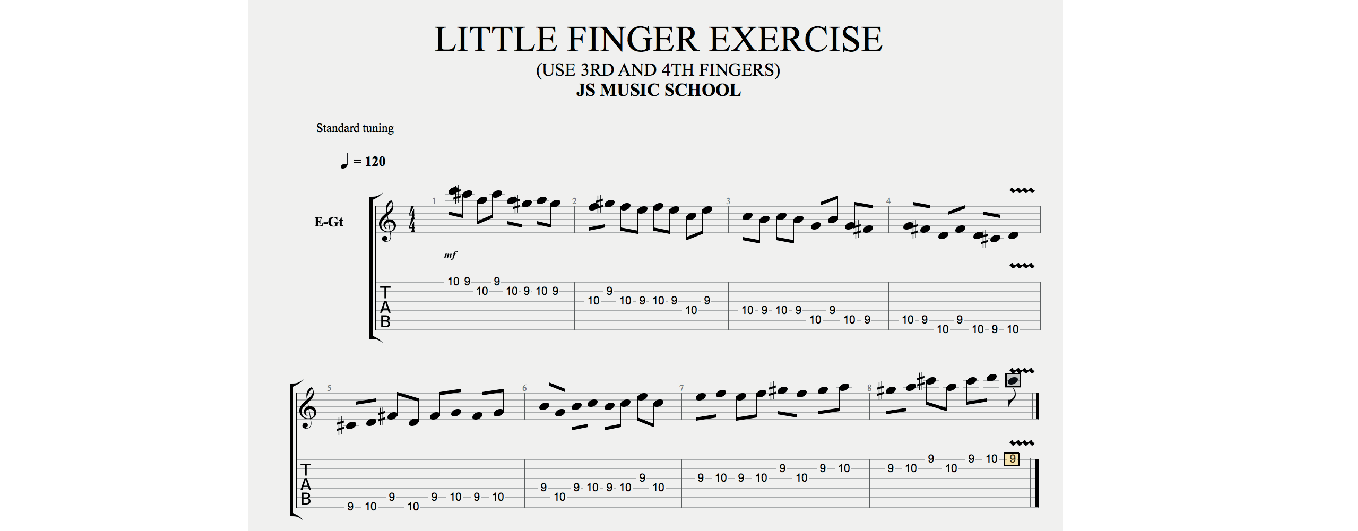
\includegraphics[width=\textwidth]{FingerExcercise.pdf}
%\caption{Finger�bungen}%
	\label{fig:FingerExcercise}
\end{figure}
Nach der positiven Aufnahme unseres bisherigen B�nde "`Finger�bungen der Physik"' legen wir hiermit mit der gleichen Intention den Band III vor. 
F�r einen Physiker\footnote{Die im Text verwendeten Formen des generischen Maskulinums (\zb \anf{Physiker}, \anf{Studenten}, \anf{Leser}) \usw schlie�en alle anderen Geschlechtsformen (\zb  \anf{Physikerin}, \anf{Studentin} \usw) ausdr�cklich mit ein.} gilt dasselbe wie f�r einen Pianisten: �bt dieser nicht st�ndig, wird auch die Hand eines Starpianisten irgendwann nicht mehr die Meisterwerke fl�ssig spielen k�nnen. Und nat�rlich macht es am meisten Spa�, St�cke zu spielen, die interessant und herausfordernd sind.\\

\textcolor{red}{\todo �berarbeiten}

%\textcolor{red}{
%Bei uns geh�ren in diesem Band die Fliegen Segeln und Sport, die im Curriculum des Physikstudiums eher selten oder oft nur wenig ausf�hrlich behandelt werden. Das sind aber gerade Themen, die viele Physikstudenten besonders interessieren, vielleicht sogar urspr�nglich die Motivation f�r die Aufnahme eines Studiums der Physik waren. 
%Es sind auch Bereiche, die sehr oft in den Leistungskursen der Physik/Naturwissenschaften in den Gymnasien behandelt werden und auch dort oft bestimmend f�r die Stimulation und Motivation der Sch�ler f�r die Naturwissenschaften sein k�nnen. Wie kaum ein anderes Gebiet geeignet sind diese beiden Gebiete auch geeignet, die Sch�nheit der Physik zu erfassen und zu vermitteln.\\
%Obwohl sich unsere Reihe prim�r an Studenten und Doktoranden der Physik, Mathematik und Ingenieurswissenschaften richtet, haben wir deshalb in diesem Band bewusst auch die Zielgruppe des Lehramts f�r naturwissenschaftliche F�cher im Blickfeld gehabt und hoffen, dass diese in diesem Buch 
%einen Fundus an �bungen, Beispielen und Anregungen f�r sich und f�r Problemstellungen und Projekte f�r Ihre Sch�ler gewinnen m�gen.
%Wir haben auch aus diesem Grund in weiten Teilen dieses Bands das Grundlagenwissen etwas unterhalb des Bachelors Physik angesetzt. Das Wissen aus Band I ist hilfreich, aber nicht notwendig f�r das Verst�ndnis dieses Bandes, der sich wiederum gleicherma�en zum Selbststudium wie auch zur Begleitung in Tutorien/�bungen eignet.
%Die hier vorgestellte Himmelsmechanik und Astrodynamik sind als in sich weitgehend abgeschlossene Kapitel konzipiert und leiten in die vertiefenden �bungen mit und ohne Computer ein. Wie im Band I sind die theoretischen Grundlagen im Sinne eines Repetitoriums zun�chst zusammengefasst. Diese Zusammenfassung kann und soll kein vollst�ndiger Ersatz f�r ein Lehrbuch und eine tiefere Einarbeitung sein, weswegen wir auch immer auf entsprechende weiterf�hrende Lehrb�cher verweisen.\\}

%\textcolor{red}{
%Wie im Band I (Mechanik) ausf�hrlich dargelegt, sind wir der festen �berzeugung, dass die heute Studierenden im Rahmen ihres Fachstudiums vielf�ltige numerische Methoden kennenlernen und praktische Erfahrungen damit sammeln m�ssen. Deswegen liegt gerade in diesen Gebieten der Himmelsmechanik und Astrodynamik ein Schwerpunkt auf der numerischen Berechnung der behandelten physikalischen Ph�nomene und Beispiele. Wir stimmen auch mit Rubin Landau (Am. J. Phys., \textbf{76}, 296-306 (2008)) �berein, der bereits 2008 argumentierte, dass Computermethoden neben Theorie und Experiment einen dritten \anf{Pfad} der physikalischen Erkenntnis darstellen und dass computergest�tzte Physik als eine Synthese von Physik, angewandter Mathematik und Informatik zu verstehen sei. Dennoch muss immer die physikalische Modellierung und analytischen Beschreibung der Probleme im Vordergrund stehen. Diese stellen wir deshalb der numerischen Berechnung stets voran.\\
%Es gibt mittlerweile eine Reihe sehr guter B�cher f�r Studenten zur computergest�tzten Physik auf Basis der Programmiersprache \textbf{\textit{Python}}. Wir haben uns aber weiterhin wie der Untertitel des Buches schon sagt, f�r \matlab{} entschieden, weil es in weiten Teilen der Industrie und der Forschung die Standardsoftware darstellt. \matlab{} ist hervorragend zur L�sung vieler mathematischer, physikalischer und technischer Probleme und zur grafischen Darstellung der Ergebnisse geeignet. Die akademische Bindung ist durch relativ preisg�nstige Studentenversionen bis heute erhalten geblieben und ist auch ein Grund f�r den gro�en Erfolg und die weite Verbreitung der Software. Ferner gibt es eine sehr gute Plattform \matlab{} Central (\url{https://de.mathworks.com/matlabcentral/}), die einen offenen Austausch f�r die Community der \matlab-Benutzer bietet und viele Programmpakete zum Download bereith�lt. Es gibt zahlreiche gute Einf�hrungen besonders f�r Physiker und Ingenieure in die Programmierung mit \matlab{}. Hinweise finden sich im Literaturverzeichnis.\\
%Prinzipiell spricht aber nichts dagegen, auf andere Softwarepakete zur�ckzugreifen, die �bertragung der \mscr e stellt \ia kein Problem dar. 
%\textbf{\textit{GNU Octave}}\index{GNU Octave} (\url{https://octave.org/}) ist vermutlich die beste Alternative zu \matlab. Octave l�uft auf Linux, Windows, und Mac. F�r viele Projekte ist ein \mscr{} auch unter GNU Octave ohne gro�e Modifikationen lauff�hig. Die Funktionskompatibilit�t von GNU Octave zur Basisversion von \matlab{} (ohne Toolboxen) ist weitgehend gegeben. Der Source Code von GNU Octave kann von der GNU Website heruntergeladen werden. \\
%\textbf{\textit{Python}}\index{Python} (\url{https://www.python.org/}) ist wie erw�hnt eine universelle Programmiersprache. Mit ihr l�sst sich �hnlich wie mit \matlab{} gut lesbarer, teils auch recht knapper Code erzeugen, der in seiner Struktur sehr �hnlich zu \matlab{} ist.
%Die Sprache ist mittlerweile in vielen L�ndern Teil des Curriculums an Schulen und Hochschulen. Python unterst�tzt die objektorientierte und die funktionale Programmierung, und kann auch wie \matlab{} als Skriptsprache genutzt werden.
%%NumPy und SciPy sind die zu Python geh�rigen Hauptpakete f�r das wissenschaftliche Rechnen. 
%Die Handhabung ist damit vergleichbar zu \matlab.
%%Die Integration von NumPy in Python erm�glicht die Verwendung und Kombination mit vielen weiteren Paketen aus dem umfangreichen Python-Umfeld. 
%Die Sprache und die wissenschaftlichen Programmpakete sind f�r Linux, Windows, und Mac OS X verf�gbar. 
%%Sehr empfehlenswert f�r Physiker und Ingenieure sind die Einf�hrungen in die Programmierung mit Python in \cite{Natt2020, Landau2015, Landau2007}.\\
%Ansonsten verweisen wir auf unsere Ausf�hrung zur computergest�tzten Physik im Band I und in den \onlineZ.}

Ein solches mehrb�ndiges Projekt ist ohne die Hilfe vieler Menschen nicht zu realisieren. 
Es ist hier unm�glich allen zu danken.\\

Ganz besonderer Dank aber geb�hrt unserem Koautor der \onlineZ, Herrn Dr. Ulrich Potthoff, f�r seine wertvolle Mitarbeit bei den L�sungen und den \matlab-Programmen. Ohne ihn w�re insbesondere der Umfang des Arbeitsbuches, in welchem umfangreiche L�sungsvorschl�ge inklusive der zugeh�rigen \matlab-Programme zusammengefasst sind, nicht m�glich gewesen. Sein sorgf�ltiges und kritisches Korrekturlesen, sowie umfangreiche Kontrollrechnungen und \matlab-Implementierungen haben viele wertvolle Verbesserungen erbracht.\\
Herrn Dr. Johannes Kaschke verdanken wir viele wertvolle Diskussionen und Anregungen zur \matlab-Programmierung. Frau Sylvia Kaschke hat uns nicht nur bei der Erstellung vieler Abbildungen, sondern auch moralisch bei manchen Durststrecken und mit vielen Fragen und Diskussionen unterst�tzt.\\
Ebenso geb�hrt besonderer Dank Herrn Dr. Michael Rill f�r die vielen Diskussionen und die Unterst�tzung bei der Erstellung der LaTeX-Dateien sowie vieler Abbildungen.\\
Dr. Andreas Dorsel, Dr. Rudolf von B�nau, Bernd Geh, Dr. Michael Kempe, Dr. Johannes-Maria Kaltenbach und vielen anderen sind wir f�r zahlreiche Anregungen und Diskussionen sehr dankbar.\\
Besonderer Dank geb�hrt auch dem Springer Verlag und hier vor allem Frau Dr. Gabriele Ruckelshausen und Herrn Ramkumar Padmanaban f�r die gute Zusammenarbeit und die vielen wertvollen Hinweise.\\

Ohne die Studenten und Studentinnen, an die sich das Buch ja vornehmlich richtet -- genannt seien besonders Jan Albicker, Kenneth von B�nau, Lennart Hoffmann, Paul Pitzel, Hauke Rehr, Philipp Simon, Juliane Vetter und Anne Weber -- w�re das Projekt nicht zu Ende gekommen. Ihnen allen gilt unser herzlicher Dank.\\

Wir w�nschen uns, dass auch dieser Band einen breiten Leserkreis findet und dass besonders auch Dozenten, Tutoren und Lehrer viele Anregungen f�r weiterf�hrende �bungen und Projektarbeiten in diesem Buch finden. Die online unter den Links \MKc{} \bzw \githubSN zur Verf�gung gestellten Materialien sollen gerade auch Projektarbeiten erm�glichen.\\ 


\textsc{Michael Kaschke, Holger Cartarius, Michael Kempe udn  (2026)}



%%%%%%%%%%%%%%%%%%%%%%%%%%%%%%%%%%%%%%%%%%%%%%%%%%%%%%%%%%%%%%%%%%%%%%%%%%%%%%%%%%%%%%%%%%%%%%%%%%%%%%%%%%%%%
%%%%%%%%%%%%%%%%%%%%%%%%%%%%%%%%%%%%%%%%%%%%%%%%%%%%%%%%%%%%%%%%%%%%%%%%%%%%%%%%%%%%%%%%%%%%%%%%%%%%%%%%%%%%%

\chapter*{Ausz�ge aus dem Vorwort zum Band I}

\subsection*{Wie kam es zur Idee f�r dieses Buch?}

An der Universit�t Jena kursierte vor etlichen Jahren unter uns Studenten 
der folgende Witz: F�r Absolventen der Universit�t ist ein Wettbewerb ausgeschrieben, bei dem es gilt einen Projektvorschlag f�r die Erstellung eines Melkkarussells zu machen und ein Modell vorzustellen.
Nach einiger Zeit werden der Kommission drei Arbeiten eingereicht, die eines Maschinenbau-Ingenieurs, die eines Betriebswirtschaftlers und die eines Physikers.
Der Ingenieur kommt mit einem perfekt funktionierenden 1:10-Modell und einer langen Liste technischer Parameter.
Die Kommission ist beeindruckt.
Der Betriebswirtschaftler pr�sentiert Kostenrechnungen, eine Trendanalyse des Milchpreises und vor allem eine �berzeugende Gewinnberechnung.
Begeistert davon erwartet die Kommission den dritten Bewerber.
Der Physiker kommt nur mit einem St�ck Kreide, geht an die Tafel, malt einen Kreis und sagt: \glq{}Als Modell habe ich die Kuh als Kugel und die Milch als homogen verteilt angenommen.
Daraus ergibt sich folgende Differentialgleichung ...\grq{}.

Uns gef�llt der Witz noch heute, beschreibt er doch treffend, wozu die Physikausbildung bef�higt: Abstraktion, Modellbildung, und die Ableitung von Prinzipien, um auf deren Basis eine geeignete mathematische Beschreibung und damit eine Erkl�rung von Ph�nomenen zu finden.
Charakteristika, auf die der Physiker zurecht stolz ist und die den geradezu legend�ren Ruf seiner universellen Einsetzbarkeit begr�nden.
Allerdings haben Physiker w�hrend des Studiums -- abgesehen vielleicht vom physikalischen Praktikum -- wenig Gelegenheit und Zeit, konkrete Problemstellungen aus dem Alltag detailliert zu berechnen und damit experimentell verifizierbar zu machen.
Gern behilft sich der Physiker dann mit den sogenannten \anf{back of the envelope}-Rechnungen%
\footnote{Siehe die B�cher von C. Swartz, Back-of-the-Envelope Physics (The Johns Hopkins University Press, Baltimore,
2003), S. Mahajan, The Art of Insight in Science and Engineering (The MIT Press, Cambridge, 2014) und A. Zee, Fly by Night Physics: How Physicists Use the Backs of Envelopes (Princeton
University Press, Princeton, 2020)}, um eine Absch�tzung zu erhalten.
Wir sind ebenfalls gro�e Anh�nger dieser Methode, da sie oft den ersten Zugang zum Verst�ndnis eines physikalischen Problems darstellt.
Allerdings ist es immer schade, wenn weder Zeit noch Methodik zur Verf�gung stehen, solch faszinierende Probleme wie \zb den Fehlgang einer Pendeluhr, die Dauer eines Fallschirmsprungs aus der Stratosph�re, die genaue Farbverteilung in einem Regenbogen oder einem Halo genau zu berechnen.
Nat�rlich kann jeder Physiker diese Ph�nomene erkl�ren, ebenso wie eine Sonnenfinsternis oder die grunds�tzliche Physik des Segelns.
Aber kann er auch die genaue Uhrzeit und den Ort der Sonnenfinsternis berechnen oder die Maximalgeschwindigkeit eines Segelbootes?
Mit diesem Buch wollen wir eine Auswahl \emph{sch�ner} Physikprobleme behandeln.
Dabei ist uns bewusst, dass das Kriterium der Sch�nheit immer ein subjektives Empfinden beinhaltet.
Es sind aber vor allem aber Themen, die sonst selten oder wenig ausf�hrlich behandelt werden.
Wir schauen dabei auf ganz verschiedene physikalische Bereiche und Ph�nomene, die vielleicht auch den Nichtphysiker interessieren und deren Berechnung und Erkl�rung dem Physiker erlauben, die Sch�nheit der Physik zu erfassen und auch anderen zu vermitteln.

Ziel des Buches ist es, anhand in sich abgeschlossener Kapitel diese ausgew�hlten einzelnen physikalischen Probleme, Ph�nomene oder auch nur Alltagsthemen so zu behandeln, dass sowohl das physikalische Grundverst�ndnis vermittelt und gesch�rft wird, als auch eine m�glichst genaue und detaillierte quantitative Analyse und numerische Berechnung auf dem Computer durchgef�hrt werden kann.
Mit diesen kann dann der Physiker beim oben beschriebenen Wettbewerb auch mit seinen Konkurrenten in Bezug auf Detail und Realit�tsn�he mithalten. 

\subsection*{F�r wen ist dieses Buch gedacht?}

Ganz einfach gesagt richtet es sich an alle, die Freude an der Physik haben und diese auch f�r allseits interessierende Probleme und Fragestellungen anwenden wollen.
Prim�r adressiert es Studierende und Doktoranden der Physik, Mathematik und Ingenieurswissenschaften ebenso wie des Lehramtes f�r naturwissenschaftliche F�cher.
Genauso ist es f�r Dozenten und Lehrer der Physik gedacht, die aus dem Fundus der �bungen und Beispiele Anregungen f�r eigene Problemstellungen und Projekte gewinnen m�gen.
Die Physik, wie sie im Studium zum Bachelor-Abschluss erreicht wird, stellt in etwa die Grundlage dar, auf der das Buch aufbaut.
Es eignet sich gleicherma�en zum Selbststudium wie zur Benutzung in Tutorien/�bungen.
Es ist nicht als eigentliches Lehrbuch gedacht. Die einzelnen Kapitel sind aber in sich geschlossen und k�nnen daher als Repetitorium und Kurzusammenfassung verstanden werden, sie leiten im Allgemeinen in die vertiefenden �bungen ein. .

Wir haben es als \anf{Finger�bungen der Physik} betitelt.
F�r einen Physiker gilt dasselbe wie f�r einen Pianisten: �bt dieser nicht st�ndig, wird auch die Hand eines Starpianisten irgendwann nicht mehr die Meisterwerke fl�ssig spielen k�nnen.
Mit Finger�bungen der Physik ist gemeint, dass wir das gesamte Handwerkszeug des Physikers wie Modellbildung, Analysis und Algebra, Absch�tzungen, St�rungsrechnungen usw. benutzen wollen, um damit spannende und interessante physikalische Alltagsprobleme zu erkl�ren und quantitativ zu beschreiben.

\subsection*{Warum gerade diese Auswahl der Themen?}

Jede Auswahl ist subjektiv.
Dennoch haben wir versucht, bei der Auswahl auch objektive Kriterien einflie�en zu lassen. Die Probleme und Ph�nomene
\begin{enumerate}
	\item sollen sich sinnvoll zu gr��eren Kapiteln b�ndeln lassen.
          Diese sind wiederum in sich relativ geschlossen und werden durch eine Zusammenfassung der grundlegenden Theorie eingef�hrt.
	\item erlauben eine schrittweise Erl�uterung, Einf�hrung oder auch Wiederholung der zugrundeliegenden Theorie.
	\item sind allgemein bekannt oder k�nnen zumindest zu verwandten Problemen in Bezug gesetzt werden.
	\item werden selten oder nur oberfl�chlich im Physik-Studiengang (bis zum Bachelor) behandelt.
        \item k�nnen gut in \matlab{} oder anderen Programmiersprachen wie GNU Octave oder Python bearbeitet werden und erlauben die Berechnung nachpr�fbarer Ergebnisse.
	\item bieten eine Basis f�r weitere und tiefergehende Fragestellungen und �bungen.
\end{enumerate}

\subsection*{Warum numerische Berechnungen und \matlab?}

Wir sind der �berzeugung, dass numerische Verfahren zur L�sung realit�tsnaher Problemstellungen unverzichtbar sind. Diese werden aber ebenso wie die oben genannten \anf{seltenen} Kapitel in der Lehre und in B�chern kaum behandelt.
Hingegen beobachtet man in letzter Zeit im Internet eine Flut von Apps, die mehr oder weniger fertige Darstellungen und durchaus graphisch ansprechende Simulationen von physikalischen Vorg�ngen und Ph�nomenen zeigen. Sie erzeugen daher sicher eine gute Anschaulichkeit und auch ein gutes Grundverst�ndnis. Sie erlauben h�ufig mit einigen interaktiven Elementen auch eine gewisse spielerische Simulationsbandbreite, erm�glichen aber fast nie einen Einblick in die zugrundeliegenden Algorithmen.
Daher halten wir das Konzept, Grundlagenthemen der Physik anhand spannender realit�tsnaher Beispiele und Probleme zu erl�utern und mit numerischen Methoden zu verbinden, f�r sehr wichtig.\\
%In den nachfolgenden \anf{Bemerkungen zur computergest�tzten Physik} gehen wir etwas vertieft auf die Thematik der numerischen und Computermethoden in der Physik ein.\\
\matlab{} ist aus unserer Sicht das geeignete und erg�nzende Handwerkszeug, um auf Basis der Problemanalyse und des gut strukturierten L�sungsansatzes zu anschaulichen, quantitativen und gut visualisierbaren Ergebnissen zu kommen.
Es vereint eine relativ einfache, anschauliche Programmiersprache mit vielen hinterlegten mathematischen Funktionen und Prozeduren sowie einer m�chtigen Bibliothek graphischer Ausgaberoutinen.
Vielen Studenten wird \matlab{} oder verwandte Programmpakete und Programmiersprachen wie \zb GNU Octave oder Python aus dem Studium gut bekannt sein.
Deswegen sind die mitgelieferten Programme einfach zu lesen und zu verstehen.
Es ging uns nicht darum, die beste und k�rzeste \matlab-Realisierung zu liefern, der Leser sollte vielmehr die physikalische Modellierung in der Realisierung des numerischen Programms bzw. der Simulation mit \matlab{} wiedererkennen.
Daher sind die Programme nicht auf \anf{best programming style} optimiert, jedoch zum gr��ten Teil das Verst�ndnis f�rdernd kommentiert.
Der Leser kann diese Programme beliebig weiter optimieren, vereinfachen oder auch erweitern.

\subsection*{Warum �bungen?}

Das Sprichwort sagt: \anf{�bung macht den Meister}.
Die zahlreichen �bungen sind didaktisch als Fortsetzung der einzelnen Kapitel gedacht und daher die eigentlichen \anf{Finger�bungen}.
Es wird sehr empfohlen, diese durchzuarbeiten oder aber zumindest die L�sungsvorschl�ge nachzuvollziehen.
Das Sch�ne an der Physik ist ja, dass es zur L�sung eines Problems oft mehrere Zug�nge und Wege gibt.
Bei der Auswahl der L�sungsvorschl�ge haben wir uns deshalb weitgehend von didaktischen Gesichtspunkten und h�ufig auch der einfachen �bersetzbarkeit in ein \matlab-Programm leiten lassen, wohl wissend, dass es manchmal auch andere deutlich kompaktere und elegantere Ans�tze gibt.
Die \mscre sind quasi die kosteng�nstigen Experimente f�r den Leser zu den einzelnen, eher theoretischen, Abschnitten des Buches.

\subsection*{Wie sollte man dieses Buch lesen?}

Das ist wirklich jedem selbst �berlassen.
Die einzelnen Kapitel sind bewusst in sich abgeschlossen.
Das gilt dank der durchgerechneten Beispiele bei entsprechenden Vorkenntnisse selbst f�r einzelne Abschnitte innerhalb der Kapitel.
Querverweise dienen eher dem Nachschlagen, als dass sie zum Verst�ndnis der einzelnen Abschnitte notwendig sind. 
Wir haben uns auch bewusst f�r eine umfangreiche Angabe von oft auch englischsprachiger Originalliteratur entschieden. Zum einen wollen wir damit auch in einem eher f�r Studierende gedachten Buch so weit m�glich und bekannt Erstpublikationen und Erstautoren f�r die behandelten Probleme bekannt machen, zum anderen soll die verwiesene Literatur auch zum vertieften Selbststudium und zur Erweiterung und �bertragung der behandelten physikalischen Probleme auf andere Themen anregen.\\
Wir -- \dh alle am Projekt Beteiligten -- hoffen, dass die Leser genauso viel Freude an den behandelten Problemen empfinden wie wir beim Schreiben, und dass sie mit dem Buch die Sch�nheit der Physik auf ihre ganz eigene Art und Weise erleben k�nnen.
Gibt es etwas Sch�neres als die Welt um uns herum verstehen und erkl�ren zu k�nnen?\\

\textsc{Michael Kaschke und Holger Cartarius (2023)}
\endgroup



%%%%%%%%%%%%%%%%%%%%%%%%%%%%%%%%%%%%%%%%%%%%%%%%%%%%%%%%%%%%%%%%%%%%%%%%%%%

%\input{footer.tex}


\newpage 
\setcounter{tocdepth}{4}
\pdfbookmark[0]{Inhaltsverzeichnis}{toc}
\tableofcontents

\mainmatter
%%%%%%%%%%%%%%%%%%%%%%%%%%%%%%%%%%%%%%%%%%%%%%%%%

%\newcounter{fmpg}\setcounter{fmpg}{\arabic{page}}
%\setcounter{chapter}{2}

%% Ab hier die Zusammenfassung von Band I und Band II


\phantomsection
\addcontentsline{toc}{part}{Zusammenfassung Inhalt Band I und Band II}
\thispagestyle{empty}
  \begin{flushright}
    \LARGE
    \textbf{Inhalt von Band I und Band II \\}
  \end{flushright}
  \vspace*{\fill}
\newpage

\begingroup
\let\cleardoublepage\relax
\chapter{Physik der Bewegung von K�rpern (Zusammenfassung)}\label{chap:bew}
\def\chapname{bew}

\begin{minipage}{0.5\textwidth}
\includegraphics[width=\textwidth]{Pendeluhr.jpg}
%
\includegraphics[width=\textwidth]{Platzhalter.pdf}
\end{minipage}
\medskip
\begin{minipage}{0.5\textwidth}
\begin{flushright}
\small
\emph{Nichts ist �lter in der Natur\\
als die Bewegung.\\}
\medskip
Galileo Galilei (1564--1642)\\
in seinen Discorsi \\
\medskip
\medskip
\emph{Zustand ist ein albernes Wort;\\
weil nichts steht und\\
alles beweglich ist.\\}
\medskip
Johann Wolfgang von Goethe (1749--1832)
\normalsize
\end{flushright}
\end{minipage}

\section*{Zusammenfassung des Inhaltes von Kapitel 1 aus Band I -- Mechanik}\label{kap:bew_zusammenfassung}

Die abgebildete alte Pendeluhr ist ein sch�nes Beispiel eines physikalischen Pendels\index{Pendel!physikalisches}.\\
Viele Physiker haben sich �ber Jahrhunderte hinweg mit der Theorie des Pendels und verschiedener Pendelformen besch�ftigt.
Das Pendel hat in der Geschichte der Menschheit �ber lange Zeit hinweg eine wesentliche Rolle bei der Zeitmessung gespielt.
Sp�ter sollte der harmonische Oszillator\index{Oszillator!harmonischer} als Modell eines Pendels sogar bei der Entwicklung der Quantenmechanik bedeutend werden.
Auch Philosophen und K�nstler wurden vielfach von den Schwingungen des Pendels inspiriert. In den �bungen und Beispielen dieses Kapitels werden deshalb auch eine Reihe von Pendeln betrachtet, an denen sich eine gro�e Bandbreite der physikalischen Methoden anwenden und vertiefen l�sst, insbesondere auch das Arbeiten mit Erhaltungss�tzen\index{Erhaltungssatz} und das L�sen von gew�hnlichen Differentialgleichungen\index{Differentialgleichung!gew�hnliche}.\\
Ebenso eignen sich mechanische Spielzeuge, wie der Kreisel\index{Kreisel}, um verschiedene grundlegende Begrifflichkeiten der Mechanik nach Newton\indexp{Newton, Sir Isaac}\footnote{Sir Isaac Newton (1643--1727) war einer der bedeutendsten Naturforscher aller Zeiten. Er formulierte die Gravitations- und Bewegungsgesetze und entwickelte fast gleichzeitig mit dem deutschen Universalgelehrten Leibniz (1646--1716) die Infinitesimalrechnung. Newtons \emph{Principia} werden als eines der wichtigsten wissenschaftlichen Werke angesehen.} (Newtonsche Mechanik)\index{Newtonsche Mechanik} einzuf�hren und an einer Vielfalt physikalischer Ph�nomene didaktisch eindrucksvoll zu erkl�ren und zu visualisieren. 
Selbst gro�e Physiker wie Einstein\footnote{Albert Einstein\indexp{Einstein, Albert} (1879--1955) war einer der bedeutendsten Physiker der Geschichte.
Seine Forschungen zu Raum und Zeit sowie zum Wesen der Gravitation\index{Gravitation} haben unser modernes Weltbild ma�geblich gepr�gt.} haben sich nicht nur in ihrer Kindheit mit diesen Spielzeugen besch�ftigt.
Sommerfeld\footnote{Arnold Sommerfeld\indexp{Sommerfeld, Arnold} (1868--1951) war ein bedeutender deutscher theoretischer Physiker, der sowohl als Forscher, als auch als akademischer Lehrer hoch anerkannt war.
Besondere Verdienste erwarb er sich durch die Anwendung fortschrittlicher mathematischer Methoden auf physikalische und technische Probleme.} schrieb mit seinem Lehrer Felix Klein\indexp{Klein, Felix Christian}\footnote{Felix Christian Klein (1849--1925) war ein deutscher Mathematiker, der im 19.~Jahrhundert bedeutende Fortschritte vor allem in der Geometrie erzielte. Klein besch�ftigte sich mit der Funktionentheorie und engagierte sich sehr f�r die Mathematikdidaktik.} das noch heute als Standard betrachtete Werk �ber die Theorie des Kreisels\footnote{F. Klein und A. Sommerfeld, \textit{�ber die Theorie des Kreisels}, Teubner Leipzig (1910).} und bemerkte: \anf{Der Kreisel ist vor allen anderen mechanischen Vorrichtungen daf�r geeignet, den Sinn f�r wirkliche Mechanik zu wecken.} Deshalb wird auch verschiedenen Kreiselthemen in den �bungen und Beispielen des Kapitels entsprechender Raum gegeben.\\
Neben der Newtonschen Mechanik wird auch der m�chtige Apparat des Lagrange\footnote{Joseph-Louis de Lagrange\indexp{Lagrange, Joseph-Louis} (1736--1813) war ein italienischer Mathematiker und Astronom,
der 1788 in seinem ber�hmten Lehrbuch \emph{M�canique analytique} die analytische Mechanik begr�ndete.
In diesem Werk setzt er bewusst seine abstrakte analytische Methodik gegen Newtons geometrische Methode.
Lagrange betonte, dass \anf{in seinem gesamten Werk keine Bilder zu finden sein werden, nur algebraische Operationen}.
Wir finden, dass sowohl Modellbilder und Analytik ihren Platz und ihre Berechtigung haben.}--Formalismus\index{Lagrange-Gleichungen} behandelt und vor allem vorteilhaft zur L�sung komplexer Probleme eingesetzt. Dabei werden \ua Effekte und Ph�nomene der Reibung, der Resonanz und der nichtlinearen Kopplung ber�cksichtigt, die eine Vielfalt bisweilen �berraschender Effekte bis hin zum chaotischen Verhalten eines Systems ergeben.\\
Hinter der Behandlung von Pendeln, Kreiseln und zahlreichen anderen angewandten Themen steht in diesem Kapitel auch das Ziel, die formale mathematische Beschreibung der Physik, insbesondere der Newtonschen Mechanik, zu visualisieren.
Hier kommt an vielen Stellen ganz bewusst \matlab{} zum Einsatz. Auf Basis einer guten Modellbildung werden nach (nicht immer m�glichen) analytischen und N�herungsl�sungen verschiedene numerische Methoden in \matlab{} benutzt, um den mathematischen Formalismen und Modellen anschauliche Bilder zuzuordnen. In durchgearbeiteten Beispiele und �bungen wird neben dem Verst�ndnis der Newtonschen Mechanik auch ein tieferes Verst�ndnis des Lagrange-Formalismus erzeugt.\\
Da in diesem wie auch anderen Kapiteln der Buchreihe den \anf{Finger�bungen} gen�gend Platz einger�umt werden soll, werden in diesem Grundlagenkapitel der Mechanik nicht ihre gesamten theoretischen Grundlagen im Detail nachvollzogen und behandelt, sondern, auch im Interesse einer einheitlichen Notation, eine kurze Zusammenfassung (Repetitorium) der wesentlichen Grundlagen der Mechanik gegeben, bevor intensiv in �bungen und Beispielen die Anwendung der Grundlagen im Vordergrund steht.\\
Im \textbf{Kap. 1.2} wird zun�chst ganz klassisch die Newtonsche Mechanik von Massepunkten eingef�hrt, die dann auf Nicht-Inertialsysteme\index{Inertialsystem}\index{Nicht-Inertialsystem} und Massepunktsysteme\index{Massepunktsystem} erweitert wird, bevor der Lagrange-Formalismus mit den Lagrange-Gleichungen 1. und 2.Art eingef�hrt wird.\\
Zahlreiche Beispiele vertiefen in \textbf{Kap. 1.3} das Verst�ndnis behandelten Grundlagen der Mechanik. Die Mechanik wird im \textbf{Kap. 1.4} auf das Konzept des starren K�rpers erweitert, wobei wiederum zun�chst der Anschaulichkeit und Begriffsbildung wegen mit der Newtonschen Mechanik begonnen wird, bevor dann auch der Lagrange-Formalismus auf den starren K�rper, insbesondere von Kreiselsystemen, angewendet wird.\\
In zahlreichen, zum Teil selten im Physik-Curriculum behandelten, Beispielen und Anwendungen wird das Methodenwissen in \textbf{Kap. 1.5} vertieft, bevor in \textbf{Kap. 1.6} die \anf{Finger�bungen} in mehr als 70 �bungen verschiedener Schwierigkeitsgrade mit jeweils online verf�gbaren L�sungsbeispielen beschrieben werden.\\

\newpage
\section*{Inhaltsverzeichnis von Kapitel 1 aus Band I \,-\,Mechanik}
%
%\contentsline {chapter}{\numberline  {1}Physik der Bewegung von K\"orpern}{}{chapter.1}%
%\contentsline {section}{\numberline {1.1}Motivation}{}{section.1.1}%
%\contentsline {section}{\numberline {1.2}Mechanik von Massepunkten}{}{section.1.2}%
%\contentsline {subsection}{\numberline {1.2.1}Grundlagen der Newtonschen Mechanik}{}{subsection.1.2.1}%
%\contentsline {subsection}{\numberline {1.2.2}Transformation des Bezugssystems, Scheinkr\"afte}{\textcolor{white}{}}{subsection.1.2.2}%
%\contentsline {subsection}{\numberline {1.2.3}Mechanik von Massepunktsystemen}{}{subsection.1.2.3}%
%\contentsline {subsection}{\numberline {1.2.4}Lagrange-Formalismus}{}{subsection.1.2.4}%
%\contentsline {section}{\numberline {1.3}Beispiele und Anwendungen zu Massepunkten und Massepunktsystemen}{}{section.1.3}%
%\contentsline {subsection}{\numberline {1.3.1}Einschub: Gew\"ohnliche Differentialgleichungen}{}{subsection.1.3.1}%
%\contentsline {subsection}{\numberline {1.3.2}Zentrifugalkraft und Coriolis-Kraft auf der Erde}{}{subsection.1.3.2}%
%\contentsline {subsection}{\numberline {1.3.3}Oszillatoren und Pendel}{}{subsection.1.3.3}%
%\contentsline {subsection}{\numberline {1.3.4}Nichtlinearit\"at und Chaos}{}{subsection.1.3.4}%
%\contentsline {subsection}{\numberline {1.3.5}Vermischtes zur Mechanik von Massepunkten und Massepunktsystemen}{}{subsection.1.3.5}%
%\contentsline {section}{\numberline {1.4}Mechanik starrer K\"orper}{}{section.1.4}%
%\contentsline {subsection}{\numberline {1.4.1}Grundlagen der Kinematik}{}{subsection.1.4.1}%
%\contentsline {subsection}{\numberline {1.4.2}Bewegungsgleichung des starren K\"orpers}{}{subsection.1.4.2}%
%\contentsline {subsection}{\numberline {1.4.3}Kreisel}{}{subsection.1.4.3}%
%\contentsline {subsection}{\numberline {1.4.4}Lagrange-Formalismus f\"ur einen Kreisel}{}{subsection.1.4.4}%
%\contentsline {subsection}{\numberline {1.4.5}Dynamik des schweren symmetrischen Kreisels}{}{subsection.1.4.5}%
%\contentsline {section}{\numberline {1.5}Beispiele und Anwendungen zur Mechanik des starren K\"orpers}{}{section.1.5}%
%\contentsline {subsection}{\numberline {1.5.1}Das physikalische Pendel und die Pendeluhr}{}{subsection.1.5.1}%
%\contentsline {subsection}{\numberline {1.5.2}Parametrische Oszillatoren -- Verbessertes Schaukelmodell}{}{subsection.1.5.2}%
%\contentsline {subsection}{\numberline {1.5.3}Fallende starre K\"orper und die rutschende Leiter}{}{subsection.1.5.3}%
%\contentsline {subsection}{\numberline {1.5.4}Physikalische Kreisel-Spielzeuge und verwandte Themen}{}{subsection.1.5.4}%
%\contentsline {subsection}{\numberline {1.5.5}Der nordsuchende Kreiselkompass}{}{subsection.1.5.5}%
%\contentsline {subsection}{\numberline {1.5.6}Pr\"azession der Erde}{}{subsection.1.5.6}%
%\contentsline {subsection}{\numberline {1.5.7}Trebuchet}{}{subsection.1.5.7}%
%\contentsline {section}{\numberline {1.6}\"Ubungen zu -- Physik der Bewegung von K\"orpern }{}{section.1.6}%
\medskip

\begin{table}[]
\normalsize
%\small
%\resizebox{\columnwidth}{!}{%
\begin{tabular}{llll}
\textbf{1} &          &       & \textbf{Physik der Bewegung von K�rpern}     \\
  & 1.1 &       & \quad         Motivation \\
  & 1.2 &       & \quad         Mechanik von Massepunkten   \\
  &     & 1.2.1 & \quad\quad    Grundlagen der Newtonschen Mechanik \\
  &     & 1.2.2 & \quad\quad    Transformation des Bezugssystems, Scheinkr�fte \\
  &     & 1.2.3 & \quad\quad    Mechanik von Massepunktsystemen\\      
  &     & 1.2.4 & \quad\quad    Lagrange-Formalismus\\      
  & 1.3 &       & \quad         Beispiele und Anwendungen zu Massepunkten und Massepunktsystemen\\
  &     & 1.3.1 & \quad\quad    Einschub: Gew�hnliche Differentialgleichungen\\
  &     & 1.3.2 & \quad\quad    Zentrifugalkraft und Coriolis-Kraft auf der Erde\\
  &     & 1.3.3 & \quad\quad    Oszillatoren und Pendel\\
  &     & 1.3.4 & \quad\quad    Nichtlinearit�t und Chaos\\
  &     & 1.3.5 & \quad\quad    Vermischtes zur Mechanik von Massepunkten und Massepunktsystemen\\
  & 1.4 &       & \quad         Mechanik starrer K�rper\\      
  &     & 1.4.1 & \quad\quad    Grundlagen der Kinematik\\
  &     & 1.4.2 & \quad\quad    Bewegungsgleichung des starren K�rpers \\
  &     & 1.4.3 & \quad\quad    Kreisel\\
  &     & 1.4.4 & \quad\quad    Lagrange-Formalismus f�r einen Kreisel\\
  &     & 1.4.5 & \quad\quad    Dynamik des schweren symmetrischen Kreisels\\
  & 1.5 &       & \quad         Beispiele und Anwendungen zur Mechanik des starren K�rpers \\      
  &     & 1.5.1 & \quad\quad    Das physikalische Pendel und die Pendeluhr \\
  &     & 1.5.2 & \quad\quad    Parametrische Oszillatoren -- Die Schaukel\\
  &     & 1.5.3 & \quad\quad    Fallende starre K�rper und die rutschende Leiter\\
  &     & 1.5.4 & \quad\quad    Physikalische Kreisel-Spielzeuge und verwandte Themen\\
  &     & 1.5.5 & \quad\quad    Der nordsuchende Kreiselkompass\\
  &     & 1.5.6 & \quad\quad    Pr�zession der Erde\\
  &     & 1.5.7 & \quad\quad    Trebuchet\\
  & 1.6 &       & \quad         �bungen zum Kapitel Physik Bewegung von K�rpern \\      
\end{tabular}%
%}
\end{table}
\endgroup

\begingroup
\let\cleardoublepage\relax
\chapter{Physik des Kontinuums (Zusammenfassung)}\label{chap:kontmech}
\def\chapname{kontmech}

\begin{minipage}{0.5\textwidth}
\includegraphics[width=\textwidth]{KontmechMotiv.pdf}
%
\includegraphics[width=\textwidth]{Platzhalter.pdf}
\end{minipage}
\medskip
\begin{minipage}{0.5\textwidth}
\begin{flushright}
\small
\emph{Schimpflich ist es, nicht zu gehen, \\
sondern sich treiben zu lassen und mitten \\
im Wirbel der Dinge verbl�fft zu fragen:\\
 Wie bin ich blo� hierher gekommen?\\}
\medskip
Seneca d.J. (1--65 n.Chr.)\\
\medskip
\medskip
\medskip
\medskip
\small
\emph{Alles in der Welt geht in der Wellenlinie.\\
Jede Landstra�e und so weiter. \\
Wehe dem, der �berall das Lineal anlegt!\\}
\medskip
Wilhelm Raabe (1831--1910)\\
%\emph{Die Welle beugt sich jedem Winde gern.\\}
%\medskip
%Johann Wolfgang von Goethe (1749--1832)\\
\medskip
\medskip
\normalsize
\end{flushright}
\end{minipage}

\section*{Zusammenfassung des Inhaltes von Kapitel 2 aus Band I -- Mechanik}\label{kap:kontmech_zusammenfassung}

Die Kontinuumsmechanik und insbesondere die Hydro- und Aerodynamik (oft
zusammengefasst als Fluiddynamik\index{Fluiddynamik}) geh�ren zu den
wichtigsten makroskopischen Theorien. Sie haben zahlreiche Anwendungen in
vielen natur- und ingenieurwissenschaftlichen Disziplinen. Als Beispiele seien
die Kosmologie, die Meteorologie, die Luft- und Raumfahrt, sowie
Umweltwissenschaften, wie die Klimatologie und Ozeanographie genannt. Die
Fluiddynamik wird trotz dieser breiten Anwendungsbereiche von Physikern und
Ingenieuren h�ufig untersch�tzt und findet sich vielfach auch nicht
entsprechend im Physik-Curriculum wieder. Dabei hat sich gerade bei den
(numerischen) Methoden in den letzten 25 Jahren viel getan. Heute sind Dank
der verf�gbaren Rechenleistungen Berechnungen und Simulationen m�glich, die
vor Jahren noch bestenfalls in einem Hochleistungsrechenzentrum realisiert
werden konnten. 

Aus diesen Gr�nden wurde das Kapitel \textbf{Physik des Kontinuums} mit in den Band I der "\textit{`Finger�bungen der Physik}"' aufgenommen und dazu die Ans�tze der Mechanik erweitert.
In \textbf{Kap. 1.4} wurde bereits der starre K�rper eingef�hrt, der die Mechanik von Massepunkten um eine endliche Ausdehnung von K�rpern erweiterte. Der K�rper hat jedoch seine Form behalten und die Bewegung konnte auf sechs Freiheitsgrade beschr�nkt werden.
Kann sich jedoch die Form eines K�rpers ver�ndern, muss man zur Kontinuumsmechanik �bergehen.
Insbesondere Gase und Fl�ssigkeiten, unter dem Begriff Fluide\index{Fluide} zusammengefasst, sind beliebig verformbar. Will man ihre Bewegungen oder Str�mungen beschreiben, muss man auf die Kontinuumsmechanik zur�ckgreifen.

Eine Kontinuumstheorie wie die Kontinuumsmechanik\index{Kontinuumstheorie}\index{Kontinuumsmechanik} gibt eine Beschreibung von Vielteilchensystemen durch gegebenenfalls zu definierende makroskopische physikalische Gr��en wie Dichte, Fl�sse, Geschwindigkeiten usw. Sie stellt insofern ein gemittelte Charakterisierung des Vielteilchensystems dar. Man ist ja aber auch gar nicht an der mikroskopischen Dynamik des aus \ca $10^{23}$ oder mehr Teilchen bestehenden Systems interessiert, denn die Beobachtung des Systems findet ja auf L�ngenskalen im sub-mm bis km-Bereich und auf Zeitskalen im sub-ms bis Stundenbereich statt, w�hrend die Dynamik der Einzelteilchen in Skalenbereichen von $\SI{}{\nano\metre}$ \bzw $\SI{}{\femto\second}$ abl�uft. Die Grundannahme einer Kontinuumstheorie besteht darin, dass man die langsamen und schnellen Prozesse voneinander separieren kann. So kann man f�r die Raumkoordinaten einen Volumenbereich definieren (das Volumenelement oder Fl�ssigkeitselement),\index{Volumenelement}\index{Fl�ssigkeitselement} �ber den die mikroskopischen Strukturen hinreichend ausgemittelt sind, im makroskopischen Beobachtungsbereich aber noch eine Variation von physikalischen Gr��en �ber die Raumkoordinaten beobachtet werden kann. Analoges gilt f�r die Zeitskala. 
F�r Zeiten, die deutlich gr��er sind als die Sto�zeiten (Zeit zwischen zwei St��en von Teilchen des Systems) k�nnen die auf eine Volumenelement wirkenden Kr�fte durch makroskopische Gr��en wie \zb Druck beschrieben werden. 
Das Volumenelement ist dann auf dieser makroskopischen Zeitskala lokal in einem mechanischen und auch thermischen Gleichgewichtszustand, so dass die Dynamik durch Differentialgleichungen mit nach Zeit und Raum getrennten Ableitungen beschrieben werden kann. Diese zeitliche und r�umliche Entwicklung von Dichten $\varrho(\vec{r},t)$ und Geschwindigkeitsprofilen $\vec{v}(\vec{r},t)$ und anderen Gr��en von Volumenelementen (Fl�ssigkeitselementen) unter der Wirkung von makroskopisch beschriebenen internen Kr�ften (\zb Druck) und externen Kr�ften (\zb der Schwerkraft) ist Gegenstand der Kontinuumsmechanik.\\

Im \textbf{Kapitel 1} \textbf{Physik der Bewegung von K�rpern} (Band I) wurde im Wesentlichen die Bewegung und Dynamik von Massepunkten, Systemen von Massepunkten und Festk�rpern untersucht. Mathematisch f�hrt die Berechnung der zeitlichen Entwicklung der Raumkoordinaten und Geschwindigkeiten auf die L�sung von gew�hnlichen Differentialgleichungen oder Systemen derselben. Im Fall des Kontinuums f�hren die Betrachtungen wegen der Ver�nderlichkeit der relativen Koordinaten von Massepunkten des Kontinuums zueinander und wegen der zeitlichen Ver�nderung der das Fluid kennzeichnenden physikalischen Gr��en auf Differentialgleichungen, die sowohl Ableitungen nach der Zeit als auch nach den Raumkoordinaten beinhalten, die man als partielle Differentialgleichungen\index{Differentialgleichung!partielle} bezeichnet und die wesentlich komplexer und schwieriger zu l�sen sind, als die in Kapitel 1 behandelten gew�hnlichen Differentialgleichungen\index{Differentialgleichung!gew�hnliche}. 

Es wird deshalb eingangs %des Kapitels \textbf{Physik des Kontinuums} 
in \textbf{Kap. 2.2} eine Wiederholung der notwendigen Grundkenntnisse in den Methoden der Vektoranalysis\index{Vektoranalysis} gegeben.

Anschlie�end werden in \textbf{Kap. 2.3} die Kinematik und Dynamik kontinuierlicher K�rper behandelt.

In \textbf{Kap 2.4} folgt eine spezielle Betrachtung der Bewegung von Fl�ssigkeiten und Gasen, wobei sowohl laminare als auch turbulente Str�mungen betrachtet werden. Ausf�hrlich wird auf die wichtige Herleitung und Anwendung der Grundgleichung der Fluiddynamik, die \NVS{} eingegangen.\index{Navier-Stokes-Gleichung}

\textbf{Kap. 2.5} behandelt die Dynamik deformierbarer Festk�rper\index{Festk�rper}\index{Festk�rper!deformierbarer} als ein weiteres Anwendungsgebiet der Kontinuumsmechanik.

In \textbf{ Kap 2.6} wird mit den \anf{Finger�bungen} das Methodenwissen der Kontinuumsmechanik in zahlreichen %, zum Teil selten im Physikcurriculum vorkommenden,
�bungen verschiedener Schwierigkeitsgrade mit jeweils online verf�gbaren L�sungsbeispielen (\MKc) vertieft.

Ebenso wie im vorherigen \textbf{Kap. 1} wird auch in diesem Kapitel keine umfassende Darstellung der Kontinuumsmechanik gegeben. Es soll vielmehr ein kompaktes Repetitorium f�r die darauf folgenden Anwendungen und "`Finger�bungen"' bereit gestellt werden. F�r ein so umfassendes und komplexes Gebiet, wie es die Kontinuumsmechanik ist, ist die daher notwendige Straffung besonders ausgepr�gt, weswegen im \textbf{Kap. 2} detaillierte Hinweise auf weiterf�hrende Literatur gelistet sind.

\newpage
\section*{Inhaltsverzeichnis von Kapitel 2 aus Band I\,-\,Mechanik}

%\contentsline {chapter}{\numberline {2}Physik des Kontinuums}{}{chapter.2}%
%\contentsline {section}{\numberline {2.1}Motivation}{}{section.2.1}%
%\contentsline {section}{\numberline {2.2}Einschub: Repetitorium Vektoranalysis}{}{section.2.2}%
%\contentsline {subsection}{\numberline {2.2.1}Grundbegriffe Vektorrechnung}{}{subsection.2.2.1}%
%\contentsline {subsection}{\numberline {2.2.2}Vektoranalysis, Nabla-Kalk\"ul}{}{subsection.2.2.2}%
%\contentsline {subsection}{\numberline {2.2.3}Integrals\"atze}{}{subsection.2.2.3}%
%\contentsline {section}{\numberline {2.3}Kinematik und Dynamik kontinuierlicher K\"orper}{}{section.2.3}%
%\contentsline {subsection}{\numberline {2.3.1}Materiepunkte und Koordinaten}{}{subsection.2.3.1}%
%\contentsline {subsection}{\numberline {2.3.2}Kinematik}{}{subsection.2.3.2}%
%\contentsline {subsection}{\numberline {2.3.3}Eigenschaften von Str\"omungen}{}{subsection.2.3.3}%
%\contentsline {subsection}{\numberline {2.3.4}Dynamik kontinuierlicher K\"orper}{}{subsection.2.3.4}%
%\contentsline {subsection}{\numberline {2.3.5}Navier-Stokes-Gleichung}{}{subsection.2.3.5}%
%\contentsline {section}{\numberline {2.4}Bewegungen von Fl\"ussigkeiten und Gasen}{}{section.2.4}%
%\contentsline {subsection}{\numberline {2.4.1}Laminare Str\"omungen inkompressibler Fl\"ussigkeiten}{}{subsection.2.4.1}%
%\contentsline {subsection}{\numberline {2.4.2}Wirbel in Str\"omungen (Turbulenz)}{}{subsection.2.4.2}%
%\contentsline {subsection}{\numberline {2.4.3}Skalierungseigenschaften der Navier-Stokes-Gleichung}{}{subsection.2.4.3}%
%\contentsline {section}{\numberline {2.5}Eigenschaften und Dynamik deformierbarer, fester K\"orper}{}{section.2.5}%
%\contentsline {subsection}{\numberline {2.5.1}Eigenschaften deformierbarer K\"orper}{}{subsection.2.5.1}%
%\contentsline {subsection}{\numberline {2.5.2}Dynamik deformierbarer K\"orper}{}{subsection.2.5.2}%
%\contentsline {section}{\numberline {2.6}\"Ubungen zum Kapitel Physik des Kontinuums}{}{section.2.6}%

\begin{table}[]
\normalsize
%\small
%\resizebox{\columnwidth}{!}{%
\begin{tabular}{llll}
\textbf{2} &          &       & \textbf{Physik des Kontinuums}     \\
  & 2.1 &       & \quad         Motivation \\
  & 2.2 &       & \quad         Einschub: Repetitorium Vektoranalysis   \\
  &     & 2.2.1 & \quad\quad    Grundbegriffe Vektorrechnung \\
  &     & 2.2.2 & \quad\quad    Vektoranalysis, Nabla-Kalk�l \\
  &     & 2.2.3 & \quad\quad    Integrals�tze\\      
  & 2.3 &       & \quad         Kinematik und Dynamik kontinuierlicher K�rper \\
  &     & 2.3.1 & \quad\quad    Materiepunkte und Koordinaten \\
  &     & 2.3.2 & \quad\quad    Kinematik \\
  &     & 2.3.3 & \quad\quad    Eigenschaften von Str�mungen\\
  &     & 2.3.4 & \quad\quad    Dynamik kontinuierlicher K�rper \\
  &     & 2.3.5 & \quad\quad    Navier-Stokes-Gleichung \\
  & 2.4 &       & \quad         Bewegungen von Fl�ssigkeiten und Gasen \\      
  &     & 2.4.1 & \quad\quad    Laminare Str�mungen inkompressibler Fl�ssigkeiten\\
  &     & 2.4.2 & \quad\quad    Wirbel in Str�mungen (Turbulenz) \\
  &     & 2.4.3 & \quad\quad    Skalierungseigenschaften der Navier-Stokes-Gleichung\\
  & 2.5 &       & \quad         Eigenschaften und Dynamik deformierbarer, fester K�rper \\      
  &     & 2.5.1 & \quad\quad    Eigenschaften deformierbarer K�rper \\
  &     & 2.5.2 & \quad\quad    Dynamik deformierbarer K�rper \\
  & 2.6 &       & \quad         �bungen zum Kapitel Physik des Kontinuums \\      
\end{tabular}%
%}
\end{table}
\endgroup

\newpage 
\thispagestyle{empty}
\quad 
\newpage

\input{hm/hm_zusammenfassung}
\input{adyn/adyn_zusammenfassung}

%% Ende Zusammenfassung

\newpage
\phantomsection
\addcontentsline{toc}{part}{Band III - Aerodynamik - Sportphysik}
\thispagestyle{empty}
  \begin{flushright}
    \LARGE
    \textbf{Band III \\ \bigskip Aerodynamik - Sportphysik\\}
  \end{flushright}
  \vspace*{\fill}

%% Achtung diese Zeile auch in aero/aeroAB aktivieren 
\addtocontents{toc}{\protect\setcounter{tocdepth}{3}}% alles zeigen bei WorkBook

\include{aeroAB}
\include{spoAB}


\clearpage
\newpage
\fancyhf{}
\pagestyle{fancy}
\fancyhead[LE,RO]{\thepage}

%\documentclass[makeidx,envcountchap,graybox,deutsch,ngerman,sectrefs]{svmono}
%\documentclass[envcountchap,graybox,deutsch,sectrefs]{svmono}
%%%%% eigene tempor�re Abk�rzungsliste, f�r die Zeit, bis einheitliche Schreibungen bestehen
\usepackage{tempshort}
%%  Von Springer empfohlene Pakete %% 
%%\documentclass[envcountsect,graybox,deutsch,sectrefs]{svmono}
\usepackage{chapterbib}
\usepackage{type1cm}
\usepackage[ansinew]{inputenc}
\usepackage{babel}
\usepackage[pdftex]{graphicx} %PDF-Vektorgrafiken einbinden
\usepackage{newtxtext} %Typischer Springer-Font
\usepackage{newtxmath}
\usepackage{multicol}
\usepackage[bottom]{footmisc} %Platziert alle Fu�noten unten  
\usepackage[nobreak]{cite}
%\usepackage{biblatex}
\usepackage{cancel}
\usepackage[absolute]{textpos}
\usepackage{graphicx}
\usepackage{pdfpages}

%\usepackage{floatrow}
%\usepackage{mwe}
\usepackage[figuresright]{rotating}
\usepackage{bigints}
\let\laplace\relax  % Vermeidung der Fehlermeldung "\laplace already defined."
\usepackage{trfsigns}
\usepackage{amsmath}
\usepackage{tabulary}
\usepackage{tabularx}

%%  Eigene Pakete %%
\usepackage{adjustbox}
\usepackage{wasysym}
\usepackage{gensymb}
\usepackage{float}
\usepackage{caption}
\usepackage[left=5cm,right=4cm,top=3cm,bottom=4cm,includeheadfoot]{geometry}

%\usepackage{wasysym}
%\usepackage{bigints}
%\usepackage{esint}
%\usepackage{relsize,exscale}

\usepackage{mathtools}   % Vermeidung der Fehlermeldung "Undefined control sequence \coloneqq."


% header and footer
\usepackage{fancyhdr}
\pagestyle{fancy}
\fancyhead[LE,RO]\thepage
\renewcommand{\sectionmark}[1]{\markright{\thesection.\ #1}}
%\fancyhead[LO]{\nouppercase\leftmark}
%\fancyhead[RE]{\nouppercase\rightmark}
\fancyhead[LO]{\nouppercase\rightmark}
\fancyhead[RE]{\nouppercase\leftmark}
\fancyfoot{}
% svmono hat offenbar irgendwas merkw�rdig definiert, darum mu� hier verbreitert werden
%\addtolength\headwidth{25pt}
\setlength{\headheight}{25pt}

%% Units
\usepackage{siunitx}
\sisetup{
  locale = US,
  per-mode = reciprocal, %symbol, % | reciprocal | fraction | ?
  exponent-product = \cdot,
  separate-uncertainty,
  %exponent-to-prefix,
  %prefixes-as-symbols = false,
  %list-units = brackets,% | single | repeat
  %range-units = brackets,% | single | repeat
  %multi-part-units = brackets,% | single | repeat
}
\usepackage{chngcntr}
\usepackage{booktabs}
\usepackage{slashed}
\usepackage{listings}
\usepackage{color} %red, green, blue, yellow, cyan, magenta, black, white
%\usepackage{color} %Einfache Farbendefinition -> von Graybox-Option ben�tigt
\usepackage{multirow}
\usepackage{longtable} %Tabellen �ber mehrere Seiten hinweg
\usepackage{framed} % von Graybox-Option ben�tigt
\usepackage[shortlabels]{enumitem} %Erweiterte Aufz�hloptionen
\usepackage{array}
\usepackage[xindy]{imakeidx} %Wortindex und Personenindex erstellen

\usepackage[hyphens]{url}
%\usepackage[breaklinks,colorlinks=true,linkcolor=black,urlcolor=blue,citecolor=black,filecolor=green,hyperfootnotes=false]{hyperref}
\usepackage[                                    %Hyperref erstellt ein Bookmark/Lesezeichen im PDF. siehe https://www.namsu.de/Extra/pakete/Hyperref.html
bookmarksopen=true,															%Das Lesezeichen ist ge�ffnet beim �ffnen der PDF.
bookmarksnumbered=true,                         %Zahlen werden im Bookmark angezeigt.   
plainpages=false,
pdfpagelabels,
colorlinks=true,                                %Links werden farbig dargestellt.
linkcolor=black, citecolor=black, urlcolor=cyan %Farben definieren.
]{hyperref}                                     %Sollte als letztes eingebunden werden, da es sehr viele Verweise und �nderungen erzeugt. Das Packet ist sehr stark, aber auch umfangreich ist. 

%\usepackage[breaklinks,colorlinks=true,linkcolor=black,urlcolor=blue,citecolor=black,filecolor=green,hyperfootnotes=false]{hyperref}
%\usepackage[breaklinks,colorlinks=true,linkcolor=black,urlcolor=blue,citecolor=black,filecolor=green,hyperfootnotes=false
            %pdftex,
            %pdfauthor={Kaschke, Cartarius},
            %pdftitle={Finger�bungen der Physik}
            %pdfsubject={Ein Repetitorium und �bungsbuch zu im Studium wenig behandelten Kapiteln der Physik mit ausf�hrlich behandelten Problemen und MATLAB-Programmen},
            %pdfkeywords={Physik, Mechanik}
            %]{hyperref}
\pdfminorversion=5

\usepackage{hypcap}
\usepackage[record,section=section,stylemods={mcols},automake]{glossaries-extra}
\usepackage{glossary-longextra}
%\usepackage{glossary-bookindex}
%\makeindex
\setglossarystyle{long-name-sym-desc-loc}
\setabbreviationstyle[acronym]{long-short}

\definecolor{killA}{rgb}{.7,.3,.3}
\newcommand\killA[1]{\bgroup\color{killA}{\cancel{#1}}\egroup}
\newcommand\killB[1]{\bgroup\color{cyan!30!black}{\cancel{#1}}\egroup}

% typographisch korrekte Abk�rzungen (needs to be loaded after hyperref)
\usepackage{abbrev}
\newglossary*{bew}{Glossar}
\newglossary*{hm}{Glossar}
\newglossary*{adyn}{Glossar}
\newglossary*{kontmech}{Glossar}
\newglossary*{aero}{Glossar}
\newglossary*{edyn}{Glossar}
\newglossary*{spo}{Glossar}
\newglossary*{optbas}{Glossar}
\newglossary*{optger}{Glossar}
\newglossary*{optatm}{Glossar}
\newglossary*{optspez}{Glossar}
\GlsXtrLoadResources[src={bew/gloss},type=bew]
\GlsXtrLoadResources[src={hm/gloss},type=hm]
\GlsXtrLoadResources[src={adyn/gloss},type=adyn]
\GlsXtrLoadResources[src={kontmech/gloss},type=kontmech]
\GlsXtrLoadResources[src={aero/gloss},type=aero]
\GlsXtrLoadResources[src={spo/gloss},type=spo]
\GlsXtrLoadResources[src={edyn/gloss},type=edyn]
\GlsXtrLoadResources[src={optbas/gloss},type=optbas]
\GlsXtrLoadResources[src={optger/gloss},type=optger]
\GlsXtrLoadResources[src={optatm/gloss},type=optatm]
\GlsXtrLoadResources[src={optspez/gloss},type=optspez]
\glssetcategoryattribute{bew}{indexname}{true}
%\renewcommand\index\newterm
%\newcolumntype{g}[1]{>{\RaggedRight\hspace{0pt}}p{#1}}
%\renewcommand\glslongextraNameAlign{g}
\renewcommand\glslongextraLocationAlign{@{\ ~\ }>{\raggedright}p{\glspagelistwidth}}
\definecolor{gls}{rgb}{.4,.4,.5}
\renewcommand*{\glstextformat}[1]{\textcolor{gls}{#1}}

%Absatzregeln
\clubpenalty = 30000 %Keine einzelnen Absatzzeilen
\widowpenalty = 30000
\setlength{\parindent}{0em} 
\newcolumntype{L}[1]{>{\raggedright\arraybackslash}p{#1}}
\newcolumntype{C}[1]{>{\centering\arraybackslash}p{#1}}
\newcolumntype{R}[1]{>{\raggedleft\arraybackslash}p{#1}}

\usepackage{xstring}

\newcommand\mfile[2]{%
\saveexpandmode\noexpandarg
\StrSubstitute{#2}{_}{\_}[\tmpname]
\restoreexpandmode
\href{MatlabDateien/\chapname/#1\tmpname}{\tmpname}}

%%% Hyperlinks zu MATLAB Dateien
%\newcommand\mlref[1]{\mfile{}{#1}}
%\newcommand\mlinclref[1]{\mfile{IncludeFolder/}{#1}}
%\newcommand\mldataref[1]{\mfile{Data/}{#1}}

%%% .. f�r ein Verzeichnis hoch
%%% . f�r aktuelle Verzeichnis
%% lokal: MatlabDateien/bew
%\newcommand\mlbewref[1]{\href{MatlabDateien/bew/#1}{#1}}
%% git: https://github.com/sn-code-inside/fingeruebungen-physik/tree/main/bew

\newcommand{\mlrefwithindex}[2]{%
  \index[mfiles]{#2}%   <-- Eintrag im M-File-Index mit aktueller Seitenzahl
  \href{https://github.com/sn-code-inside/fingeruebungen-physik/tree/main/#1/#2}{#2}%
}


%\newcommand\mlbewref[1]{\href{https://github.com/sn-code-inside/fingeruebungen-physik/tree/main/bew/#1}{#1}}
%\newcommand\mlbewdref[1]{\href{https://github.com/sn-code-inside/fingeruebungen-physik/tree/main/bew/Data/#1}{#1}}
%\newcommand\mlbewiref[1]{\href{https://github.com/sn-code-inside/fingeruebungen-physik/tree/main/bew/IncludeFolder/#1}{#1}}
%\newcommand\mlkontmechref[1]{\href{https://github.com/sn-code-inside/fingeruebungen-physik/tree/main/kontmech/#1}{#1}}
%\newcommand\mlkontmechdref[1]{\href{https://github.com/sn-code-inside/fingeruebungen-physik/tree/main/kontmech/Data/#1}{#1}}
%\newcommand\mlkontmechiref[1]{\href{https://github.com/sn-code-inside/fingeruebungen-physik/tree/main/kontmech/IncludeFolder/#1}{#1}}
%\newcommand\mlhmref[1]{\href{https://github.com/sn-code-inside/fingeruebungen-physik/tree/main/hm/#1}{#1}}
%\newcommand\mlhmdref[1]{\href{https://github.com/sn-code-inside/fingeruebungen-physik/tree/main/hm/Data/#1}{#1}}
%\newcommand\mlhmiref[1]{\href{https://github.com/sn-code-inside/fingeruebungen-physik/tree/main/hm/IncludeFolder/#1}{#1}}
%\newcommand\mladynref[1]{\href{https://github.com/sn-code-inside/fingeruebungen-physik/tree/main/adyn/#1}{#1}}
%\newcommand\mladyndref[1]{\href{https://github.com/sn-code-inside/fingeruebungen-physik/tree/main/adyn/Data/#1}{#1}}
%\newcommand\mladyniref[1]{\href{https://github.com/sn-code-inside/fingeruebungen-physik/tree/main/adyn/IncludeFolder/#1}{#1}}
%\newcommand\mledynref[1]{\href{https://github.com/sn-code-inside/fingeruebungen-physik/tree/main/edyn/#1}{#1}}
%\newcommand\mledyndref[1]{\href{https://github.com/sn-code-inside/fingeruebungen-physik/tree/main/edyn/Data/#1}{#1}}
%\newcommand\mledyniref[1]{\href{https://github.com/sn-code-inside/fingeruebungen-physik/tree/main/edyn/IncludeFolder/#1}{#1}}
%\newcommand\mloptbasref[1]{\href{https://github.com/sn-code-inside/fingeruebungen-physik/tree/main/optbas/#1}{#1}}
%\newcommand\mloptbasdref[1]{\href{https://github.com/sn-code-inside/fingeruebungen-physik/tree/main/optbas/Data/#1}{#1}}
%\newcommand\mloptbasiref[1]{\href{https://github.com/sn-code-inside/fingeruebungen-physik/tree/main/optbas/IncludeFolder/#1}{#1}}
%\newcommand\mloptspezref[1]{\href{https://github.com/sn-code-inside/fingeruebungen-physik/tree/main/optspez/#1}{#1}}
%\newcommand\mloptspezdref[1]{\href{https://github.com/sn-code-inside/fingeruebungen-physik/tree/main/optspez/Data/#1}{#1}}
%\newcommand\mloptspeziref[1]{\href{https://github.com/sn-code-inside/fingeruebungen-physik/tree/main/optspez/IncludeFolder/#1}{#1}}

\newcommand\mlbewref[1]{\mlrefwithindex{bew}{#1}}
\newcommand\mlbewdref[1]{\mlrefwithindex{bew/Data}{#1}}
\newcommand\mlbewiref[1]{\mlrefwithindex{bew/Include}{#1}}
\newcommand\mlkontmechref[1]{\mlrefwithindex{kontmech}{#1}}
\newcommand\mlkontmechdref[1]{\mlrefwithindex{kontmech/Data}{#1}}
\newcommand\mlkontmechiref[1]{\mlrefwithindex{kontmech/Include}{#1}}
\newcommand\mlhmref[1]{\mlrefwithindex{hm}{#1}}
\newcommand\mlhmdref[1]{\mlrefwithindex{hm/Data}{#1}}
\newcommand\mlhmiref[1]{\mlrefwithindex{hm/Include}{#1}}
\newcommand\mladynref[1]{\mlrefwithindex{adyn}{#1}}
\newcommand\mladyndref[1]{\mlrefwithindex{adyn/Data}{#1}}
\newcommand\mladyniref[1]{\mlrefwithindex{adyn/Index}{#1}}
\newcommand\mledynref[1]{\mlrefwithindex{edyn}{#1}}
\newcommand\mledyndref[1]{\mlrefwithindex{edyn/Data}{#1}}
\newcommand\mledyniref[1]{\mlrefwithindex{edyn/Index}{#1}}
\newcommand\mloptbasref[1]{\mlrefwithindex{optbas}{#1}}
\newcommand\mloptbasdref[1]{\mlrefwithindex{optbas/Data}{#1}}
\newcommand\mloptbasiref[1]{\mlrefwithindex{optbas/Include}{#1}}
\newcommand\mloptspezref[1]{\mlrefwithindex{optspez}{#1}}
\newcommand\mloptspezdref[1]{\mlrefwithindex{optspez/Data}{#1}}
\newcommand\mloptspeziref[1]{\mlrefwithindex{optspez/Include}{#1}}
\newcommand\mloptgerref[1]{\mlrefwithindex{optger}{#1}}
\newcommand\mloptgerdref[1]{\mlrefwithindex{optger/Data}{#1}}
\newcommand\mloptgeriref[1]{\mlrefwithindex{optger/Include}{#1}}
\newcommand\mloptatmref[1]{\mlrefwithindex{optatm}{#1}}
\newcommand\mloptatmdref[1]{\mlrefwithindex{optatm/Data}{#1}}
\newcommand\mloptatmiref[1]{\mlrefwithindex{optatm/Include}{#1}}



\newcommand\mlcmd[1]{\textcolor{cyan}{\texttt{#1}}}

%Grafikregeln
\graphicspath{{hm/graphs/}
	                    	{bew/graphs/}
     						{kontmech/graphs/}
							{hm/graphs/}
							{adyn/graphs/}
							{edyn/graphs/}
							{kontmech/graphs/}
							{spo/graphs/}
							{optbas/graphs/}
							{optger/graphs/}
							{optatm/graphs/}
							{solman/graphs/}
                                                        {aero/graphs}}
\DeclareGraphicsExtensions{.pdf, .png, .jpg, .jpeg}
\def\figname{Abb}
\newcommand\figref[1]{\figname.\ \ref{abb:#1}}
\usepackage[labelfont=bf]{caption}

\usepackage{tocloft}
\usepackage{etoc}
\setlength\cftfignumwidth{30pt}

% Flatterrand links
\cftsetindents{chapter}{0em}{4em}
\cftsetindents{section}{1.5em}{4em}
\cftsetindents{subsection}{3.8em}{4em}

% flacher Rand links
%\cftsetindents{chapter}{0em}{4em}
%\cftsetindents{section}{0em}{4em}
%\cftsetindents{subsection}{0em}{4em}

\newcommand\partitle[1]{
\addcontentsline{toc}{part}{#1}
\begin{titlepage}
  %\vskip 60%\p@
  \begin{center}
    {\LARGE Finger�bungen der Physik -- #1 \par}
    \vskip 3em%
    {\large Michael Kaschke und Holger Cartarius\par}
  \end{center}
\end{titlepage}
}

%\newcommand\mlref[1]{\href{\chapname/matlab/#1}{#1}}
%\newcommand\mlinclref[1]{\href{\chapname/matlab/IncludeFolder/#1}{\color{cyan}{#1}}}

%Neue Kommandos
\newcommand{\lk}{\left(}        %gro�e runde Klammer (links)
\newcommand{\rk}{\right )}      %gro�e runde Klammer (rechts)
\newcommand{\lgk}{\left \{}     %gro�e geschweifte Klammer (links)
\newcommand{\rgk}{\right \}}    %gro�e geschweifte Klammer (rechts)
\newcommand{\lek}{\left [}      %gro�e eckige Klammer (links)
\newcommand{\rek}{\right ]}     %gro�e eckige Klammer (rechts)
\newcommand{\anf}[1]{\glqq#1\grqq}    %Deutsche Anf�hrungszeichen: \anf{}
\newcommand{\defined}{:=}				%Definition
\newcommand{\curl}{\text{\textbf{rot}}\,}	%Rotation-Operator curl()
\newcommand{\ket}[1]{|#1\rangle}		%Quantenmechanischer Zustand
\newcommand{\curvelintri}{\,\overset{\blacktriangle}{\smallfrown}}
\newcommand{\straighttri}{\blacktriangle}
\newcommand{\UT}{\text{UT}}
\newcommand{\UTC}{\text{UTC}}
\newcommand{\JD}{\text{JD}}
\newcommand{\JDE}{\text{JDE}}
\newcommand{\MJD}{\text{MJD}}
\newcommand{\TDT}{\text{TDT}}
\newcommand{\TT}{\text{TT}}
\newcommand{\NVS}{\text{Navier-Stokes-Gleichungen}}
\newcommand{\MWG}{\text{Maxwell-Gleichungen}}
\newcommand{\EMW}{\text{Elektromagnetische Wellen}}
\newcommand{\eMW}{\text{elektromagnetischen Wellen}}
\newcommand{\RT}{\text{Relativit�tstheorie~}}
\newcommand{\au}{\mathrm{AE}}
\newcommand{\ET}{\text{ET}}
\newcommand{\TAI}{\text{TAI}}
\newcommand{\GMST}{\text{GMST}}
\newcommand{\LMST}{\text{LMST}}
\newcommand{\MESZ}{\text{MESZ}}
\newcommand{\KOS}{\text{Koordinatensystem }}
\newcommand{\DGL}{\text{Differentialgleichung }}
\newcommand{\NA}{\text{NA}}
\newcommand{\uA}{\text{u}}  %atomare Masseneinheit
\newcommand{\MOZ}{\text{MOZ}}
\newcommand{\grad}{\text{\textbf{grad}}\,}	%Gradient-Operator grad()
\newcommand{\uproman}[1]{\mathrm{\uppercase\expandafter{\romannumeral#1}}}
\newcommand{\lowroman}[1]{\romannumeral#1\relax}

\newcommand\todo[1]{\textcolor{red}{TODO: #1}}

\renewcommand{\=}[1]{\stackrel{\text{#1}}{=}}  %Schrift �ber Gleich-Zeichen
\renewcommand{\d}{\partial}
\newcommand{\lra}{\Leftrightarrow}  %�quivalenz-Pfeile
\newcommand{\abs}[1]{\left\vert#1\right\vert}     %Betragsklammern
\renewcommand{\Re}{\mathrm{Re}}                          %Realteil
\renewcommand{\Im}{\mathrm{Im}}                          %Imagin�rteil
\renewcommand{\im}{\mathrm{i}}                         %Imagin�re Einheit
\renewcommand{\epsilon}{\varepsilon} 
\newcommand{\keff}{k_\text{eff}}
\newcommand{\con}{\text{const}}
\newcommand{\conv}{\vec{const}}
\newcommand{\PL}{\mathcal{P}_}
\newcommand{\artanh}{\mathrm{artanh}}
% QED-Symbol im text- bzw. Mathemodus
\newcommand{\textqed}{\hfill ~ $\square$}
\newcommand{\mmqed}{\tag*{$\square$}}

\newcommand{\fa}{(\textbf{a}) }
\newcommand{\fb}{(\textbf{b}) }
\newcommand{\fc}{(\textbf{c}) }
\newcommand{\fd}{(\textbf{d}) }
\newcommand{\fe}{(\textbf{e}) }
\newcommand{\ff}{(\textbf{f}) }

\newcommand{\iF}{im Folgenden~}
\newcommand{\iA}{im Allgemeinen~}


\DeclareMathOperator\divv{div}
\DeclareMathOperator\res{Res}
\DeclareMathOperator{\sech}{sech}
\DeclareMathOperator\sgn{sgn}

% f�r Appendix - MATLAB Referenz
\newcommand{\rotv}{\vec{rot}\,}
\newcommand{\gradv}{\vec{grad}\,}
\newcommand{\nablav}{\vec{\nabla}\,}

\newcommand{\ceil}{\mathrm{ceil}}
\newcommand{\sinc}{\mathrm{sinc}}
\newcommand{\diag}{\mathrm{diag}}
\newcommand{\sign}{\mathrm{sign}}
\newcommand{\length}{\mathrm{length}}
\newcommand{\sort}{\mathrm{sort}}
\newcommand{\summ}{\mathrm{sum}}
\newcommand{\asin}{\mathrm{asin}}
\newcommand{\acos}{\mathrm{acos}}
\newcommand{\atan}{\mathrm{atan}}
\newcommand{\prodd}{\mathrm{prod}}
\newcommand{\median}{\mathrm{mediab}}
\newcommand{\mean}{\mathrm{mean}}
\newcommand{\std}{\mathrm{std}}
\newcommand{\eye}{\mathrm{eye}}
\newcommand{\zeros}{\mathrm{zeros}}
\newcommand{\ones}{\mathrm{ones}}
\newcommand{\rand}{\mathrm{rand}}
\newcommand{\inline}{\mathrm{inline}}
\newcommand{\modd}{\mathrm{mod}}
\newcommand{\floor}{\mathrm{floor}}
\newcommand{\round}{\mathrm{round}}
\newcommand{\rem}{\mathrm{rem}}
\newcommand{\sqrtt}{\mathrm{sqrt}}
\newcommand{\triu}{\mathrm{triu}}
\newcommand{\tril}{\mathrm{tril}}
\newcommand{\size}{\mathrm{size}}
\newcommand{\dett}{\mathrm{det}}
\newcommand{\inv}{\mathrm{inv}}
\newcommand{\rank}{\mathrm{rank}}
\newcommand{\rref}{\mathrm{rref}}
\newcommand{\eig}{\mathrm{eig}}
\newcommand{\poly}{\mathrm{poly}}
\newcommand{\lu}{\mathrm{lu}}
\newcommand{\qr}{\mathrm{qr}}
\newcommand{\quaddd}{\mathrm{quad}}
\newcommand{\fzero}{\mathrm{fzero}}
\newcommand{\roots}{\mathrm{roots}}
\newcommand{\odezd}{\textcolor{mygreen}{\texttt{ode23}}}
\newcommand{\odevf}{\textcolor{mygreen}{\texttt{ode45}}}
\newcommand{\odeeds}{\textcolor{mygreen}{\texttt{ode13s}}}
\newcommand{\odeefs}{\textcolor{mygreen}{\texttt{ode15s}}}
\newcommand{\ddezd}{\textcolor{mygreen}{\texttt{dde23}}}
\newcommand{\onlineZ}{online verf�gbaren Zusatzmaterialien{}}
\newcommand{\MKc}{\url{https://www.fingeruebungen-physik.de}{}}
\newcommand{\linklsg}{\href{https://www.fingeruebungen-physik.de}{\textcolor{blue} {$\rightarrow$ L�sungsteil.}}}
\newcommand{\githubSN}{\url{https://github.com/sn-code-inside/fingeruebungen-physik}{}\,\,}

\newcommand{\FT}{\mathcal{F}} %Fourier-Transformierte

% Aufz�hlung der L�sungen der Teilaufgaben
\newlist{subprobs}{enumerate}{1}
\setlist[subprobs]{
  label= \textbf{\textit{Teilaufgabe}} \textbf{\textit{\arabic*:}} \protect\thissubprob,
  ref=\arabic*, itemsep=\baselineskip, align=left}
\newcommand{\subprob}[1]{
  \def\thissubprob{\textbf{\textit{#1}}}\item ~\vspace{0.2\baselineskip} \newline}

\renewenvironment{example}[1]{
\refstepcounter{example}\par\medskip
\begin{shaded} 
\begin{samepage}
\noindent \textbf{\textit{Beispiel~\theexample: {#1}}}\\ 
\noindent{\color{black} \rule{\textwidth}{0.2 mm}}
\end{samepage}
}{\end{shaded}
\noindent{\color{black} \rule{\textwidth}{0.2 mm}}
} % or snugshade
\definecolor{shadecolor}{gray}{0.95}
\definecolor{mygreen}{RGB}{28,172,0} % color values Red, Green, Blue
\definecolor{mylilas}{RGB}{170,55,241}

\newenvironment{infobox}[1]{
     \begin{shaded} 
     \begin{samepage}
\noindent{\color{black} \rule{\textwidth}{0.2 mm}}
     \end{samepage}
}{\end{shaded}
\noindent{\color{black} \rule{\textwidth}{0.2 mm}}
} 
\definecolor{shadecolor}{gray}{0.95}
\definecolor{mygreen}{RGB}{28,172,0} % color values Red, Green, Blue
\definecolor{mylilas}{RGB}{170,55,241}


\newenvironment{nebenrechnung}[1]{
\begin{shaded} 
\begin{samepage}
\noindent\textbf{Nebenrechnung: \\} 
\noindent{\color{black} \rule{0.1\columnwidth}{0.2mm} \\}
\end{samepage}
}{\end{shaded}
\noindent{\color{black} \rule{0.1\columnwidth}{0.2mm} \\}
} % or snugshade
\definecolor{shadecolor}{gray}{0.95}
\definecolor{mygreen}{RGB}{28,172,0} % color values Red, Green, Blue
\definecolor{mylilas}{RGB}{170,55,241}

\newenvironment{merksatz}[1]{
\begin{shaded} 
\begin{samepage}
\noindent\textbf{Merke:\\} 
\noindent{\color{black} \rule{0.9\columnwidth}{0.2mm} \\ \\}
\end{samepage}
}{\end{shaded}
\noindent{\color{black} \rule{0.9\columnwidth}{0.2mm} \\}
} % or snugshade


\lstset{language=Matlab,%
    %basicstyle=\color{red},
    %basicstyle={\linespread{0.9}\ttfamily},
    basicstyle=\footnotesize\ttfamily,
    breaklines=true,%
    morekeywords={matlab2tikz},
    keywordstyle={\small \color{mygreen}},%
    morekeywords=[2]{1}, keywordstyle=[2]{\small\color{black}},
    identifierstyle={\small \color{black}},%
    stringstyle={\small\color{mylilas}},
    commentstyle={\small\color{mylilas}},%
    showstringspaces=false,%without this there will be a symbol in the places where there is a space
    numbers=left,%
    numberstyle={\tiny \color{black}},% size of the numbers
    numbersep=9pt, % this defines how far the numbers are from the text
    emph=[1]{for,end,else,break, function},emphstyle=[1]\small \color{blue}, %some words to emphasise
    emph=[2]{odeset},emphstyle=[2]\small \color{mygreen}, %some words to emphasise
    %emph=[2]{word1,word2}, emphstyle=[2]{style},    
}

%\bibliographystyle{spphys.bst}

%Trennregeln f�r spezielle Worte
%\hyphenation{Fresnel \matlab �qui-nok-ti-um}

\DeclareSIUnit\erg{erg}
\DeclareSIUnit\cal{cal}
\DeclareSIUnit\celsius{C}
\DeclareSIUnit\m{M}
\DeclareSIUnit\kel{K^{-4}}

%Stichwort- und Personenverzeichnis
\makeindex[title=Stichwortverzeichnis] % Create the default index
\makeindex[name=personen,title=Personenverzeichnis] % Create an index named 'personen'
\newcommand{\indexp}[1]{\index[personen]{#1}}
\makeindex[name=mfiles,title=MATLAB-Skriptverzeichnis,columns=2]

% list of exercises
\newcommand{\loxname}{\Large �bungsverzeichnis}  % einheitliche Gr��e Large
\newlistof[chapter]{prob}{lox}\loxname
\newcommand\uebung[3][]{\label{prob:#2}%
\addcontentsline{lox}{prob}{\protect\numberline{}{\probRef{#2}:~#3#1}}%
\textbf{#1#3}\\[\baselineskip]}
\makeatletter
\renewcommand{\l@prob}{\@dottedtocline{1}{0em}{0em}}
\makeatother

\newcommand\einfach{\uebung[~$\ast$~~]}
\newcommand\mittel{\uebung[~$\ast\,\ast$~~]}
\newcommand\schwierig{\uebung[~$\ast\,\ast\,\ast$~~]}
\newcommand\zusatz{\uebung[~$\ast\,\ast\,\ast\,!$~~]}
%\newcommand\einfach{\uebung[~\textbf{*}~~]}
%\newcommand\mittel{\uebung[~\textbf{*\,*}~~]}
%\newcommand\schwierig{\uebung[~\textbf{*\,*\,*}~]}
%\newcommand\zusatz{\uebung[~\textbf{*\,*\,*\,!}~~]}
\usepackage[atend]{bookmark}
%\BookmarkAtEnd{%
%\bookmarksetup{startatroot}\bookmark[level=0,named=\loxname]{}}

\newcommand\kapitel[1]{Kapitel \ref{kap:#1}}
%\newcommand\kap[1]{Kap.\ \ref{kap:#1}}
\newcommand\kap[1]{Kap. \ref{kap:#1}}

\begin{document}
% customize prob and sol in svmono
\makeatletter
%\counterwithin*{chapter}{part}

\spn@wtheorem{prob}{\bgroup\exercisename\egroup}{\bfseries}{\rmfamily}
\makeatother
\renewenvironment{sol}[1]{\par\addvspace{6pt}\noindent\phantomsection{\textbf{L�sung \ref{#1}}} \ignorespaces}{\par\addvspace{6pt}}
\newcommand\probRef[1]{�bung \ref{prob:#1}}
\renewcommand\probref[1]{\textbf{\probRef{#1}}}
\newcommand\lsgref[1]{L�sung \ref{lsg:#1}}

\newcommand\sbullet[1][.5]{\mathbin{\vcenter{\hbox{\scalebox{#1}{$\bullet$}}}}}

\setcounter{table}{0}



% f�r funktionierende Hyperlinks zwei neue Environments mit eigenen Countern, up. 2024-01-29
\newcounter{partsectionU}
\newcounter{partsectionL}
\newcounter{partsectionA}

\newenvironment{PartU}[1]
 {%
  \cleardoublepage
  \phantomsection
  \setcounter{section}{\value{partsectionU}}%
  \renewcommand{\thesection}{\"U\arabic{section}}%
  \renewcommand{\theHsection}{SU\arabic{section}}%
  \addcontentsline{toc}{part}{#1}%
  \thispagestyle{empty}
  \begin{flushright}
    \LARGE
    \textbf{
  �bungen\\ \bigskip  Band III\\ \bigskip Aerodynamik - Sportphysik\\}
  \end{flushright}
  \vspace*{\fill}
  \clearpage
 }
 {%
  \setcounter{partsectionU}{\value{section}}%
  \cleardoublepage
}

\newenvironment{PartL}[1]
 {%
  \cleardoublepage
  \phantomsection
  \setcounter{section}{\value{partsectionL}}%
  \renewcommand{\thesection}{L\arabic{section}}%
  \renewcommand{\theHsection}{SL\arabic{section}}%
  \addcontentsline{toc}{part}{#1}%
  \thispagestyle{empty}
  \begin{flushright}
    \LARGE
    \textbf{L�sungsvorschl�ge \\ \bigskip Band III \\ \bigskip Aerodynamik - Sportphysik\\}
  \end{flushright}
  \vspace*{\fill}
  \clearpage
 }
 {%
  \setcounter{partsectionL}{\value{section}}%
 \cleardoublepage
}

\newenvironment{PartA}[1]
 {%
  \cleardoublepage
  \phantomsection
  \setcounter{section}{\value{partsectionA}}%
  \renewcommand{\thesection}{A\arabic{section}}%
  \renewcommand{\theHsection}{SA\arabic{section}}%
  \addcontentsline{toc}{part}{#1}%
  \thispagestyle{empty}
  \begin{flushright}
    \LARGE
    \textbf{Appendix \\ \bigskip Band III \\ \bigskip Aerodynamik - Sportphysik\\}
  \end{flushright}
  \vspace*{\fill}
  \clearpage
 }
 {%
  \setcounter{partsectionA}{\value{section}}%
 \cleardoublepage
}


%%%%%%%%%%%%%%%%%%%%%%%%%%%%%%%%%%%%%%%%%%%%%%%%%%%%%%%%%%%%%

\bibliographystyle{spphys}

\makeatletter
\@addtoreset{chapter}{part}
\makeatother
\renewcommand{\thechapter}{�\,\arabic{chapter}}

\addtocontents{toc}{\protect\setcounter{tocdepth}{2}}% alles zeigen

\begin{PartU}{�bungen - Band III Aerodynamik - Sportphysik}
\setcounter{chapter}{3}
\setcounter{section}{2}
\setcounter{subsection}{0}
\setcounter{figure}{0}
\setcounter{equation}{0}
\setcounter{prob}{0}
\counterwithin{table}{section}
\setcounter{table}{0}
\newpage
\quad 
\thispagestyle{empty}
\newpage
\section{�bungsaufgaben}\label{kap:aero_uebungen}

\begin{prob} %�bung1
\einfach{aero_testpotential}{�berpr�fen auf die Existenz eines Potentials}

In Beispiel 2.4 wurde f�r die station�re Str�mung zwischen zwei W�nden
im Abstand $b$ das Geschwindigkeitsfeld
\begin{equation*}
  v_z(y) = \frac{1}{2\eta} \frac{\partial p(z)}{\partial z}
  \lk \lk y - \frac{b}{2} \rk^2 -  \frac{b^2}{4} \rk
\end{equation*}
gefunden. Analog ergab sich f�r ein Kreisrundes Rohr mit dem Durchmesser $R$
das Feld
\begin{equation*}
  v_z(r) = \frac{1}{4\eta} \frac{\partial p(z)}{\partial z}
  \lk r^2 - R^2 \rk \; .
\end{equation*}
�berpr�fen Sie beide Geschwindigkeitsfelder auf die Existens eines Potentials
und geben Sie dieses gegebenenfalls an.

\hyperref[lsg:aero_testpotential]{\textcolor{blue} {$\rightarrow$ L�sungsvorschlag}}\\
%\href{FingerUeb3_AB.pdf#lsg:aero_testpotential}{\textcolor{blue} {$\rightarrow$ L�sungsteil}}.\\

\noindent\rule[1ex]{\textwidth}{0.5pt}
\end{prob}

%%%%%%%%%%%%%%%%%%%%%%%%%%%%%%%%%%%%%%%%%%%%%%%%%%%%%%%%%%%%%%%%%%%%%%%%%%%%%


\begin{prob} %�bung2
\einfach{aero_potentialbeispiel}{Einfache Beispiele f�r Potentialstr�munen}

Stellen Sie die Potentialgleichungen f�r die Beispiele der Str�mung zwischen
zwei Platten und durch ein Kreisrundes Rohr aus \probref{aero_testpotential}
auf. �berzeugen Sie sich dabei am konkreten Beispiel, dass der Reibhungsterm
verschwindet. L�sen Sie die Potentialgleichung und berechnen Sie daraus
das Geschwindigkeitsfeld.

L�sen Sie anschlie�end die Navier-Stokes-Gleichungen ohne Reibhungsterm (also
die zugeh�rigen Euler-Gleichungen) und zeigen Sie, dass sie auf dieselbe
L�sung kommen.

\hyperref[lsg:aero_potentialbeispiel]{\textcolor{blue} {$\rightarrow$ L�sungsvorschlag}}\\
%\href{FingerUeb3_AB.pdf#lsg:aero_potentialbeispiel}{\textcolor{blue} {$\rightarrow$ L�sungsteil}}.\\

\noindent\rule[1ex]{\textwidth}{0.5pt}
\end{prob}

%%%%%%%%%%%%%%%%%%%%%%%%%%%%%%%%%%%%%%%%%%%%%%%%%%%%%%%%%%%%%%%%%%%%%%%%%%%%%

\begin{prob}%�bung3
\einfach{aero_haftwand}{Str�mung und Haftbedingung an einer Wand}

L�sen Sie die Navier-Stokes-Gleichungen f�r den ebenen Fall numerisch, sodass
Sie das Verhalten einer Str�mung an einer Wand darstellen k�nnen. Setzen Sie
die korrekte Haftbedingung an einer Wand an und gehen Sie von den
Randbedingungen aus, die sich aus Beispiel~\ref{bsp:aero_HaftbedingungWand}
ergeben.

\hyperref[lsg:aero_haftwand]{\textcolor{blue} {$\rightarrow$ L�sungsvorschlag}}\\
%\href{FingerUeb3_AB.pdf#lsg:aero_haftwand}{\textcolor{blue} {$\rightarrow$ L�sungsteil}}.\\

\noindent\rule[1ex]{\textwidth}{0.5pt}
\end{prob}

\newpage 
\thispagestyle{empty}
\quad 
\newpage
\setcounter{chapter}{4}
\setcounter{figure}{0}
\setcounter{equation}{0}
\setcounter{prob}{0}
\counterwithin{table}{section}
\setcounter{table}{0}
\newpage
\input{spo/spo_uebungenAB} 
\end{PartU}

\renewcommand{\thechapter}{L\,\arabic{chapter}}

\begin{PartL}{L�sungsvorschl�ge - Band III Aerodynamik - Sportphysik}
%\newpage 
%\thispagestyle{empty}
%\quad 
%\newpage
\setcounter{chapter}{3}
\setcounter{section}{2}
\setcounter{subsection}{0}
\setcounter{figure}{0}
\setcounter{equation}{0}
\setcounter{prob}{0}
\counterwithin{table}{section}
\setcounter{table}{0}
\section{L�sungsbeispiele \autoref{chap:aero} -- Aerodynamik}\label{kap:aero_lsguebungen}

\begin{sol}{prob:aero_testpotential}\label{lsg:aero_testpotential} %�bung1
\textbf{�berpr�fen auf die Existenz eines Potentials} \\ 

Wir untersuchen zun�chst das Geschwindigkeitsfeld f�r die Str�mung zwischen
zwei W�nden. Es ist gegeben durch
\begin{equation*}
  v_z(y) = \frac{1}{2\eta} \frac{\partial p(z)}{\partial z}
  \lk \lk y - \frac{b}{2} \rk^2 -  \frac{b^2}{4} \rk \; .
\end{equation*}
Damit es ein Potential besitzen kann, muss nach Gl.
\eqref{eq:aero_rotationsfrei} gelten, dass
\begin{equation*}
  \rotv \vec{v} = \vec{0} \; .
\end{equation*}
Berechnen wir also die Rotation. Es gilt
\begin{align*}
  \lk \rotv \rk_x &= \frac{\partial v_z}{\partial y} - \frac{\partial v_y}
  {\partial z} = \frac{1}{\eta} \frac{\partial p(z)}{\partial z} \, 
  \lk y^2 - \frac{b}{2} \rk \neq 0 \; , \\
  \lk \rotv \rk_y &= \frac{\partial v_x}{\partial z} - \frac{\partial v_z}
  {\partial x} = 0 \; , \\
  \lk \rotv \rk_z &= \frac{\partial v_y}{\partial x} - \frac{\partial v_x}
  {\partial y} = 0 \; .
\end{align*}
Die Rotation verschwindet also nicht und es gibt kein Potential.

F�r das kreisrunde Rohr gilt f�r das Geschwindigkeitsfeld
\begin{equation*}
  v_z(r) = \frac{1}{4\eta} \frac{\partial p(z)}{\partial z}
  \lk r^2 - R^2 \rk \; .
\end{equation*}
Die Rotation berechnet sich am besten in Zylinderkoordinaten. Hier lauten
die Komponenten
\begin{align*}
  \lk \rotv \rk_r
  &= \frac{1}{r} \frac{\partial v_z}{\partial \varphi}
    - \frac{\partial v_\varphi}{\partial z} = 0 \; , \\
  \lk \rotv \rk_\varphi
  &= \frac{\partial v_r}{\partial z} - \frac{\partial v_z}{\partial r}
    = \frac{1}{2\eta} \frac{\partial p(z)}{\partial z} r
    \neq 0 \; , \\
  \lk \rotv \rk_z
  &= \frac{1}{r} \lk \frac{\partial \,r\, v_\varphi}{\partial r}
    - \frac{\partial v_r}{\partial \varphi} \rk = 0 \; .
\end{align*}
Auch hier verschwindet eine Komponente der Rotation nicht und damit gibt
es auch f�r dieses Beispiel kein Potential.

Wir stellen fest, dass auch solch scheinbar einfache Beispiele f�r Str�mungen
sich nicht durch ein Potential darstellen lassen. Physikalisch liegt die
Ursache darin, dass benachbarte Fl�ssigkeitsschichten unterschiedliche
Geschwindigkeiten besitzen. Man kann es sich so vorstellen, dass eine kleine
Kugel, die in die Str�mung gegeben wird, durch diese unterschiedlichen
Geschwindigkeiten an ihren beiden R�ndern, die mit den verschieden schnell
str�menden Fl�ssigkeitsschichten in Ber�hrung kommen, von diesen in Rotation
versetzt wird.

\end{sol} 
\textcolor{blue} {$\rightarrow$ zur} \probref{aero_testpotential}.\\
\noindent\rule[1ex]{\textwidth}{0.5pt}  \newpage  

%%%%%%%%%%%%%%%%%%%%%%%%%%%%%%%%%%%%%%%%%%%%%%%%%%%%%%%%%%%%%%%%%%%%%%%%%%%%

\begin{sol}{prob:aero_potentialbeispiel}\label{lsg:aero_potentialbeispiel} %�bung2
\textbf{Einfache Beispiele f�r Potentialstr�mungen} \\ 

\end{sol} 
\textcolor{blue} {$\rightarrow$ zur} \probref{aero_potentialbeispiel}.\\
\noindent\rule[1ex]{\textwidth}{0.5pt}  \newpage  


%%%%%%%%%%%%%%%%%%%%%%%%%%%%%%%%%%%%%%%%%%%%%%%%%%%%%%%%%%%%%%%%%%%%%%%%%%%%

\begin{sol}{prob:aero_haftwand}\label{lsg:aero_haftwand} %�bung3
\textbf{Str�mung und Haftbedingung an einer Wand} \\ 

Die numerische L�sung kann analog zu der aus \textbf{�bung~2.11} aus Band~I
erfolgen. Wir ben�tigen, um die korrekte L�sung zu erhalten, die Randbedingungen
f�r $u(y,z)$ und $\Omega(y,z)$.

Wir betrachten zun�chst den linken und den rechten Rand. Nach Gl.~(L~2.81) und
(L~2.83) aus Band~I erwarten wir f�r eine Geschwindigkeit in $z$-Richtung
\begin{subequations}
  \begin{equation}
    v_z = -\frac{\partial u}{\partial y} \; .
  \end{equation}
  In der diskreten Darstellung der Numerik wird das zu
  \begin{align}
    v_z & = -\frac{u(y+\Delta y,z)-u(y,z)}{\Delta y} \\
    \intertext{bzw.}
    u(y+\Delta y,z) &= u(y,z) - v_z \Delta y \; .
  \end{align}
\end{subequations}

In �hnlicher Wiese lassen sich die Randbedingungen f�r $\Omega(y,z)$ finden.
Aus Gl.~(L~2.83) in Band~I erhalten wir f�r den Fall, dass nur eine
Geschwindigkeit in $z$-Richtung existiert
\begin{equation}
  \Omega = - \frac{1}{2} \lk \frac{\partial^2 u}{\partial y^2} +
  \frac{\partial^2 u}{\partial z^2} \rk
  = - \frac{1}{2} \lk - \frac{\partial v_z}{\partial y} +
  \frac{\partial v_y}{\partial z} \rk
  = \frac{1}{2} \frac{\partial v_z}{\partial y}
\end{equation}
Mit Gl.~\eqref{eq:aero_StroemungsprofilWand} ergibt sich daraus
\begin{equation}
  \Omega(y) = \frac{1}{4\eta} \frac{\partial p(z)}{\partial z} \, \lk 2 y
  - b \rk + \frac{v_0}{2\,b} \; .
  \label{eq:aero_StroemungWandOmega}
\end{equation}
Man erkennt, dass $\Omega(y)$ und damit auch der Wert des Wirbelfeldes an den
R�ndern erst dann eindeutig gegeben ist, wenn der Druckgradient in $z$-Richtung
gegeben ist. Wir wollen daf�r drei F�lle betrachten.

\begin{subequations}
  \begin{enumerate}[(i)]
  \item \label{item:aero_RandDruck0}Es liegt keine Druckdifferenz vor:\\
    In diesem Fall bildet sich nach Gl.~\eqref{eq:aero_StroemungWandOmega} ein
    lineares Geschwindigkeitsprofil aus und wir finden entsprechend an beiden
    R�ndern den konstanten Wert
    \begin{equation}
      \Omega(y) = \frac{v_0}{2\,b} \; .
      \label{eq:aero_StroemungWandOmega}
    \end{equation}
  \item \label{item:aero_RandDruck1}F�r
    \begin{equation*}
      \frac{1}{2\eta} \frac{\partial p(z)}{\partial z} = \frac{v_0}{b^2} 
    \end{equation*}
    finden wir
    \begin{equation}
      \Omega(y=0) = 0 \; , \qquad \Omega(y=b) = \frac{v_0}{b} \; .
    \end{equation}
    Der Scheitel der Prabel liegt also am linken Rand.
  \item \label{item:aero_RandDruck2}Analog finden wir f�r
    \begin{equation*}
      \frac{1}{2\eta} \frac{\partial p(z)}{\partial z} = -\frac{v_0}{b^2}  \; ,
    \end{equation*}
    dass
    \begin{equation}
      \Omega(y=0) = \frac{v_0}{b}  \; , \qquad \Omega(y=b) = 0 \; ,
    \end{equation}
    was einem Scheitel der Parabel am rechten Rand entspricht.
  \end{enumerate}
\end{subequations}

Der obere und der untere Rand des simulierten Feldes sind vor allem
dadurch gekennzeichnet, dass es keine $y$-Komponente der Geschwindigkeit gibt.
Wir fordern also
\begin{subequations}
  \begin{equation}
    \frac{\partial u}{\partial z} = v_y = 0 \; ,
  \end{equation}
  also
  \begin{equation}
    u(y,z+\Delta z) = u(y,z) \; .
  \end{equation}
\end{subequations}
Hinzu kommt, dass die Rotation sich in $z$-Richtung nicht �ndern sollte.
Daher fordern wir, dass $\Omega(y)$ am oberen und am unteren Rand exakt
die Werte der direkt angrenzenden Schicht hat.

Wir haben gesehen, dass wir abh�ngig vom Druckgradienten drei verschiedene
Randbedingungen f�r $\Omega(y)$ ansetzen m�ssen. Die drei oben diskutierten
L�sungen m�chten wir hier vorstellen. F�r alle drei gilt, dass am linken Rand
die Geschwindigkeit verschwindet und sie am rechten Rand ihren maximalen
Wert erreicht. Zun�chst gehen wir auf den Fall \ref{item:aero_RandDruck0}
von oben ein, d.h. eine verschwindende Druckdifferenz. Die Linien f�r
konstantes $u$, die f�r konstantes $\Omega$ und das Geschwindigkeitsfeld
sind in \figref{aero_RandDruck0Felder} dargestellt.
%
\begin{figure}[tbp]
  \centering
  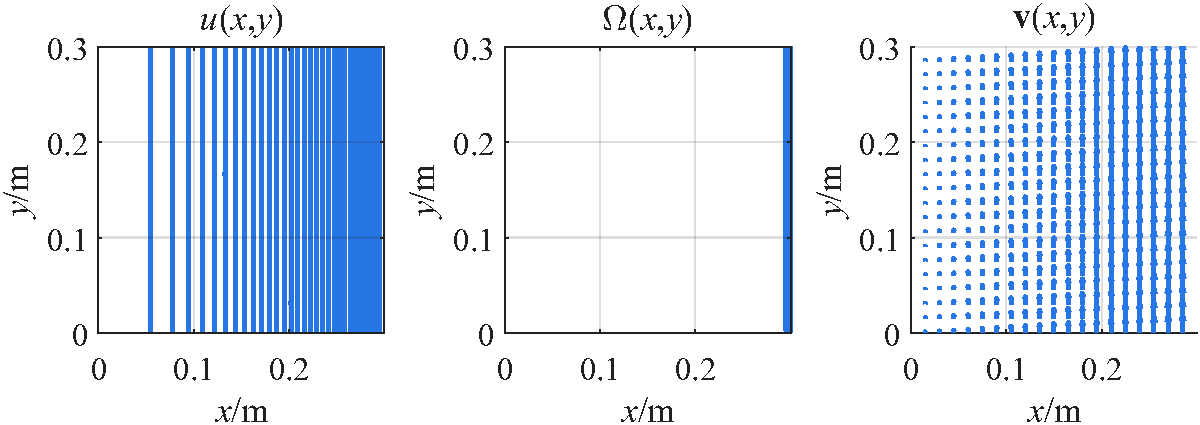
\includegraphics[width=0.8\textwidth]{HaftbWandLinearFelder}
  \caption[Haftbedingung an einer Wand mit linearem Geschwindigkeitsprofil]
  {Haftbedingung an einer Wand. Links haftet das Fluid an einer Wand, rechts
    bewegt es sich mit der Geschwindigkeit $v_0$. Es wird kein Druckgradient
    in $z$-Richtung angenommen. Gezeigt sind Linien f�r konstantes $u(y,z)$
    und konstantes $\Omega(y,z)$ sowie das Geschwindigkeitsfeld.}
  \label{abb:aero_RandDruck0Felder}
\end{figure}
%
Betrachtet man das Geschwindigkeitsprofil (entlang des mittleren Wertes von
$z$) sieht man eindeutig das lineare Geschwindigkeitsprofil in
\figref{aero_RandDruck0Profil}.
%
\begin{figure}[tbp]
  \centering
  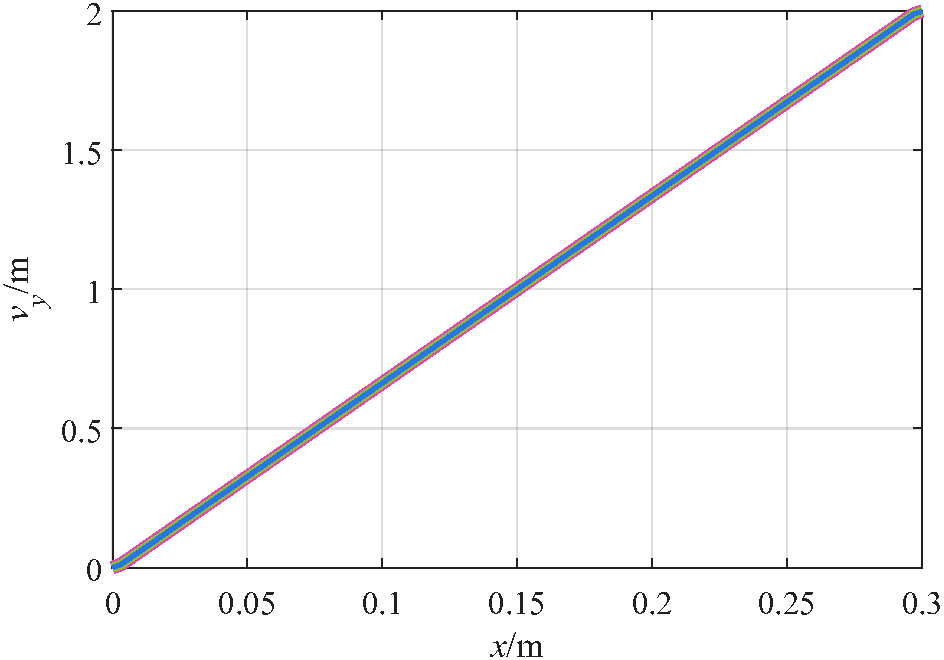
\includegraphics[width=0.5\textwidth]{HaftbWandLinearProfil}
  \caption[Lineares Geschwindigkeitsprofil an einer Wand]
  {Lineares Geschwindigkeitsprofil an einer Wand. Es liegt kein Druckgradient
    vor und $v(y)$ ist f�r den mittleren Wert von $z$ aus
    \figref{aero_RandDruck0Felder} dargestellt.}
  \label{abb:aero_RandDruck0Profil}
\end{figure}
%
F�r den Druckgradienten aus Fall \ref{item:aero_RandDruck1},
\begin{equation*}
  \frac{1}{2\eta} \frac{\partial p(z)}{\partial z} = \frac{v_0}{b^2} \; ,
\end{equation*}
sind $u(y,z)$, $\Omega(y,z)$ und das Geschwindigkeitsfeld in
\figref{aero_RandDruck1Felder} dargestellt.
%
\begin{figure}[tbp]
  \centering
  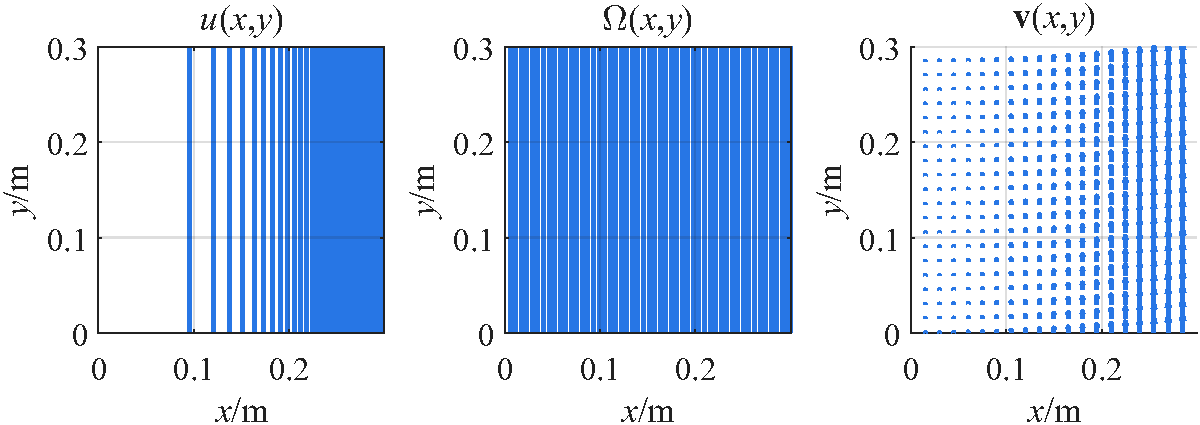
\includegraphics[width=0.8\textwidth]{HaftbWandScheitelLFelder}
  \caption[Haftbedingung an einer Wand mit parabelf�rmigen
  Geschwindigkeitsprofil und Scheitel an der Wand]
  {Haftbedingung an einer Wand. Links haftet das Fluid an einer Wand, rechts
    bewegt es sich mit der Geschwindigkeit $v_0$. Es liegt eine Druckgradient
    von $1/(2\eta)\, \partial p(z)/\partial z = v_0/b^2$ vor. Gezeigt sind
    Linien f�r konstantes $u(y,z)$ und konstantes $\Omega(y,z)$ sowie das
    Geschwindigkeitsfeld.}
  \label{abb:aero_RandDruck1Felder}
\end{figure}
%
In der Darstellung des Geschwindigkeitsprofils in
\figref{aero_RandDruck1Profil} sieht man eindeutig den Scheitel am linken
Rand.
%
\begin{figure}[tbp]
  \centering
  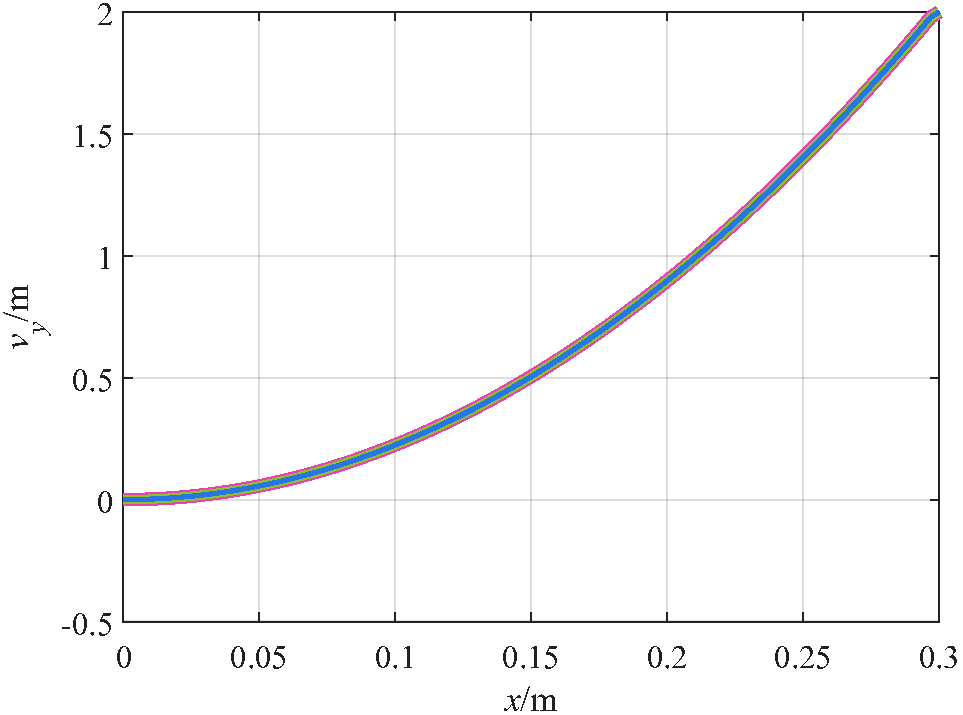
\includegraphics[width=0.5\textwidth]{HaftbWandScheitelLProfil}
  \caption[Parabelf�rmiges Geschwindigkeitsprofil mit Scheitel an der Wand]
  {Parabelf�rmiges Geschwindigkeitsprofil mit Scheitel an der Wand. Es liegt
    ein Druckgradient von $1/(2\eta)\, \partial p(z)/\partial z =
    v_0/b^2$ vor und $v(y)$ ist f�r den mittleren Wert von $z$ aus
    \figref{aero_RandDruck1Felder} dargestellt.}
  \label{abb:aero_RandDruck1Profil}
\end{figure}
%
Vollkommen analog findet man f�r den Druckgradienten aus Fall
\ref{item:aero_RandDruck2},
\begin{equation*}
  \frac{1}{2\eta} \frac{\partial p(z)}{\partial z} = -\frac{v_0}{b^2}  \; ,
\end{equation*}
die Werte $u(y,z)$, $\Omega(y,z)$ und das Geschwindigkeitsfeld aus
\figref{aero_RandDruck2Felder}.
%
\begin{figure}[tbp]
  \centering
  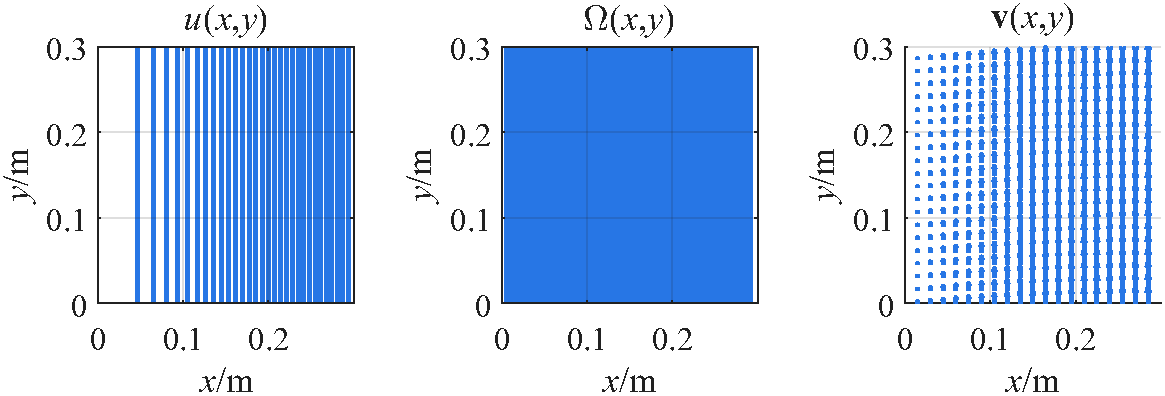
\includegraphics[width=0.8\textwidth]{HaftbWandScheitelRFelder}
  \caption[Haftbedingung an einer Wand mit parabelf�rmigen
  Geschwindigkeitsprofil und Scheitel an der Wand]
  {Haftbedingung an einer Wand. Links haftet das Fluid an einer Wand, rechts
    bewegt es sich mit der Geschwindigkeit $v_0$. Es liegt eine Druckgradient
    von $1/(2\eta)\, \partial p(z)/\partial z = -v_0/b^2$ vor. Gezeigt sind
    Linien f�r konstantes $u(y,z)$ und konstantes $\Omega(y,z)$ sowie das
    Geschwindigkeitsfeld.}
  \label{abb:aero_RandDruck2Felder}
\end{figure}
%
In der Darstellung des Geschwindigkeitsprofils in
\figref{aero_RandDruck1Profil} sieht man eindeutig, dass hier der Scheitel
am rechten Rand liegt, also dort, wo die Geschwindigkeit maximal ist.
%
\begin{figure}[tbp]
  \centering
  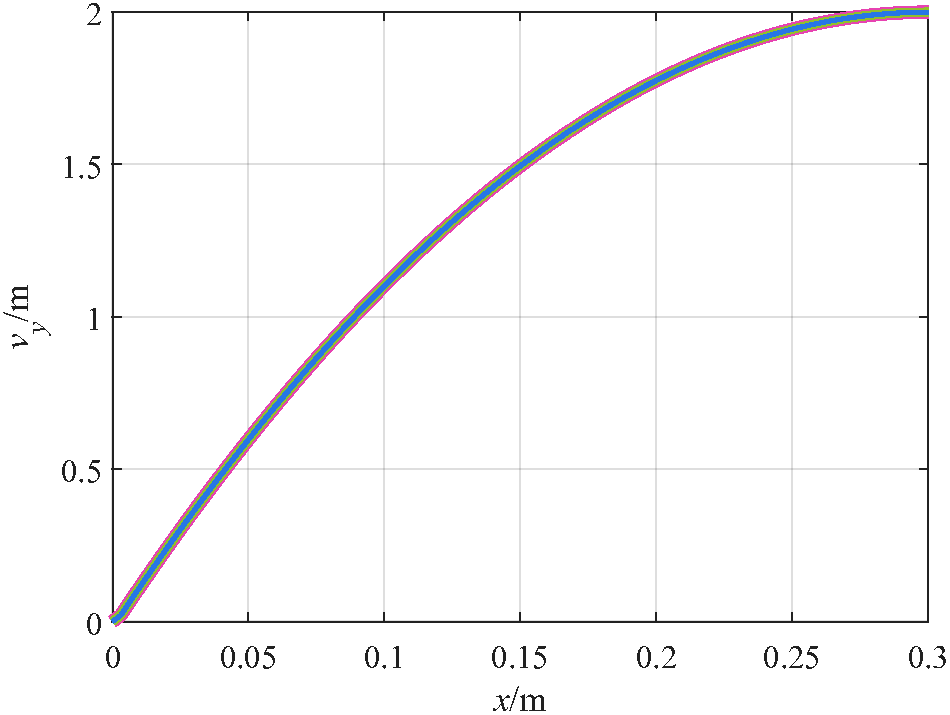
\includegraphics[width=0.5\textwidth]{HaftbWandScheitelRProfil}
  \caption[Parabelf�rmiges Geschwindigkeitsprofil mit Scheitel bei der
  maximalen Geschwindigkeit]
  {Parabelf�rmiges Geschwindigkeitsprofil mit Scheitel bei der maximalen
    Geschwindigkeit. Es liegt ein Druckgradient von $1/(2\eta)\, \partial
    p(z)/\partial z = -v_0/b^2$ vor und $v(y)$ ist f�r den mittleren Wert von
    $z$ aus \figref{aero_RandDruck2Felder} dargestellt.}
  \label{abb:aero_RandDruck2Profil}
\end{figure}
%


\end{sol} 
\textcolor{blue} {$\rightarrow$ zur} \probref{aero_haftwand}.\\
\noindent\rule[1ex]{\textwidth}{0.5pt}  \newpage  



\newpage


\section{\mscre}\label{kap:aero_matlabskripts}

Die mathematisch-physikalische Behandlung von Problem



\clearpage
\setcounter{chapter}{4}
\setcounter{section}{3}
\setcounter{subsection}{0}
\setcounter{figure}{0}
\setcounter{equation}{0}
\setcounter{prob}{0}
\counterwithin{table}{section}
\setcounter{table}{0}
\section{L�sungsbeispiele \autoref{chap:spo} -- Physik des Sports}\label{kap:spo_lsguebungen}

\begin{sol}{prob:spo_energyconsumption}\label{lsg:spo_energyconsumption} %�bung1
\textbf{Absch�tzung Energieverbrauch} \\ 

Text

\end{sol} 
\textcolor{blue} {$\rightarrow$ zur} \probref{spo_energyconsumption}.\\
\noindent\rule[1ex]{\textwidth}{0.5pt}  \newpage  


 
%


\section{\mscre}\label{kap:spo_matlabskripts}

Die mathematisch-physikalische Behandlung von Problem



%\newpage
%\thispagestyle{empty}
%\quad 
%\newpage
%\newpage
\end{PartL}

\renewcommand{\thechapter}{A\,\arabic{chapter}}

\begin{PartA}{Appendix}

\setcounter{chapter}{2}
\setcounter{section}{2}
\setcounter{subsection}{0}
\setcounter{equation}{0}
\counterwithin{table}{section}
\setcounter{table}{0}
\newpage
\thispagestyle{empty}
\quad 
\newpage
\newpage
\section{Formelsammlung zur Aerodynamik}\label{kap:aero_formelsammlung}
Im Folgenden geben wir zum Arbeitsbuch einige h�ufig benutzte Formeln und Beziehungen der Aerodynamik.




\newpage
\section{Formelsammlung zur Sportphysik}\label{kap:spo_formelsammlung}
Im Folgenden geben wir zum Arbeitsbuch einige h�ufig benutzte Formeln und Beziehungen der Sportphysik.


\newpage
\addcontentsline{toc}{chapter}{Quellenangaben}

\begingroup
\let\cleardoublepage\relax
\bibliography{referenzen}
\phantomsection
\addcontentsline{toc}{section}{Stichwortverzeichnis}
\printindex
\phantomsection
\addcontentsline{toc}{section}{Personenverzeichnis}
\printindex[personen]


\cleardoublepage
\phantomsection
\addcontentsline{toc}{chapter}{MATLAB-Skriptverzeichnis}
\thispagestyle{fancy}
\fancyhead[LO]{\nouppercase{\normalsize MATLAB-Skriptverzeichnis}}
\fancyhead[RE]{\nouppercase{\normalsize MATLAB-Skriptverzeichnis}}

\printindex[mfiles]


\endgroup
\newpage
\thispagestyle{empty}
\quad 
\newpage

\end{PartA}

%%%%%%%%%%%%%%%%%%%%%%%%%%%%%%%%%%%%%%%%%%%%%%%%%%%%%%%%%%%\cdot
%\input{footer.tex}
   

\input{footer} 


%%%%%%%%%%%%%%%%%%%%%%%%%%%%%%%%%%%%%%%%%%%%%%%%%%%%%%%%%%%%%%%%%%%%%%%%%%%%%%






